%% Styling TODOs:
% -> Try enabling \frenchspacing (don't double space sentences)
% -> Set a link color: \definecolor{LinkColor}{HTML}{80171F}
% -> Test drop caps and header from
%    https://github.com/sarabander/sicp-pdf/blob/master/src/preamble.tex

\documentclass[b5paper]{report}
\usepackage[lmargin=25mm,rmargin=25mm,tmargin=27mm,bmargin=30mm]{geometry}
\usepackage{microtype}
\usepackage{booktabs}
\usepackage{color}
\usepackage{xcolor}
\usepackage{tikz}
\usepackage{pgfplots}
\usepackage{graphicx}
\usepackage{wrapfig}
\usepackage{svg}
\usepackage{float}
\usepackage{url}
\usepackage{parskip}
\usepackage[hidelinks]{hyperref}
\usepackage[utf8]{inputenc}

%% Syntax highlighting:
\usepackage[chapter]{minted}

%% Chapter header:
\usepackage[Lenny]{fncychap}

%% Font:
% \usepackage{lmodern}
\usepackage[libertine]{newtxmath}
\usepackage{libertineRoman}
\usepackage{biolinum}
\usepackage{titlesec}
\titleformat*{\subsubsection}{\large\bfseries}

\graphicspath{{images/}}
\svgpath{{images/}}
\usetikzlibrary{positioning}
\usetikzlibrary{shapes,decorations,shadows}

% BibLaTeX for bibliography
\usepackage[
  backend=bibtex,
  style=numeric-comp,
  minalphanames=3,
  isbn=false,
  sortcites=true,
  sorting=anyt,
  abbreviate=false,
  url=false,
  doi=false,
  maxnames=6,
  minbibnames=3,
  maxbibnames=7]{biblatex}
\setlength\bibitemsep{5pt}
\addbibresource{sources.bib}

\definecolor{LinkColor}{HTML}{1C4883}
% Potential colors:
% SICP red: #80171F
\hypersetup{
  pdfauthor={Lars Martin Bævre Ek},
  pdftitle={Durability in a data-flow based storage system},
  colorlinks=true,
  linkcolor=LinkColor,
  urlcolor=LinkColor,
  citecolor=LinkColor,
}

\begin{document}

\begin{titlepage}
  \centering
	
\includegraphics[width=0.55\textwidth]{ntnu}\par\vspace{1cm}
	{\scshape\Large TDT4900 Master's Thesis \par}
	\vspace{1.5cm}
	{\huge\bfseries Durability in a data-flow based storage system\par}
	\vspace{2cm}
	{\Large\itshape Lars Martin Bævre Ek \\ \texttt{larek@stud.ntnu.no} \par}
	\vfill
	supervised by\par
  Professor Kjetil \textsc{Nørvåg}

	{\large \today\par}
\end{titlepage}

\newcommand{\note}[1]{{\color{olive}\sffamily #1}}
\newcommand{\todo}[1]{{\color{purple}\sffamily[TODO: #1]}}
\newcommand{\eg}{\textit{e.g.},\xspace}
\newcommand{\ie}{\textit{i.e.},\xspace}
\newcommand{\vs}{\textit{vs.}\xspace}
\newcommand{\viz}{\textit{viz.},\xspace}

% Handy superscript macros
\newcommand{\stss}{\textsuperscript{st}}
\newcommand{\ndss}{\textsuperscript{nd}}
\newcommand{\rdss}{\textsuperscript{rd}}
\newcommand{\thss}{\textsuperscript{th}}

% Enumeration commands
\newcommand{\one}{({\em i}\/)}
\newcommand{\two}{({\em ii}\/)}
\newcommand{\three}{({\em iii}\/)}
\newcommand{\four}{({\em iv}\/)}
\newcommand{\five}{({\em v}\/)}

\newcommand\code[1]{\texttt{#1}}


\tableofcontents
\pagebreak

\begin{abstract}
  \color{purple}
TODO:
\begin{itemize}
  \item Add more explanatory figures
  \item Use minipage for horizontal tables: https://tex.stackexchange.com/questions/101824/align-the-top-of-two-tables-horizontally-side-by-side-with-minipage

  \item Abstract

  \item Background Recovery
  \item Background Rust

  \item Background/Related Work: MyRocks
  \item Background/Related Work: CockroachDB
  \item Background/Related Work: Indexing scheme research
\end{itemize}

% \color{purple}
% Potential questions:
% \begin{itemize}
%   \item How often should references to previous sections be included? E.g., if a
%     phrase described in the Background section is used later on, should that
%     immediately warrant a reference to section x.x.x?
% \end{itemize}

\end{abstract}

\ChNameVar{\fontsize{14}{16}\usefont{OT1}{cmr}{m}{n}\selectfont}
\ChNumVar{\fontsize{60}{62}\usefont{OT1}{qpl}{m}{n}\selectfont}
\ChTitleVar{\Huge\bfseries\rm}, \ChRuleWidth{1pt}

\chapter{Introduction}

Building sophisticated web applications while scaling to potentially millions of
users forces developers to compromise between performance, user requirements,
and application complexity. Whereas traditional relational databases logically
are able to fulfill the increasingly complex storage demands of today's internet
businesses, they are far from able to do so at the scale and performance
required. To continue serving requests at increasing throughputs with low
latencies, developers introduce mitigation strategies ranging from complex cache
hierarchies~\cite{memcached} to denormalized schemas~\cite{denormalization}.

These methods are usually used to drastically improve read performance, while
penalizing write throughput and increasing application complexity.
Soup~\cite{xylem} sets out to solve this dilemma once and for all, with a
structured storage system capable of horizontally scaling to millions of reads
per second, without the need for complex cache deployments or manual maintenance
of materialized views.

Soup achieves this through use of an incrementally maintained data-flow graph.
New updates propagate through the graph at write-time, with pre-computed results
stored at selected \textit{materialized} nodes throughout the graph. This
moves the bulk of the workload from reads to writes, by allowing read operations
to directly access computed state from materialized nodes further down the
graph.

Soup ensures durability by persisting all updates to a write-ahead log before
they are injected into the data-flow graph. While appending entries to a file is
good for performance, recovering from an ever-growing log after a failure is far
from feasible. This thesis improves Soup's durability situation with two main
contributions: it moves Soup's otherwise in-memory table structures to durable
storage, and implements snapshotting of Soup's materialized views. Both
contributions were implemented in the open-source Soup prototype written in the
Rust programming language, and a list of the changes is available in appendix A.

\newpage

\section{From main-memory to durable storage}

After updates are persisted to Soup's write-ahead log, they are injected into
the first nodes in the data-flow graph: the base tables. Unlike the partially
materialized nodes further down the data-flow graph, the base tables can never
be evicted from, and must together always contain a full representation of a
Soup application's state. On the other hand, the base tables should only be
responsible for serving a small part of Soup's read queries. The rest should be
handled by materialized nodes towards the bottom of the graph, using state that
was pre-computed when the updates propagated through the data-flow graph.

This makes volatile main-memory a poor destination for Soup's base table data.
Applications where data is continuously inserted would cause Soup's memory
footprint to grow continuously over time, until eventually reaching its host
system's memory limit. Moving the base tables to durable storage avoids this
problem, while reducing Soup's overall memory usage.

Storing base tables on durable storage also improves Soup's recovery situation,
by avoiding the need to replay the entire write-ahead log after failures. With
all updates safely persisted to and readily available from durable storage,
recovery is instead a matter of replaying data from the base tables when needed.

\section{Snapshotting materialized views}

With durable base tables, Soup recovers significantly faster than by having to
replay the entire write-ahead log. This is not without downside however: whereas
log-based recovery brings all nodes in the data-flow graph back to a
pre-failure state, durable base tables leave partial nodes empty, resulting in a
latency penalty for initial read-queries. Instead, we would like to periodically
write \textit{snapshots} of the materialized state at each node to durable
storage, ensuring a speedy recovery process for both base tables and
materialized views alike.

To snapshot nodes individually while maintaining consistency, it is crucial that
all nodes snapshot the same window of updates. For a given update at any given
time, said update must either be contained in every snapshot across the graph,
or neither of them. While updates are processed synchronously within a single
domain in Soup (a partition of nodes), data flows asynchronously between
domains, where the boundaries can be both within a local machine and across a
network. At the same time, taking a snapshot should not incur a significant
pause in processing, which would result in lower throughput all around.

By approaching the problem from the viewpoint of snapshotting in a distributed
system, this thesis implements a snapshotting method capable of creating a
logically consistent snapshot across the data-flow graph, with a focus on
maintaining as much of Soup's performance guarantees as possible.

\section{Outline}

The rest of this thesis is structured as follows:

\begin{itemize}
  \item \textbf{Chapter~\ref{chap:background}} introduces core theory behind fundamental
  concepts used in the rest of this thesis.
  \item \textbf{Chapter~\ref{chap:related-work}} reviews ideas from research and
  industry relevant to the thesis' main contributions.
  \item \textbf{Chapter~\ref{chap:benchmarks}} describes new and existing
  benchmarks used throughout the thesis.
  \item \textbf{Chapter~\ref{chap:persistent-bases}} outlines the requirements
  for a persistent base table implementation, followed by two implementation
  iterations.
  \item \textbf{Chapter~\ref{chap:recovery}} gradually builds up a snapshotting
  implementation.
  \item \textbf{Chapter~\ref{chap:evaluation}} evaluates the resulting
  implementations from the two previous chapters, using the benchmarks
  introduced in chapter~\ref{chap:benchmarks}.
  \item \textbf{Chapter~\ref{chap:conclusion}} presents possible next steps
  towards a production-ready Soup, while concluding on the results presented
  earlier in the thesis.
\end{itemize}

\chapter{Background}\label{chap:background}

This chapter describes various concepts relevant to the rest of this thesis,
starting with an introduction to the system this thesis makes its contributions
to---Soup. Afterwards the Rust programming language is outlined, together with a
look at the \code{bincode} serialization library, which is used for both
snapshotting and persistent base tables. Following that, a few profiling
concepts are described, used to reason about performance issues throughout the
thesis. Finally, the two storage engines embedded in separate implementation
iterations of persistent base tables are studied.

% TODO: this sucks

\newpage

\section{Soup}

Soup~\cite{xylem} is an on-going research project at the Parallel and Distributed Operating
Systems\furl{https://pdos.csail.mit.edu/} group at MIT CSAIL.\@ The current Soup
prototype is written in the Rust programming language and made available as
open-source code on GitHub\furl{https://github.com/mit-pdos/distributary/}.

This section introduces Soup's core concepts.

\subsection{Data-flow}
\todo{figure that compares a traditional query graph to soup's data-flow}

Applications using Soup define base table schemas and a set of queries ahead of
time. Whereas the former is common in traditional relational database management
systems, the latter is not, and is the primary source of Soup's read performance
improvements. A relational database computes the result of queries on-the-fly,
by building a query-graph, which it then executes. This requires potentially
costly computations to be performed multiple times for separate queries, while
throwing away intermediary results that could be re-used. Soup instead builds a
\textit{data-flow} graph from its pre-defined queries, propagating each update
through it at write-time. Computations can then be incrementally maintained on
each write, reducing the work needed by a read-operation to something more
similar to a simple key-value read in a caching system.

\begin{listing}[H]
  \begin{minted}[frame=lines]{sql}
CREATE TABLE Car (id int, brand varchar(255), PRIMARY KEY(id));
QUERY CountCars: SELECT COUNT(*) FROM Car WHERE brand = ?;
  \end{minted}

  \caption{An example base table with a corresponding
  query.}\label{lst:example-schema}
\end{listing}

Implemented naively, incrementally maintaining a data-flow graph for each query
would have disastrous storage consequences. Each query would need a separate
graph, duplicating data across a range of nodes. Instead, Soup builds a single
data-flow graph from all of its queries, recognizing common sub-expressions
where possible~\cite{common-expression}. That still leaves the issue of what
state to incrementally maintain. With queries consisting of a potentially large
amount of nodes, materializing data at each step would lead to significant
overlap between nodes. Instead, Soup only materializes and incrementally
maintains state at nodes it considers \textit{stateful}, with other nodes
referring upwards in the graph to its closest materialized ancestor node.

The state at these materialized nodes is also kept \textit{partial} whenever
possible. Instead of storing the results for all queries---like a materialized
view does---Soup only retains state for records in the application's working
set, evicting rarely used data. Queries for missing keys result in ancestor
queries---\textit{replays}---to nodes further up the graph. Similar to cache
misses in other systems these eventually propagate all the way up to the base
nodes, where a full copy of the state is always maintained.

\subsubsection{Migrations}

Schema migrations are inevitable in long-running applications: business
requirements change, projects are refactored, and new features are added.
Performing migrations in traditional database systems, without downtime, is on
the other hand far from trivial~\cite{stripe, gh-ost}. While Soup requires both
the schema and all queries to be defined ahead of time, it handles changes in
both seamlessly.

Added queries extend the existing data-flow with additional nodes, while
re-using as much as possible of the existing graph. New partially materialized
nodes can start serving requests right away, by fetching data from ancestor
nodes if necessary. This is not the case with fully materialized nodes, which
require a full representation of their state at all times. To bring these nodes
online, Soup incurs a full replay of the state needed, potentially delaying new
requests until all replays have completed. Review of the migrations performed
during the lifetime of the HotCRP conference review
program~\cite{hotcrp}---which uses MySQL---showed that these delays were rare,
with Soup being able to transition 95\% of schema changes without downtime.

\todo{figure of a changing data-flow graph}

Changes to the base table schema happen in-place, and Soup's base nodes retain a
full history of columns for each table. This ensures that both existing and new
requests can be served alongside each other, allowing the data-flow graph to
transition without downtime.

\subsubsection{Domains}

Soup's data-flow graph is partitioned into \textit{domains}, each containing a
series of nodes. Updates are processed at separate domains asynchronously, in
different computational units---threads, or other machines altogether for
distributed Soup. Within a single domain, packets are processed synchronously,
one at a time, removing the need for locking within domains. Packet processing
at domains include both regular updates and other types of packets, such as
replay requests.

\todo{figure that shows different domains}

Domains are separated by egress and ingress nodes, responsible for maintaining
communication across domain boundaries using a buffered channel. When Soup is
run in a distributed fashion, communication between separate domains happen
over TCP sockets, between the egress and ingress nodes.

\subsubsection{Sharding}

Distributing domains across computational units lets Soup divide its processing
load between a cluster of machines. This is only an improvement if the load is
uniformly spread across all domains. When that is not the case, and a majority
of the data is skewed towards a single domain, Soup is left to processing most
of the requests in a single computational unit. This is where sharding comes in.
By splitting the atom that is a single domain into multiple shards, both the
computational load and the data stored at that domain can be spread between
multiple computational units.

\todo{show a figure with a sharder?}

Balancing the data across a cluster is essential in scaling Soup to larger
datasets. Without sharding, Soup's capabilities would be capped at the memory
size of the largest machine in the cluster. Soup shards data by
hash-partitioning keys statically. This is unfortunate for workloads skewed
towards a small key subset, where only a few domains might end up serving most
of the requests received. Dynamic sharding would evenly re-balance the workload
across the shards, and is a future implementation goal for Soup.

When necessary, a \textit{sharder} node is inserted between domains, translating
between sharding schemes in separate domains. This allows nodes further down in
the graph to remain partial, at the cost of having to replay state across
domains.


\subsubsection{Eviction}\label{sec:eviction}

To ensure that partial state does in fact remain partial over time, Soup evicts
data when necessary. Currently this happens when Soup's memory-limit goes beyond
an application-defined limit. This triggers an eviction notice sent to the
largest domain---measured in state-size---which then takes care of propagating
this eviction notice downstream in the graph to any nodes that might depend on
the evicted state.

\todo{might not be necessary, but could have an eviction figure here}

The keys to evict at a specific node are picked randomly. In the future, this
could be improved through more sophisticated eviction strategies, such as only
evicting the least-recently used records.

\subsection{Operators}

Soup's data-flow graph consists of relational operators, where each operator
emits either the \code{Positive} or the \code{Negative} records required for
downstream nodes to maintain their state accordingly.

\subsubsection{Base nodes}

Every packet that reaches Soup is first injected into an appropriate base node,
similar to a table in a relational database. This is where external API requests
are translated into a language the rest of the data-flow graph understands.
While clients might issue \eg deletion requests by \textit{key}, the base nodes
translate the request into a \code{Negative} record for the entire row, which
the rest of the data-flow graph can use to invalidate removed state. Update
requests are likewise first translated into a \code{Negative} record, followed
by a \code{Positive} record containing the new row.

Whereas other stateful nodes can keep their state \textit{partial}, choosing
which records to maintain and which to discard, base nodes always remain fully
materialized at all times.

\subsubsection{Stateless operators}

Stateless operators process updates with no regard for prior events, without
maintaining any state at all. The operators that fall within this category are
\textit{pure functions}, such as the \textit{projection} and \textit{filter}
operators. The former pick out one or more fields from each incoming row, while
the latter determines if a row should be forwarded through the data-flow graph
or not.

While Soup is free to insert operators into its data-flow graph as it sees fit,
both projections and filters can often be mapped directly to a part of an SQL
query. \code{SELECT name \dots} would result in the projection shown in
figure~\ref{fig:project}, while a \code{WHERE}-clause on the form of \code{WHERE
age < 10} would produce a filter operator emitting only records where \code{age
< 10} is true.

\begin{figure}[H]
  \centering
  \includesvg[width=0.3\textwidth]{project}
  \caption{A projection operator responsible for picking out the \code{name}
  column of incoming records.}\label{fig:project}
\end{figure}

\subsubsection{Stateful operators}

Whereas stateless operators resemble their counter-parts in relational
databases~\cite{codd}, Soup's stateful operators compute results incrementally
by maintaining internal state between updates. This saves Soup from re-doing
potentially expensive computations, by instead mutating the previous result when
a new record arrives. The \textit{count} operator---produced by a SQL
\code{COUNT}-clause---is an example of a stateful operator, where
\code{Positive} and \code{Negative} records incur an addition or subtraction of
the current count, respectively. Another example is the \textit{top-k} operator,
produced by \eg an \code{ORDER BY}-clause coupled with a \code{LIMIT} to
determine the $ k $ most significant or insignificant elements.

\begin{figure}[H]
  \centering
  \includesvg[width=0.3\textwidth]{max}
  \caption{\
    The \textit{max} operator emits both a negative and a positive record when
    its state changes: the former to signal that its previous state should be
    invalidated, the latter to inform downstream nodes of the new result.
  }
\end{figure}

\subsubsection{Joins}

Finally, Soup supports joining together multiple paths of the data-flow graph.
This is made possible using \textit{ancestor queries}. Whenever a record arrives
at a join operator, it queries its other ancestors for the records required to
produce a single, unified update. To make sure that this is completed in an
efficient manner, join operators force their ancestors to retain indices on the
fields that they need to be queried for.

\begin{figure}[H]
  \centering
  \includesvg[width=0.7\textwidth]{join}
  \caption{\
    An ancestor query is performed to the right side of the join to produce a
    unified record for the update received from the left.
  }
\end{figure}

\subsection{Eventual consistency}

Databases are often considered the source of truth for applications, and
anomalies here could have disastrous consequences. Whereas fatal failures are
easy to recognize, unexpected behavior at the data layer could be the exact
opposite. This is a convincing argument for strong consistency, where the result
of all operations can be reasoned about from the ordering and type of operation
performed.

Regardless, companies scaling web applications to large amounts of users often
opt for systems with lesser consistency guarantees~\cite{dynamo, pnuts, werner}.
While the performance of strongly consistent systems have taken a turn for the
better with the introduction of horizontally scalable systems with clearly defined
consistency guarantees~\cite{spanner, cockroach}, the race is still far from
even when compared to systems with lesser consistency guarantees. At the same
time, the question of whether strong consistency is actually a requirement for
most applications remain. Analysis of live requests at
Facebook~\cite{existential} showed the opposite: only 0.0004\% of reads would
have returned different results in a strongly consistent system with total
ordering. These cases could then be handled explicitly, avoiding the need to
penalize the performance of an entire system for a fraction of the requests.

Soup targets applications where eventual consistency is sufficient, and would
not be able to provide the performance it does without it. Eventual consistency
avoids the need for explicit synchronization on every update, while allowing
Soup to scale in a distributed fashion without a total ordering of writes.
Clients receive write acknowledgments for writes when updates have been safely
persisted to durable storage, after which they are propagated through Soup's data-flow
graph asynchronously.

Reads access double-buffered hash tables directly~\cite{evmap}, without the need
for locks. Writes update one of the buffers, and expose updated content to the
readers with an atomic swap.

% TODO: maybe write a little more about the readers here

\subsection{Architecture}

\todo{figure}

\subsubsection{Controller}

At the heart of Soup lies a replicated controller, with a leader elected
using ZooKeeper~\cite{zookeeper}. The controller is the first point of contact
for Soup's external APIs, and is responsible for managing meta state, such as
schemas and queries.

\subsubsection{Souplets}

Processing of updates happen within the Souplets---Soup's worker nodes. Each
Souplet includes a pool of threads which together go through the incoming
packets for its domains. While maximum one thread can process updates for a
domain at once, multiple domains can process updates in parallel. Earlier
versions of Soup ran domains in separate threads altogether, resulting in a
core-constrained system when the number of domains went far beyond the host's
CPU core count.

Communication between the Souplets and the controller happens over TCP, at the
coordination layer.

\subsubsection{Readers}

Soup's reader nodes make use of double-buffered hash tables to make it possible
to read and write to a single data structure at the same time. To prevent high
throughput write processing from slowing down reads, read requests are processed
by separate threads---readers.

\subsection{Interacting with Soup}

Applications using Soup define a base table schema and a set of corresponding
queries. The query syntax resembles that of prepared statements in relational
databases, where placeholders are replaced with values when the query is used in
a read operation. Both the schema and the queries can be modified and extended
later on, through Soup's external API.\@

\begin{listing}[H]
  \begin{minted}[frame=lines]{sql}
/* Base table schemas: */
CREATE TABLE Article (aid int, title varchar(255),
                     url text, PRIMARY KEY(aid));
CREATE TABLE Vote (aid int, uid int);

/* Intermediate view (not exposed through the client): */
VoteCount: SELECT Vote.aid, COUNT(uid) AS votes
            FROM Vote GROUP BY Vote.aid;

/* Read query: */
QUERY ArticleWithVoteCount:
            SELECT Article.aid, title, url, VoteCount.votes AS votes
            FROM Article, VoteCount
            WHERE Article.aid = VoteCount.aid AND Article.aid = ?;
  \end{minted}
  \caption{Soup schema with two base tables and an external query.}\label{lst:soup-schema}
\end{listing}

Writing to and reading from Soup is done through mutators and getters. Both are
built by going through the controller, after which writes can go directly to the
domain and reads can access readers directly.

\begin{listing}[H]
  \begin{minted}[frame=lines]{rust}
// Build mutators and getter.
let mut article = blender.get_mutator("Article").unwrap();
let mut vote = blender.get_mutator("Vote").unwrap();
let mut awvc = blender.get_getter("ArticleWithVoteCount").unwrap();

// Insert a new article:
let aid = 1;
let title = "new article";
let url = "https://ntnu.edu";
article
  .put(vec![aid.into(), title.into(), url.into()])
  .unwrap();

// Vote for the article:
let uid = 123;
vote
  .put(vec![aid.into(), uid.into()])
  .unwrap();

// Read the vote count:
println!("{}", awvc.lookup(&[aid.into()], true));
  \end{minted}

  \caption{Soup example usage, where an article and a vote is inserted,
  followed by a read of the vote count.}\label{lst:soup-api}
\end{listing}

\subsection{MySQL Protocol Translation}\label{sec:mysql-shim}

Soup supports a decent subset of SQL in its query definitions. Regardless, using
Soup in an application requires significant changes: all queries have to be
defined ahead of time, and interactions with Soup have to go through Soup's
external API.\@ Soup's MySQL shim~\cite{soup-mysql} makes this easier by letting
applications communicate with Soup using the MySQL binary protocol.

The MySQL shim acts as a separate service, which clients interact with over
TCP.\@ Received queries extend the Soup data-flow graph if needed, before they
are forwarded to an appropriate Soup worker for execution.

% TODO: maybe write a little more

\section{SQLite}\label{sec:sqlite}
SQLite~\cite{sqlite} is by far the most widely deployed database ever written.
Used in everything from smart phones to cars, with an estimated user count in
the magnitude of multiple billion users, SQLite is everywhere\footnote{Who
uses SQLite? \url{https://www.sqlite.org/mostdeployed.html}}. SQlite is an
embedded database, and requires no extra processes, or even threads, to run.

In a world of unreliable software, SQLite is stable as a rock. It has 100\%
branch test coverage, with a test suite containing millions of different test
cases. SQLite is, and always has been, available in the public domain. As the
name implies, SQLite provides an SQL interface to developers, with decent support
for everything from indices to views. The library itself is written in about 130
thousand lines of C code.

While the main usage of SQLite is as a persistent application store (\eg in
browsers and mobile applications), SQLite is also popularly used as an engine in
other databases. One such example is the recently open-sourced
FoundationDB~\cite{foundation}, which provides a distributed database with full
ACID transactions, where each shard makes use of SQLite at its core.

\subsection{B-trees}\label{sec:btree}
Similar to a significant amount of other relational databases, SQLite makes use
of B-trees~\cite{btree} for its on-disk index structures. This is with good
reason: B-trees are well suited for mediums that perform better with larger
blocks of data, such as traditional spinning hard drives. While it has never
been officially decided what the B in B-tree stands for, a B-tree is a
self-balancing binary tree data structure.

Unlike other tree structures, such as binary search trees, each node in a B-tree
holds multiple values. By keeping the amount of values in a node---the node
size---close to the size of a block on disk, most of a B-tree's operations can
be performed in $ O(\log_b n) $ disk reads, where $ b $ is the maximum number of
entries per block, and $ \log_b n $ the height of the tree. With traditional
storage mediums, where a single disk seek might take multiple milliseconds, this
is extremely important.

\todo{Include a figure of a B-tree and a B+tree perhaps?}

When the term B-tree is used in database systems today, it is usually used to
refer to an improved version of the traditional data structure, and known as a
B+-tree. Whereas the former stores values in all levels of the tree, the
specialized version only does so at the leaf level, with the internal nodes only
containing copies of the keys. Actual records can then be stored in a different
on-disk data structure, with pointers from the leaf nodes, and by introducing
sibling pointers at the leaf node level, range queries can be efficiently
executed by walking the bottom of the tree horizontally.

\subsection{Rollback journal}\label{sec:sqlite-locks}
SQLite implements support for atomic transactions through the use of a rollback
journal. A historic copy of values prior to changes are kept in a separate
file---the rollback journal---so that they can be copied back to the actual
database file in the event of a \code{ROLLBACK}. Similarly, this file can be
deleted after a \code{COMMIT} of the transaction.

With a rollback journal, SQLite requires a full exclusive lock to be held for
the duration of all mutations to prevent file corruption, blocking any potential
readers from accessing the database. This is the main reason SQLite is commonly
not used as the storage system for applications that require high-performance
concurrent access to their database (\eg web application backends with multiple
active users): only a single write operation could be performed at the time.
This is not the case with reads, which hold shared locks.

\subsection{Write-ahead log}\label{sec:sqlite-wal}
In version 3.7.0, SQLite introduced an alternative to the traditional rollback
journal: the write-ahead log~\cite{sqlite-wal}. Maintaining the same atomicity
and durability guarantees, the use of a WAL significantly improves write
performance by catering to more sequential disk access. Additionally, reading
can now co-exist with writing, as writers do no longer block read access.

While the original rollback journal format writes directly to the database file,
maintaining old values in the rollback journal, SQLite in WAL-mode does the
opposite. Updates are appended to the WAL, and copied over to the main database
file when a \textit{checkpoint} is taken. This is also the reason readers can
continue to access the database while writes are happening, as the database file
itself is not mutated, only the WAL.\@

This introduces a slight performance penalty for reads however, as there are now
potentially two sources of truth for all content: the main database file, and
the WAL until a checkpoint happens. The longer the WAL is, the more time has to
be spent searching through it by reads.

\subsection{Interacting with SQLite}
Most applications interact with SQLite through its C-API, compiling SQL
queries into prepared binary statements, which can then be executed efficiently
with different arguments, as shown in listing \ref{lst:sqlite}.

\begin{listing}[H]
  \begin{minted}[frame=lines]{c}
sqlite3 *db;
sqlite3_stmt *statement;
char *err_msg = 0;
sqlite3_open("test.db", &db);
sqlite3_exec(
  db,
  "CREATE TABLE data (id INTEGER PRIMARY KEY)",
  NULL,
  NULL,
  &err_msg
);

// Compile a prepared statement:
sqlite3_prepare_v2(
  db,
  "INSERT INTO data VALUES (?1)",
  -1,
  &statement,
  0
);

// Then insert a single row with the value 10:
int id = 10;
sqlite3_bind_int(statement, 1, id);
  \end{minted}

  \caption{Simple SQLite C-example showing how to write a single row (error
  handling ignored for brevity)}\label{lst:sqlite}
\end{listing}

In addition, most programming languages have at least one popular library for
accessing SQLite, abstracting away the need to directly call into the C-bindings
through more idiomatic APIs for each language. SQLite also provides a
command-line interface, which can be used to directly read from and modify a
database with SQL statements.

\subsection{SQLite from Rust}
Accessing SQLite from Rust can be done through the excellent \code{Rusqlite}
library~\cite{rusqlite}, which
provides a Rust API on top of SQLite's C-bindings.

\begin{listing}[H]
  \begin{minted}[frame=lines]{rust}
let conn = Connection::open("test.db").unwrap();
conn.execute(
  "CREATE TABLE data (id INTEGER PRIMARY KEY)",
  &[],
).unwrap();

// Compile a prepared statement:
let statement = conn.prepare("INSERT INTO data VALUES (?1)").unwrap();

// Then insert a single row with the value 10:
let id = 10;
statement.execute(&[&id]).unwrap();

  \end{minted}

  \caption{SQLite example using \code{rusqlite} showing how to write a single
  row.}\label{lst:sqlite-rust}
\end{listing}

\section{RocksDB}\label{sec:rocksdb}
RocksDB is an embedded key-value store optimized for modern flash storage.
RocksDB started out at Facebook, with the goal of making a version of Google's
LevelDB that performed well on modern hardware. Today, RocksDB is used at the
heart of a wide variety of databases, such as CockroachDB~\cite{cockroach},
MyRocks~\cite{myrocks} and TiDB~\cite{tidb}.

Traditional B-tree based database systems are often faced with poor write
performance as a result of random writes, which perform worse than sequential
writes on both magnetic and flash based storage mediums. RocksDB, on the other
hand, achieves impressive write performance through the use of immutable
log-structured merge trees~\cite{lsm} (LSM-trees), avoiding the need for random
writes to persistent storage altogether.

Writes are initially only written to a persistent write-ahead log (WAL) and
in-memory data structures referred to as memtables. Later, these memtables are
flushed to their equivalent data structures on disk, Static Sorted Tables (SST).
The latter is done by background threads, allowing regular processing to
continue without getting blocked by slow writes to persistent storage. Both of
these components originate in Patrick O'Neil's original paper on
LSM-trees~\cite{lsm}, where the in-memory data structure is referred to as $ C_0
$, and the on-disk structures $ C_{1..n} $.

% TODO:
% * Calling into RocksDB (C-API, rust-rocksdb)
% * Iterators
% * Prefix Iteration/Slice Transform

\subsection{MemTables}
All writes are initially synchronously written to an in-memory data structure---a
memtable---which is later flushed to disk at the point of filling up. Both the
size and the number of memtables can be configured at runtime.

RocksDB's default memtable implementation is a skiplist, with an $ O(\log n) $
bound on inserts, searches and deletes. This can be changed to a series of hash
based implementations, which offer better performance if all operations are done
within a pre-specified key prefix.

\subsection{Static sorted tables}
After a memtable reaches a certain size, RocksDB's background threads takes over
and flushes it to persistent storage. This will generate one or more SS-tables
on disk, where each file is sorted. SS-tables are immutable: a new SS-table is
always created, and existing ones are never updated. This ensures that writes
remain sequential.

\subsection{Write-ahead log}\label{sec:rocksdb-wal}
RocksDB achieves durability through the use of a write-ahead log (WAL). Without
it, data in memtables would be lost at the event of a crash. By default, every
\code{Put} operation results in a write to the RocksDB WAL, with the optional
possibility of waiting for the write to be fully synchronized to the WAL before
returning.

Each memtable corresponds to a WAL-file, which is marked as obsolete when the
memtable has been safely persisted to disk. Each WAL-file includes a sequence
number, and the files are iterated through in order during recovery. The WAL
itself is built up of a sequence of records, where each record includes a
computed cyclic redundancy check hash over the payload, to maintain
integrity~\cite{rocksdb-wal}.

Optionally, the WAL can be written to a different disk than the regular database
files. This is essential for production systems that want to maintain a high
write throughput: compactions and memtable flushes can then utilize the full
disk capacity without slowing down the throughput of WAL writes. Even more
drastically, the database files could be written to faster, volatile storage,
relying solely on never-archived WAL-files for (albeit much slower) recovery.

\begin{listing}[H]
  \begin{minted}[frame=lines]{rust}
let batch = WriteBatch::default()
batch.put("a", "1");
batch.put("b", "2");

let opts = WriteOptions::default();
opts.set_sync(true);
db.write(batch, &opts);
  \end{minted}

  \caption{Rust code for safely persisting a batch of writes to RocksDB and its
  write-ahead log.}\label{lst:write-batch}
\end{listing}

\code{Put} operations can also be batched into a \code{WriteBatch} (as shown in
listing~\ref{lst:write-batch}), to amortize the cost of synchronizing the WAL
over a larger amount of write operations. This is an atomic operation: either
all the writes in the write batch succeed, or none do.

\subsection{Basic operations}
Akin to other key-value databases, RocksDB offers a familiar API of
\code{Put(key, value)}, \code{Get(key)} and \code{Delete(key)}, operating
directly on bytestream values. Both insertions and deletions are purely
sequential: subsequent \code{Put} operations of the same key never backtrack and
overwrite existing keys, and deletions insert tombstone markers to avoid having
to randomly read and mutate previously written values.

Whereas both memtables and SS-tables are sorted, each tree structure has the
possibility of overlapping with another. This is a result of the immutability
property, and newly created SS-tables might contain key ranges already included
in existing structures. This means that read operations in RocksDB, and other
LSM-tree based storage systems, have to iterate through each tree
structure---starting with the memtables---in an attempt to find the key in
question. Reads within each sorted tree structure can be done in $ O(\log n) $
through a binary search. Going through a potentially large amount of SS-tables
on disk is costly however, and RocksDB employs a series of tricks to avoid doing
so.

\subsection{Compactions}\label{sec:compactions}

To maintain immutability, new SS-tables are always created without modifying
existing on-disk content. Two writes to the same key can thus co-exist in
different SS-tables, even if only the last written key is relevant to the
system. This is quite wasteful, and would lead to worse and worse read
performance over time. The original LSM-paper~\cite{lsm} solves this through
\textit{merging} existing LSM-trees into new ones at regular intervals. RocksDB
does so in background threads, where it is referred to as \textit{compaction}.

During compacting, multiple SS-tables are merge-sorted into a single new
structure. This process also removes duplicate keys, retaining only the last
value for future use. Tombstones are also filtered out, together with any values
they might have deleted.

\begin{figure}[H]
  \centering
  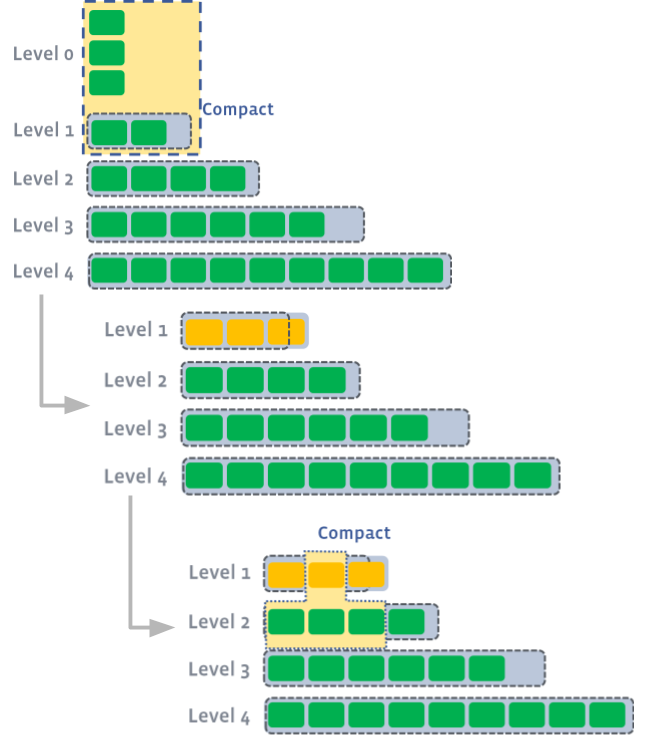
\includegraphics[width=0.5\textwidth]{level_compaction}
  \caption{SS-tables from initial levels are compacted into the next~\cite{rocksdb-compaction}.}
\end{figure}

In RocksDB, compactions are triggered when the previous \textit{level} reaches a
certain size. Referred to as \textit{leveled compaction}, this was one of the
original contributions of LevelDB\@. As described in~\cite{rocksdb-compaction},
this is usually initiated when the amount of SS-tables at the first level, level
0, goes beyond a certain amount. This in turn might cause the next level to go
beyond its size limit, resulting in a compaction to the next level again, and so
on. Unlike LevelDB, RocksDB also supports doing compactions in parallel, as long
as there are enough available background threads to do so.

\subsection{Bloom filters}\label{sec:bloom}

Iterating through every SS-table available to find a single key is inefficient.
Instead, we would like to ask the question ``can this key possibly exist here?''
for each of the SS-tables we go through, and only operate on the ones where the
answer is affirmative. With a regular hash based data structure this would be
quite costly in terms of space, as we would need to maintain such a structure
for every SS-table in our database. Instead, RocksDB, and many other systems
like it, rely on a probabilistic data structure known as a bloom
filter~\cite{bloom} to do so.

Instead of knowing with 100\% certainty whether a key exists in a set, a bloom
filter would let us know if that key \textit{might possibly} be in the set, or
if it is \textit{definitely} not. The third option, of \textit{possibly not}
being in the set, is impossible. The positive trade-off here is that it uses
significantly less space, allowing it to be used for every SS-table in the
system.

\subsection{Iteration}
One of the essential features of RocksDB compared to other key-value stores is
that its data is \textit{sorted}, and that it can be queried as such through
\textit{iterators}. This opens for a wide variety of possibilities that would
not have been feasible with a regular key-value store, such as range queries.
RocksDB supports iterating both forwards and backwards.

Similar to with reads, performing a fully ordered scan in an LSM-tree based
storage engine is far from optimal: every tree-structure, or SS-table in
RocksDB, needs to be considered, and as key ranges may overlap between different
files, sorted.

A lot of applications do not rely on completely random scans of keys however,
and only need support for ordered queries within a specific \textit{key prefix}.
Developers instruct RocksDB on how to retrieve a specific prefix from each key,
which RocksDB then internally uses to organize the data in such a manner that
iterating through keys within a \textit{specific prefix} is efficient: either by
storing bloom filters for each prefix, or by managing a hash based index
structure based on the prefix.

% TODO: might show an example to better explain prefix stuff here, or save it
% for implementation.

\subsection{Column Families}

RocksDB supports the equivalent of tables from a traditional database through
\textit{column
families}\furl{https://github.com/facebook/rocksdb/wiki/Column-Families}.
Separate column families share the same write-ahead log but have their own
MemTables and SS-tables. Maintaining the same WAL makes it possible to
atomically write across multiple column families, while keeping independent
LSM-tree components open for the possibility of configuring different column
families separately---an important difference from tables in SQL databases.

Column family support was not added until version 3.0 of RocksDB.\@ To maintain
backwards compatibility, the default API methods operate on the same column
family, ``default'', with separate methods taking in an additional column family
argument.

\subsection{Customizing the MemTable implementation}\label{sec:memtable-impl}

RocksDB provides multiple implementations of its in-memory
MemTables\furl{https://github.com/facebook/rocksdb/wiki/MemTable}, which can be
changed between through \textit{factories}. Different implementations have
different advantages and disadvantages, with the default being the all around
safest choice.

\subsubsection{Skip list}

The default implementation uses a \textit{skip list}, a data structure with
comparable performance guarantees to a binary search tree---$ O(\log n) $ for
searches, insertions and deletions---but with far better support for concurrent
operations. This makes the default skip list implementation the only MemTable
factory capable of concurrent insertions. Flushing a skip list MemTable to disk
is also considerably faster compared to the other factories, with a much lower
memory overhead.

\subsubsection{Hash skip list}

RocksDB provides two hash based MemTable factories, where keys are organized in
buckets based on their extracted \textit{prefix}. This implies that the hash
based implementations are only usable when a prefix extractor is defined, and
that they only support efficient iterations within a specific prefix. At the
same time, the hash based implementations are also considerably more efficient
when that is the case, providing $ O(\log k) $ performance, where $ k $ is the
number of keys within a specific prefix (which is often quite low).

\subsubsection{Hash linked list}

Similar to the skip list based hash table, RocksDB also provides a hash based
implementation where each bucket is maintained as a linked list instead of a
skip list. This is similar to a traditional hash table with chaining as its
collision resolution, and maintains close to constant time performance
guarantees as long as the elements in each bucket is kept low. This comes with
significantly lower memory overhead compared to the skip list based hash table,
but with naturally lower performance when the amount of keys per prefix starts
to grow. Because of this, the buckets in a \code{HashLinkList} are implicitly
converted to a skip list when its element count exceeds a certain threshold (256
by default).

\subsubsection{Vector}

Finally, RocksDB also provides a MemTable factory heavily tuned for random
insertions, with abysmal performance for everything else. This makes it only
useful for bulk loading data as fast as possible.

\subsection{Customizing the SS-table implementation}\label{sec:ss-table}

The default SS-table implementation is based on the original format from
LevelDB,
\code{BlockBasedTable}\furl{https://github.com/facebook/rocksdb/wiki/Rocksdb-BlockBasedTable-Format}.
As the name implies, data is stored in separate blocks, where each file's
initial block is a filter on the rest of the contents. The size of a single
block is usually fixed and can be configured by the application. Read operations
always read an entire block into memory, before searching for a specific record.
Previously read blocks are maintained in an in-memory cache---a block cache.

RocksDB also provides an improved format designed for low query latency on
modern storage media,
\code{PlainTable}\furl{https://github.com/facebook/rocksdb/wiki/PlainTable-Format}.
The format was initially developed for in-memory databases, but performs well on
other high performance mediums as well. Unlike \code{BlockBasedTable},
\code{PlainTable} addresses records by row, and uses a hash based in-memory
index for efficient reads. Similar to the hash based MemTable formats described
in section~\ref{sec:memtable-impl}, it uses \textit{prefix extraction} to place
keys into separate buckets. This also limits seek-based iteration to a single
prefix.

\subsection{RocksDB from Rust}\label{sec:rust-rocksdb}
While RocksDB is written in C++, it provides a separate API through its
C-bindings, which are used to call into it from a variety of different
languages\furl{https://github.com/facebook/rocksdb/blob/master/LANGUAGE-BINDINGS.md}.

% TODO: ref to appendix?
% TODO: ref to ffi section
This thesis makes use of a modified version of
\code{rust-rocksdb}\furl{https://github.com/spacejam/rust-rocksdb}, which
exposes a Rust-friendly API that eventually calls into the C-bindings. The
majority of the modifications are listed in appendix A.

\begin{listing}[H]
  \begin{minted}[frame=lines]{rust}
let db = DB::open_default("db_path").unwrap();

let key = b"key";
let value = b"value";
db.put(key, value).unwrap();

match db.get(key) {
  Ok(v) => assert_eq!(*v.unwrap(), value),
  Err(e) => panic!("failed reading from rocksdb: {}", e),
}
  \end{minted}

  \caption{Simple example usage of rust-rocksdb}\label{lst:rocksdb-rust}
\end{listing}

\section{Rust}

Rust is an open-source systems programming language spearheaded by Mozilla,
where it is used to build Servo---a next generation browser
engine\furl{https://servo.org/}. Rust provides memory safety without the runtime
overhead of \eg garbage collection, making it a suitable language for everything
from embedded systems to web service backends.

When choosing a programming language, developers are often forced to compromise
between higher level abstractions and performance. Large and latency sensitivity
projects like databases often opt for the latter through low-level languages
like C, which avoid expensive runtime safety checks. Rust removes this dilemma
altogether by providing developers with both the fine-tuned control and
performance they are used to in low-level languages, while offering abstractions
developers might be familiar with from interpreted languages.

% TODO: avoid expensive runtime safety checks is a weird sentence

\begin{listing}[H]
  \begin{minted}[frame=lines]{rust}
fn suffix(input: &mut String) {
    input.push_str(" is a String!");
}

fn output(input: String) {
    println!("Hello: {}", input);
}

fn main() {
    // Construct a mutable String, from a string litteral (str):
    let mut input = String::from("Hi!");
    // Pass a mutable reference to suffix:
    suffix(&mut input);
    // Finally, move our input variable into the output function:
    output(input);
    // println!("This line would not compile: {}", input);
}
  \end{minted}
  \caption{\
    The example shows the basics of Rust's move semantics. The \texttt{input}
    variable cannot be used after the call to \texttt{output()}, as it has been
    \textit{moved} into the function.
  }
\end{listing}

One of Rust’s key features is providing compile time safety both in terms of
types and memory. The latter is done through an ownership model which lets
developers program mostly without thinking about memory allocation and
deallocation, without the lowered performance of using something like a garbage
collector. Each variable in Rust is assigned one and only one owner, and the
variable is deallocated when that owner goes out of scope.

% TODO: write a little more here

\subsection{Foreign Function Interface}\label{sec:ffi}

Rust has excellent support for calling into C programs, which lets developers
access the myriad of libraries written in C, together with C++ programs that
provide C interfaces. To call external programs, developers define each external
function in a \textit{foreign function
interface}\furl{https://doc.rust-lang.org/book/first-edition/ffi.html}, through
use of the \code{extern} keyword, which also supports linking to external
libraries.

\begin{listing}[H]
  \begin{minted}[frame=lines]{rust}
extern "C" {
  fn rand() -> i32;
}

fn main() {
  unsafe {
    println!("Random number: {}", rand());
  }
}
  \end{minted}
  \caption{\
    By defining \code{rand} from the C standard library as an external function,
    we can call it from our Rust program.
  }\label{lst:extern}
\end{listing}

Note that the call to \code{rand} in listing~\ref{lst:extern} needs
to be wrapped in an \code{unsafe} block. While Rust can ensure the safety of
\textit{Rust} code at compile time, it cannot not do so for third-party
applications written in other languages. By introducing the \code{unsafe}
keyword, the blocks of code the developer is forced to maintain the safety of is
isolated to the smallest possible region.

In the same manner, Rust supports defining an interface that can be called from
other languages, such as C, as shown in listing~\ref{lst:call-extern}. This is
especially useful for libraries that require functions as arguments, \eg callbacks.

\begin{listing}[H]
  \begin{minted}[frame=lines]{rust}
#[no_mangle]
pub extern "C" fn multiply(a: i32, b: i32) -> i32 {
  a * b
}
  \end{minted}
  \caption{\
    The \code{multiply} functions can be called through the C-calling convention
    by other programs. The \code{no\_mangle} pragma ensures the \code{multiply}
    name stays unmodified by the compiler.
  }\label{lst:call-extern}
\end{listing}

\section{\code{bincode}}\label{sec:bincode}

\code{bincode}~\cite{bincode} is a binary serialization library, used heavily
throughout both this thesis and in Soup, for everything from RPC
communication to persisting data to durable storage. In short, \code{bincode} takes an
arbitrary Rust object and turns it into a series of bytes---an encoded object.
The size of the resulting byte stream is usually either less than, or the same
as, the size of the source object. \code{bincode} builds on top of the
\code{Serde}\furl{https://serde.rs/} serialization framework.

As the encoded format is of relevance to later sections, we will briefly go
through it here. Primitive values, such as numbers, are encoded directly using
Rust's \code{Writer} trait, with a few exceptions:

\begin{itemize}
  \item \code{isize} and \code{usize} types, which have varying sizes depending
    on the OS, are encoded as \code{i32} and \code{u64} correspondingly.
  \item Strings are encoded as the tuple \code{(number of bytes, bytes)}, where
    the former is a \code{u64} and the latter is a byte slice.
\end{itemize}

Compound types---enums, structs, vectors, and tuples---are encoded recursively,
with each of their fields placed out in succession. With vector lengths not
being determined at compile time, vectors are prefixed with a length field on
the form of a \code{u64}. This is not necessary for the other compound types, as
their sizes do not vary at runtime. An enum instance can represent multiple
types, and is prefixed with a \code{u32} tag used to determine which
enum variant it represents.

\begin{listing}[H]
  \begin{minted}[frame=lines]{rust}
#[derive(Serialize, Deserialize, Debug, PartialEq)]
enum Number {
    Positive(u64),
    Negative(u64)
}

fn main() {
    let values = vec![Number::Positive(3), Number::Negative(4)];
    // This serializes as:
    // vector length u64,
    // + enum variant u32 + u64,
    // + enum variant u32 + u64
    // = u64, u32, u64, u32, u64
    // = 32 bytes
    let raw = bincode::serialize(&values).unwrap();
    let deserialized: Vec<_> = bincode::deserialize(&raw).unwrap();

    for (i, element) in values.into_iter().enumerate() {
        assert_eq!(element, deserialized[i]);
    }
}
  \end{minted}

  \caption{\
    Types implementing the \code{Serialize} and \code{Deserialize} traits can be
    encoded and decoded using \code{bincode}.
  }\label{lst:bincode}
\end{listing}


\section{Profiling}

\subsection{CPU}

A large part of application performance tuning comes down to figuring out which
portion of a program is running slowly and why that is the case. Throughout
this thesis that is accomplished using
\code{perf}\furl{https://perf.wiki.kernel.org}---a profiling tool that helps us
answer the question ``What is the CPU spending time on?''.

\code{perf} collects information from both hardware counters and logical
tracepoints. The latter is especially useful for recording call graphs of a
program, which in turn lets us produce flame graphs like the one in
figure~\ref{fig:flame-example}, using tools such as
\code{FlameGraph}\furl{https://github.com/brendangregg/FlameGraph} and
\code{FlameScope}\furl{https://github.com/Netflix/flamescope}. Flame graphs show
time spent on the horizontal axis, while showing the call graph vertically.

\begin{figure}[H]
  \centering
  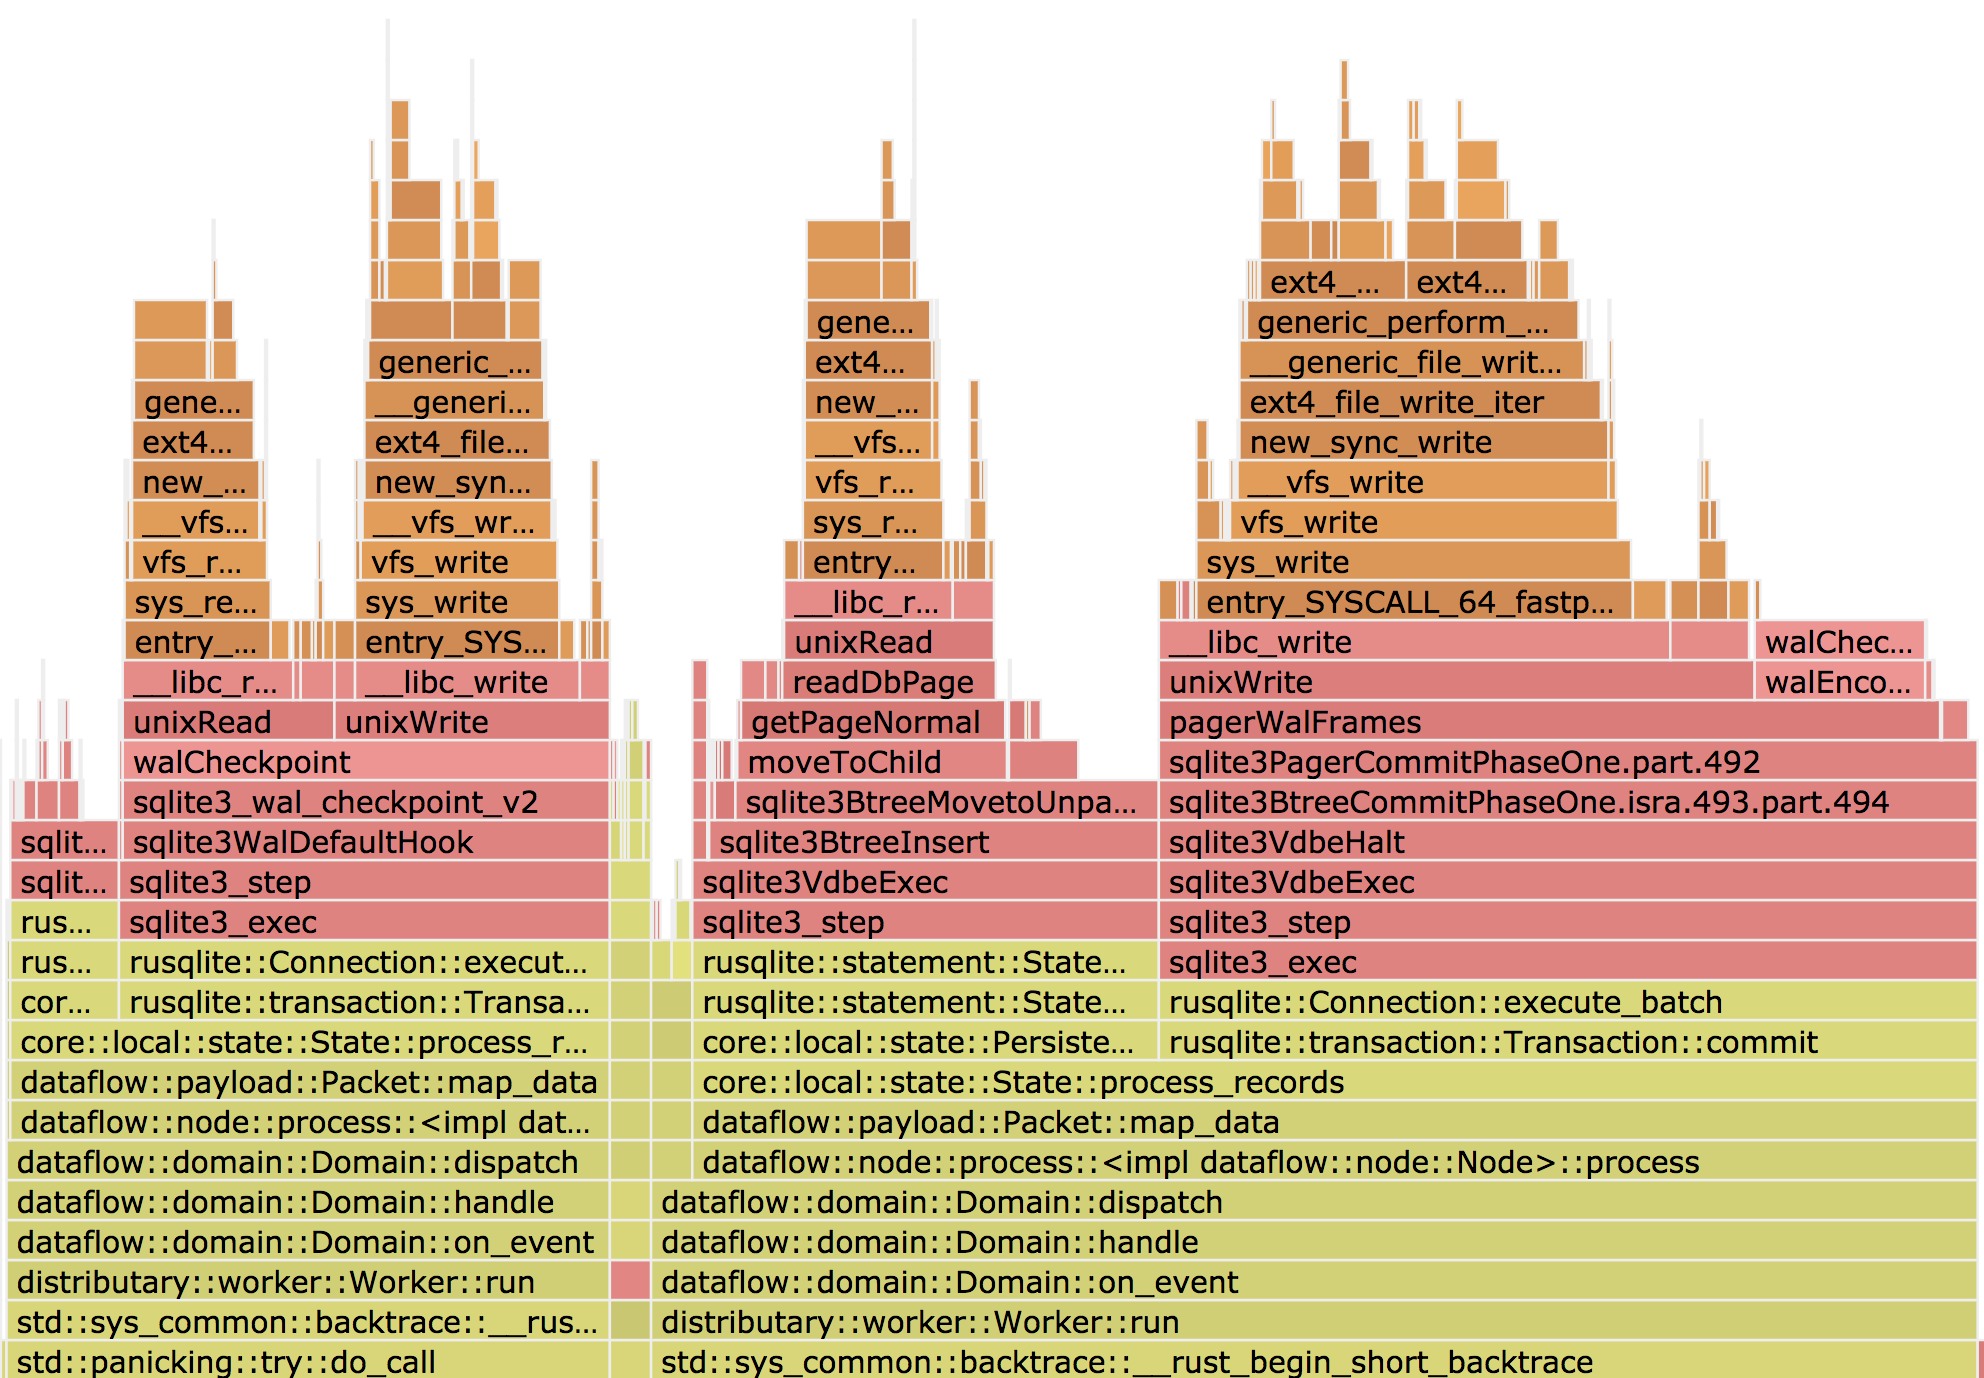
\includegraphics[width=\textwidth]{flame-example}
  \caption{\
    An example flame graph from events recorded using \code{perf}.
  }\label{fig:flame-example}
\end{figure}

\subsection{Memory}

% TODO: shitty sentence
Memory leaks happen when we continually allocate memory without freeing it. This
can easily happen in languages without dynamic memory allocation, when a
programmer forgets to deallocate some portion of memory after using it. At the
same time it can also happen in garbage collected languages, \eg when
continuously attaching listener functions to an event system without regard for
previous subscriptions. Rust's ownership system largely prevents issues of the
first kind from happening---variables that go out of scope are deallocated
automatically. Regardless, Rust supports calling into arbitrary C-programs (see
section~\ref{sec:ffi}), where anything could happen.

To profile memory leaks, the Valgrind
Massif\furl{http://valgrind.org/docs/manual/ms-manual.html} heap profiler is
used. Massif continuously takes snapshots of the heap, recording what memory is
used for, and where that memory was allocated from. While this is subject to
change in the future, current versions of Rust use the
\code{jemalloc}\furl{http://jemalloc.net/} memory allocator instead of the
system's default allocator. Unfortunately, memory profiling using Valgrind does
not work well with \code{jemalloc}. To resolve this we can instead force Rust to
use the system allocator, at least while profiling.

\begin{listing}[H]
  \begin{minted}[frame=lines]{rust}
#![feature(alloc_system)]
#![feature(global_allocator, allocator_api)]

#[global_allocator]
static ALLOC: std::alloc::System = std::alloc::System;
  \end{minted}

  \caption{Forcing Rust to use the system memory allocator makes it possible to
  profile it using tools such as Valgrind Massif.}\label{lst:system-alloc}
\end{listing}


\chapter{Related Work}\label{chap:related-work}

\chapter{Benchmarks}\label{chap:benchmarks}

Soup includes a series of benchmarks designed to reproduce different real world
scenarios where usage of Soup might be appropriate. The Lobsters and Vote
benchmarks existed prior to this thesis, while the Recovery and Replay
benchmarks were explicitly built to highlight the positive and negative impact
the features developed in this thesis have on Soup.

\newpage

\section{Hardware}

\subsection{Server setup 1: SSD}\label{sec:server-1}

Unless otherwise specified, benchmarks are run on Dell PowerEdge R430 server
with two Intel Xeon E5-2660 v3 CPUs and a total of 20 physical and 40 logical
cores. The server has 64GB of DDR4 RAM running at a speed of 2200MHz, with two
solid-state drives: a Samsung SSD 850 PRO and an Intel SSD S3710.

\subsection{Server setup 2: EC2 NVMe SSD}\label{sec:server-2}

Some of the benchmarks require the workload generator and clients to be
separated on a different machine than Soup itself. For these cases the
benchmarks are run on Amazon's Elastic Compute Cloud (EC2)
instances\furl{https://aws.amazon.com/ec2/instance-types/}, typically with the
workload generator running on a machine with a large number of cores and the
Soup server itself running on a server with fewer and faster cores.

When Soup needs access to fast durable storage, an \code{m4.10xlarge} is used
for the clients and an \code{i3.4xlarge} is used for the Soup workers. The
\code{m4.10xlarge} server uses an Intel Xeon E5-2686 CPU with 40 logical cores
and 160 GB of RAM.\@ The \code{i3.4xlarge} uses the same CPU as the \code{m4},
but is backed by NVMe SSDs capable of extremely high throughput I/O.

\subsection{Server setup 3: EC2 RAM Disk}\label{sec:server-3}

Similar to the setup in the previous section, the third setup makes use of two
servers hosted on Amazon EC2---this time without fast durable storage. Instead,
an \code{m5.12xlarge} and a \code{c5.4xlarge} is used. Both make use of newer
Intel Xeon Platinum processors, with 48 cores and 192GB RAM on the \code{m5} and
16 cores and 32GB RAM on the \code{c5}.

\section{Lobsters}\label{sec:lobsters}

Lobsters\furl{http://lobste.rs/} is a news aggregation website where users post,
vote and comment on links and discussions. Soup uses Lobsters to showcase the
performance advantages of Soup in a real-world application. While Lobsters is
built with Ruby on Rails, the Soup benchmark runs MySQL queries normally issued
by Lobsters directly against Soup, using the MySQL protocol shim described in
section~\ref{sec:mysql-shim}. This avoids the overhead of Ruby and Ruby on
Rails, which quickly become bottlenecks when the Lobsters traffic is scaled
beyond its regular workload.

Whereas the other benchmarks focus on individual writes and reads, the Lobsters
benchmark is measured in page views, where different pages execute a series of
write and read queries. The distribution of page views is modeled after real
Lobsters production traffic, to ensure the queries executed best resemble a real
Lobsters setup.

\begin{figure}[H]
  \centering
  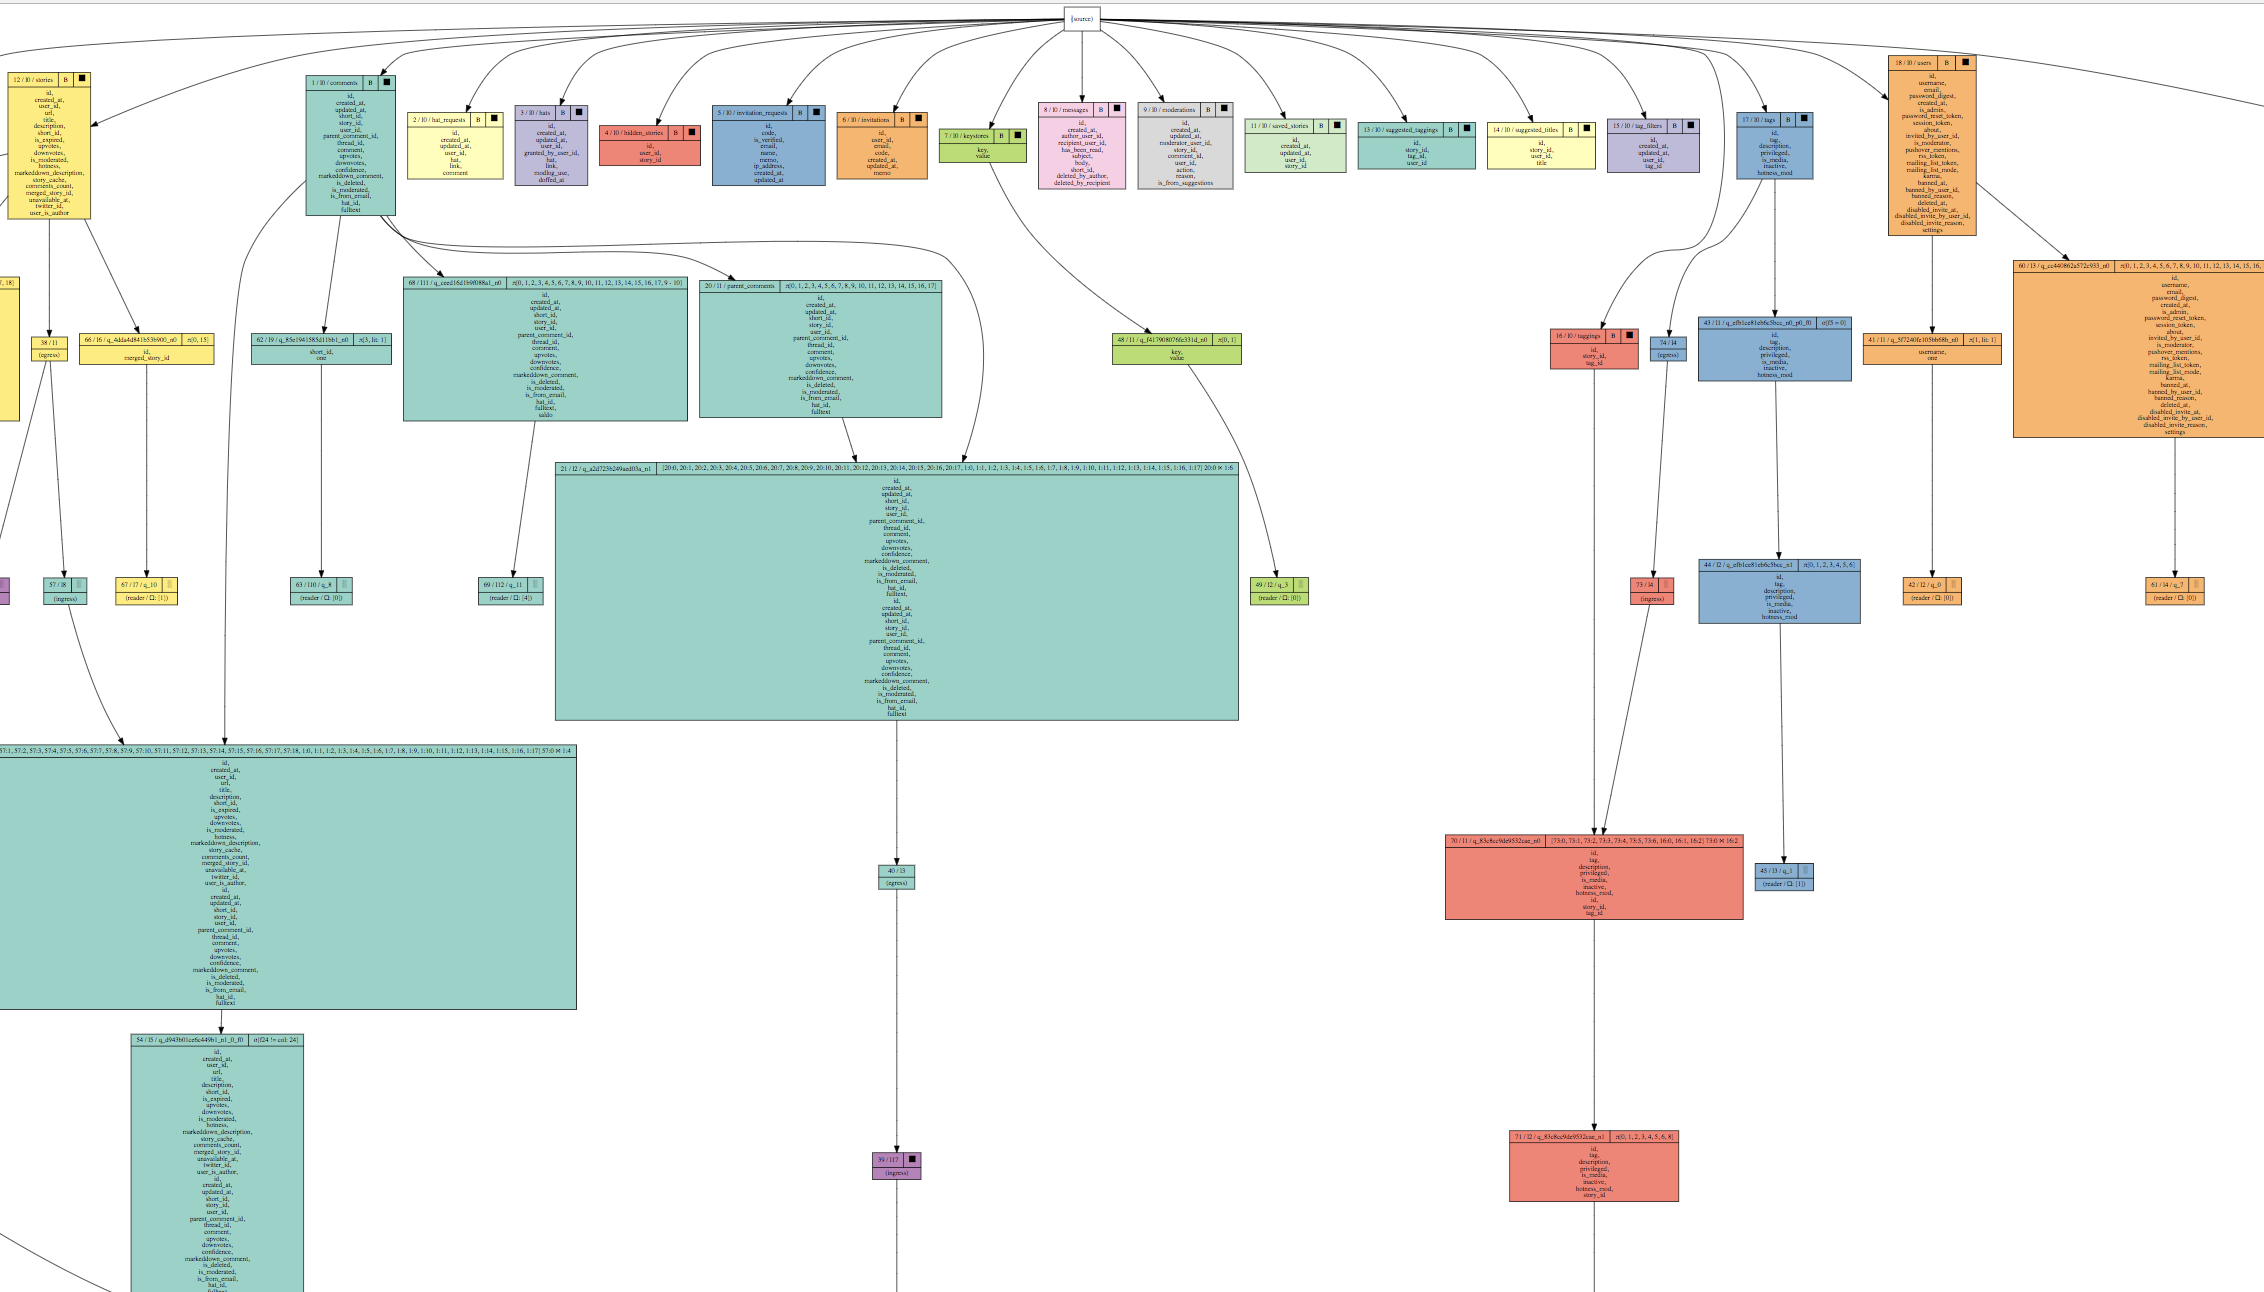
\includegraphics[width=\textwidth]{lobsters}
  \caption{\
    A subset of the Soup data-flow graph used to run the Lobsters benchmark.
  }\label{fig:lobsters-graph}
\end{figure}

The regular Lobsters queries rely on manual materializations and other
optimizations to reach decent performance using MySQL.\@ Part of Soup's goal is
to let developers write ``natural'' queries, without caching or other
denormalizing optimizations, and some of the Lobsters queries have been
rewritten to better highlight this.

\section{Vote}\label{sec:vote}

The Lobsters benchmark includes a wide variety of different queries, making it
difficult to narrow down bottlenecks in Soup's query processing performance. The
vote benchmark solves this by focusing on the most frequently run query in
Lobsters, reading stories and their corresponding vote counts.

\begin{listing}[H]
  \begin{minted}[frame=lines]{sql}
CREATE TABLE Article (id int, title varchar(255), PRIMARY KEY(id));
CREATE TABLE Vote (article_id int, user int);

QUERY ArticleWithVoteCount:
  SELECT Article.id, title, VoteCount.votes AS votes
  FROM Article
  LEFT JOIN (
    SELECT Vote.article_id, COUNT(user) AS votes
    FROM Vote
    GROUP BY Vote.article_id
  ) AS VoteCount
  ON (Article.id = VoteCount.article_id) WHERE Article.id = ?;
  \end{minted}

  \caption{The schema used by the vote benchmark.}\label{lst:vote}
\end{listing}

The database is prepopulated with a series of articles, letting the write
portion of the benchmark focus on writing votes, where each vote is assigned to
an article following a uniform distribution. The vote benchmark runs either
locally against a single Soup instance, or against a cluster of Soup workers.

\subsection{Open-loop}\label{sec:vote-open-loop}

In a closed-loop benchmark, a new request is issued when the previous completes.
With open-loop, requests are instead issued independently, resulting in a model
more closely resembling a real-world scenario~\cite{open-loop}. Soup's vote
benchmark relies on a \textit{partially} open-loop setup, where load is
generated by clients based on a specified distribution while maintaining a
capped queue of outstanding requests. This prevents reductions in measurements
during slower processing periods, where a closed-loop benchmark would issue far
fewer requests than an open-loop one.

Two latency measures are recorded during the vote benchmark: the time it takes
for a single batch to be processed (\textit{sojourn} time), and the time it
takes from the request is generated to it completes (\textit{batch processing}
time). The former is usually higher than the latter, as it includes the delay
from the request is queued until it is processed by the system.

\section{Replay}\label{sec:bench-replay}

Part of the promise of Soup is to avoid expensive computation when reading
queries, by moving most of the workload to the write portion of the system. Read
queries trigger replays for keys initially, while later reads are served
directly by partially materialized state later in the graph. This makes it
difficult to reason about the read performance of Soup's base nodes, as only a
small portion of reads are bound to be served by the base nodes at all.

This is where the replay benchmark comes in. Instead of possibly reading the
same keys multiple times, the replay benchmark ensures that each key is only
ever read \textit{once}, triggering a replay from the base nodes. Additionally,
the schema is far simpler than in the vote benchmark, with a single base node
and different variants of the same query. This is again done to further focus on
the base nodes, avoiding excessive computation in partial nodes down the graph.

\begin{listing}[H]
  \begin{minted}[frame=lines]{sql}
CREATE TABLE TableRow (
  id int, c1 int, c2 int, c3 int, c4 int,
  c5 int, c6 int, c7 int, c8 int, c9 int,
  PRIMARY KEY(id)
);

/* Primary key reads: */
QUERY ReadRow: SELECT * FROM TableRow WHERE id = ?;

/* Secondary key reads */
QUERY query_c1: SELECT * FROM TableRow WHERE c1 = ?;
/* .. */
QUERY query_c9: SELECT * FROM TableRow WHERE c9 = ?;
  \end{minted}

  \caption{The schema used by the replay benchmark.}\label{lst:replay}
\end{listing}

While trifling for the regular Soup base node implementation, the difference
between reading from a primary and secondary index might be consequential with
persistent base nodes (see section~\ref{sec:persistent-bases}). To correctly
assess this difference, the replay benchmark includes the possibility of reading
either from a primary or secondary index. The row size is also slightly larger
than in the other benchmarks, ensuring that the base nodes actually have to read
a fair share of data from state.

Prior to reading, Soup is populated with a given number of rows, which it then
reads a uniform, and smaller, sample of. With persistent Soup the benchmark
terminates after prepopulation, followed by a recovery step, to ensure that data
is served directly from durable storage. The file system cache is also cleared
after recovery and between subsequent benchmark runs.

\section{Recovery}\label{sec:bench-recovery}

The final benchmark measures the recovery time of our voting application, using
the schema described in listing~\ref{lst:vote}. The database is first populated
with a series of articles and votes, before being shut down and recovered from.

The benchmark produces two measures: initial and total recovery time. The former
records how long it takes for the first read to return correct data, while the
latter only finishes when up-to-date data is returned from \textit{all} keys.

\chapter{Persistent base nodes}\label{chap:persistent-bases}

Updates begin their journey through the Soup data-flow graph at the base nodes,
after being successfully persisted to Soup's write-ahead log. While nodes
further down in the graph might be \textit{partial}, the base nodes always
contain every single record a Soup application has seen through its lifetime.
This is crucial in maintaining a balance between efficient read queries and
space usage: popular queries will be handled by partial state further down the
graph, while reads for in-frequently accessed rows will be able to refer all the
way up to the source of truth, the base nodes, through what in Soup is called a
replay. In comparison to existing database systems, base nodes are closest to
what otherwise might be known as \textit{tables}.

\begin{figure}[H]
  \centering
  \includesvg[width=0.6\textwidth]{base-nodes}
  \caption{Updates enter the base nodes after being persisted to a write-ahead
  log.}
\end{figure}

While partial nodes can use \textit{eviction} (see~\ref{sec:eviction}) to keep
their memory footprint low, the size of base nodes will continue to grow
unbounded throughout a Soup instance's lifetime. In the short term this can be
handled by sharding Soup's data across multiple machines in a cluster, however
this is infeasible in the long term: sustained write workloads would continue to
grow the base node state, regardless of whether the data is accessed by queries
or not.

To combat this we would like to to move either parts of, or all of, the state
stored in base nodes to durable storage. This would reduce Soup's overall memory
usage, and perhaps even more significantly, transition Soup from a purely
in-memory database to a system that can store more data than its available
memory. With data safely persisted to base nodes, recovery after a failure would
also require less work, as partial nodes could gradually recover when data is
requested through replays. Summarized, introducing persistence to Soup's base
nodes would achieve the following goals:

\begin{enumerate}
  \item Prevent Soup's memory usage from growing unbounded over time
  \item Support larger-than-memory data sets
  \item Reduce recovery time after failures
\end{enumerate}

\newpage

\section{In-memory state}\label{sec:in-memory-state}

The current in-memory state implementation provides a key-value API with support
for multiple indices. A separate state data structure is kept for each
materialized node, including base nodes. The same data structure is used by both
partially and fully materialized nodes, but as base nodes always have to be
fully materialized, this section will omit describing details regarding the
former. The state data structure will be referred to as \code{State}.

\subsection{Adding indices}
The \code{State::add\_key} method introduces a new index to a specific \code{State} map,
and takes a set of columns as its argument. Additional indices do not lead to
multiple copies of the data, but rather contain pointers to the existing rows.
These pointers are held in separate data structures however: each new index
introduces a new hash map structure responsible for answering queries for that
specific set of columns.

New indices have to be \textbf{built}, as they are expected to answer queries
for data that has already been inserted, right away.

\begin{listing}[H]
  \begin{minted}[frame=lines]{python}
state = State()
// Initialize `state` with an index on the first column:
state.add_key([0])

// Then insert two rows:
state.insert([A, 1])
state.insert([B, 1])
assert_equal(state.lookup(A), [[A, 1]])

// Now, add an index on the second column:
state.add_key([1])
// ...which should return values that existed prior to the index being added:
assert_equal(state.lookup(1), [[A, 1], [B, 1]])
  \end{minted}

  \caption{Pseudo-code test that shows the expected behavior for adding indices
  with existing values.}\label{lst:existing-index}
\end{listing}

\subsection{Operations}

\subsubsection{Retrieval}

A stateful map would not be useful without a method for retrieving data, which
\code{State} provides through \code{State::lookup}. This takes a set of columns
and a key as its arguments, and make use of a \textbf{single} index to retrieve
one or more existing values. Each index is held in a separate hash map, and
retrievals can thus be completed in constant time.

That \code{State::lookup} can return more than one value is an important
distinction from most key-value stores, and is absolutely crucial in
implementing secondary indices. Without it \code{State} would only be able to
serve as an index structure for \textit{unique primary keys}.

\subsubsection{Insertion}

Naturally, to be able to read anything in the first place, we first need to
insert data into our stateful data structure. This is done through the
\code{State::insert} method, which takes a single row as its argument.
\code{State::insert} is responsible for updating every index in \code{State},
and has to loop through and insert a pointer for each included index.

\subsubsection{Removal}

Similar to insertions, removals have to update all indices. Contrary to what one
might expect, \code{State::remove} takes a single row as argument, and not a
key. This is due to how \code{State} is used in Soup: as an internal storage
unit for partially and fully materialized nodes alike. While it might make sense
for a base node to only delete rows by key, other nodes might need support for
deleting a single row, regardless of if its key is unique or not. No matter,
translating \code{remove(row)} to \code{remove(key)} is trivial, as shown in
listing~\ref{lst:removals}.

\begin{listing}[H]
  \begin{minted}[frame=lines]{python}
state = State()
state.add_key([0])
state.insert([A, 1])

row = state.lookup(A)
state.remove(row)
  \end{minted}

  \caption{Deleting a row from a base node in Soup.}\label{lst:removals}
\end{listing}

\subsubsection{Updates}
Similar to how \code{State} does not have a method for removing by key,
\code{State} does not include a method for updating a single row. Updates are
instead handled by the base node's logic, by first emitting a negative
record---to delete the existing row---followed by a positive one to insert the
new value.

\section{Requirements}\label{sec:requirements}
Random access memory is, and has been for years now, fast. Durable storage is
undergoing a similar transformation with the recent introduction of NVMe
SSDs~\cite{nvme}, but is still orders of magnitudes slower than RAM.\@ This
means that while introducing persistent storage into parts of the Soup equation
comes with many benefits, increased performance is not likely to be one of them.
Rather, the goal will be to maintain the existing performance characteristics,
while still achieving our three main goals.

\subsection{Write throughput}
Backfills of missing state, replays, go through the regular update paths in the
Soup data-flow graph. An increase in processing latency at the base nodes would
not only reduce the write throughput, but also have a significant impact on
reads that require a replay to complete.

\subsection{Point query performance}
Base node queries should be a seldom occurrence, as most queries should be
served by nodes further down the graph. Still, when a query eventually makes it
all the way up to the base nodes, it is important that it can be completed fast
enough to not significantly slow down the total read throughput of the system.
Slightly higher latency is on the other hand to be expected, we are after all
comparing persistent storage to an in-memory hash map.

\subsection{Support both primary and secondary indices}
Similar to Soup's existing \code{State} implementation, a durable replacement
has to support mapping a single key to multiple values, \ie secondary indices.

\section{Embedding an existing storage engine}
On-disk data structures have wildly varying performance characteristics. A
B+tree (see~\ref{sec:btree}) might perform well on random reads, but get heavily
out-performed by an LSM-tree (see~\ref{sec:rocksdb}) on sequential writes. At
the same time, decades of changes in hardware research have broadened the field
even further. A new NVMe SSD is able to reach almost half a million random reads
per
second\furl{http://www.samsung.com/semiconductor/minisite/ssd/product/consumer/ssd960/},
whereas a traditional spinning disk barely scratches the surface of a
hundred\furl{https://www.symantec.com/connect/articles/getting-hang-iops-v13}.
This makes building data structures for durable storage non-trivial and time
consuming.

On the other hand, there is a plethora of existing, open-source, storage
backends available today. Similar to their underlying data structures, different
backends are built for different use cases, with different hardware in mind.
This provides an option to implementing data structures from scratch, by instead
making use of existing database systems to test performance assumptions, which
is exactly what this thesis will do: first using SQLite, and later using
RocksDB.\@

\subsection{State interface}\label{sec:trait}
Before diving into the individual \code{State} operations, we need to pave the
way for the possibility of even having two different state implementations: the
existing in-memory implementation, and the new persistent storage variant, from
here on referred to as \code{MemoryState} and \code{PersistentState}. This is
achieved by turning the existing \code{State} implementation into an
interface---a \textit{trait} in Rust---which would then be implemented by both
the \code{State} variants. This helps maintain the current status quo where
\code{State} is an \textit{abstract data type}: internal Soup callers do not
need to be aware of the location their data is getting stored---they can simply
interact with the \code{State} trait as a black box\@.

\begin{listing}[H]
  \begin{minted}[frame=lines]{rust}
pub trait State {
    /// Add an index keyed by the given columns.
    fn add_key(&mut self, columns: &[usize]);

    /// Inserts or removes each record into State
    fn process_records(&mut self, records: &Records);

    /// Retrieve values from the index defined for `columns`.
    fn lookup<'a>(
      &'a self,
      columns: &[usize],
      key: &KeyType
    ) -> LookupResult<'a>;

    /// Count the rows currently stored in `State`.
    fn rows(&self) -> usize;

    /// Return a copy of all records.
    fn cloned_records(&self) -> Vec<Vec<DataType>>;
}
  \end{minted}

  \caption{\
    A segment of the main methods defined in our \code{State} trait.
  }\label{lst:state}
\end{listing}

As code is often more succinct than prose, a subset of the \code{State} trait is
shown in listing~\ref{lst:state}. The rest of the methods have been omitted for
clarity, as they are only relevant to nodes that can be partially
materialized---not base nodes. Similarly, some of the methods take in extra
arguments related to partial state---omitted here.

Comparing the trait in listing~\ref{lst:state} to the operations described
in~\ref{sec:in-memory-state} you might notice that the insert and removal
operations are gone. These have been abstracted into a higher level method:
\code{process\_records}. Every packet in Soup has the potential to contain more
than one record by being a merged packet, due to \textit{group commit}
(see~\ref{sec:group-commit}). Because of this, the function responsible for
materializing records in a node's \code{State} would go through a packet's
records, individually calling methods like \code{State::insert} and
\code{State::remove}. This is completely valid for an in-memory implementation,
where each operation has the same cost---without any initial overhead. This is
not the case for writes to potentially slower, durable storage. Here batching is
key, and an indicator to the underlying methods that they can perform operations
in one go is crucial.

\subsection{Ownership of data from \code{State}}
While other languages might implement memory safety through garbage collection
or manual memory management, Rust does the same through ownership, as described
in~\ref{sec:rust}. Whenever a value goes out of scope, it is deallocated. How
do you know when a value goes out of scope? In a garbage collected system, this
happens when there are no longer any references to the value. In Rust, each
value only has one owner, and any references need to live \textbf{at least} as
long as the value created by that owner.

However, what if a value needs to be owned by more than one location? That is
often the case for data structures, and \code{State} is no exception here.
Values stored in \code{MemoryState} should not have to be cloned during
retrieval, which would incur a heavy performance penalty. Instead, retrieving
values from \code{State} return dynamically reference
counted\furl{https://doc.rust-lang.org/std/rc/index.html} values,
allowing shared ownership of a single value by counting owners at runtime.
Subsequent retrievals of the same value always point to the same memory
location, with the source of truth being stored in \code{State}.

\todo{add a figure showing the difference between retrieving rows from memory
and from durable storage}

What if, on the other hand, a row does not exist in memory to begin with? This
would be the case when data is retrieved from durable storage: after reading a
row in its on-disk representation and de-serializing it to a value in Soup's
data format, where is that very value stored? The \textit{data} used to create
the value exists on disk, but the actual memory representation of the value was
just created. While \code{MemoryState::lookup} would want to return a reference
to an internally stored value, \code{PersistentState::lookup} would rather want
to hand over ownership of the value to the caller. Enter the
\code{Cow}\furl{https://doc.rust-lang.org/std/borrow/enum.Cow.html}
---a \textbf{clone-on-write} pointer from Rust's standard library that helps
with this exact purpose, by allowing data to be represented either as
\code{Borrowed} in the case of \code{MemoryState} or \code{Owned} for
\code{PersistentState}.

Additionally, the rows returned from \code{State::lookup} are wrapped in a
\code{LookupResult} enum, representing either a found or a missing value. The
latter is never relevant for \code{PersistentState}, which is only used to
represent fully materialized state. Note that a \textit{miss} does not signify
that the value does not exist, it simply means that this particular \code{State}
does not have it, while a \code{State} instance further up the data-flow graph
does.

\begin{listing}[H]
  \begin{minted}[frame=lines]{rust}
// Before:
pub enum LookupResult<'a> {
    Some(&'a [Rc<Vec<DataType>>]),
    Missing,
}

// After:
pub enum RecordResult<'a> {
    Borrowed(&'a [Rc<Vec<DataType>>]),
    Owned(Vec<Vec<DataType>>),
}

pub enum LookupResult<'a> {
    Some(RecordResult<'a>),
    Missing,
}
  \end{minted}
  \caption{\
    Prior to the introduction of \code{PersistentState}, reads from \code{State}
    would always result in a borrowed, reference counted value. Now that only
    happens for reads from \code{MemoryState}---with \code{PersistentState} the
    caller is responsible for retaining ownership of the value.
  }\label{lst:existing-index}
\end{listing}

\subsubsection{Using \code{LookupResult}}
Introducing the potential of a returned row being either \code{Borrowed} or
\code{Owned} has its downsides. For one, callers would have to handle both
branches, as the \textit{type} contained in a borrowed value is different from
the \textit{type} in an owned one. In the former, callers would always have to
clone the value to hand it over to someone else, whereas in the latter, they
could simply \textit{move} it out. The difference here comes from the
expectations of the value: a borrowed value implies that someone wants to retain
ownership of it---\eg it has to be cloned to give ownership to someone
else---while an owned value is the responsibility of the caller.

\begin{listing}[H]
  \begin{minted}[frame=lines]{rust}
if rows.len() > 0 {
  match rows {
    RecordResult::Owned(mut rows) => {
      out.push(Record::Negative(rows.swap_remove(0)))
    }
    RecordResult::Borrowed(rows) => {
      out.push(Record::Negative((*rows[0]).clone()))
    }
  }
}
  \end{minted}
  \caption{\
    With \code{RecordResult}, returned values can be either \code{Borrowed} or
    \code{Owned}, making callers responsible for handling both use cases. Here
    a negative record---used to signal to descendant nodes that this value
    should be invalidated---is emitted using the first row as its value.
  }\label{lst:cow}
\end{listing}

As is often the case, this can be simplified by looking at what the callers are
actually using the returned values for. The unpacked \code{rows} variable in
listing~\ref{lst:cow} is---as the name implies---a list of rows. Taking this
collection, and \textit{iterating} over either all of, or a subset of, the rows,
before returning a new iterator over the potentially modified values, was by far
the most common operation. Instead of delegating the responsibility for doing so
to the callers, this can be implemented on \code{RecordResult} itself, greatly
simplifying use cases like listing~\ref{lst:cow}.

\begin{listing}[H]
  \begin{minted}[frame=lines]{rust}
if let Some(row) = rows.into_iter().next() {
    out.push(Record::Negative(row.into_owned()));
}
  \end{minted}
  \caption{\
    The option of turning a \code{RecordResult} into an iterator is used to
    simplify the logic from listing~\ref{lst:cow}.
  }\label{lst:cow-better}
\end{listing}

\todo{write about IntoIterator and how it yields cows.} \\
\todo{include a more formal specification of how this works?}

\section{Persistent state with SQLite}
The first iteration towards a durable state implementation uses SQLite as its
storage engine. Described in section~\ref{sec:sqlite}, SQLite is a well-tested,
heavily used system with a track record in everything from applications to other
databases. SQLite uses B+trees internally---a reasonable, no frills data
structure with easy-to-reason about performance guarantees. This makes it useful
for a first prototype, and will help us answering the question of whether a
B+tree based \code{PersistentState} is feasible following the requirements
defined in~\ref{sec:requirements}. We will use the Rusqlite~\cite{rusqlite}
library for calling into SQLite from Rust.

\subsection{Schema}

SQLite is an embedded database, and requires no inter-process communication to
function. When persisting data, SQLite writes directly to durable files. This
requires exclusive locks to be held while writing (see~\ref{sec:sqlite-locks}),
eliminating the possibility of simultaneous updates from parallel locations to
the same database. This is not an issue for Soup and \code{PersistentState}.
Soup's \code{State} instances are completely standalone, and each
\code{PersistentState} instance can operate against a separate SQLite database,
avoiding the need for locks altogether.

SQLite---like SQL databases in general---require a strict schema to be defined
at all times. How this schema looks is usually a result of what kind of queries
a database needs to respond to, which in Soup's case depends on the indices a
specific \code{State} instance has been given responsibility for. Each column in
a Soup index will be given a column in the SQLite table, allowing flexible read
queries on any of the given indices. The row itself will be stored in a separate
column, serialized using \code{bincode} (see~\ref{sec:bincode}).

\subsection{Adding indices}

Each call to \code{State::add\_key} sets up that specific \code{State} instance
for queries on the given set of columns. This primarily involves extending our
SQLite schema with the newly given columns, while creating an actual SQLite
index on the \textit{column combination} itself. The latter is not strictly
necessary: SQLite is able to retrieve data for any columns, regardless of
existing indices. The performance would be exceedingly poor however, as it would
require scanning the entire table.

As an example, consider a Soup base node with the three columns \code{(a, b,
c)}. Queries further down the graph dictate that the base node needs to be able
to efficiently read rows by the columns \code{(a, b)}, and by only \code{c}.
After a series of inserts, our SQLite table for the base node's
\code{PersistentState} might look something like table~\ref{table:sqlite}.

\begin{table}[H]
  \centering
  \begin{tabular}{l l l l}
    \toprule
    \textbf{\code{a}} & \textbf{\code{b}} & \textbf{\code{c}} & \textbf{\code{row}} \\ \midrule
    1 & cat & norway & \code{bincode(1, cat, norway)}   \\ \midrule
    2 & dog & sweden & \code{bincode(2, dog, sweden)}   \\ \midrule
    3 & fish & denmark & \code{bincode(3, fish, denmark)} \\ \bottomrule
  \end{tabular}

  \caption{\
    An underlying SQLite table in \code{PersistentStore} after a few inserts.
    \code{bincode()} is used to signify that the value is serialized in the
    bincode binary serialization format.
  }\label{table:sqlite}
\end{table}

\subsection{Operations}

\subsubsection{Retrieval}

After the hard work of building the indices has completed, a myriad of rows is
only a \code{SELECT}-statement away. \code{PersistentState::lookup} takes a set
of columns and values for those columns as arguments, which are then translated
a \code{SELECT}-query. Considering the example in our previous section, the key
\code{(1, cat)} for the columns \code{(a, b)} would result in a query on the
form of \code{SELECT row FROM store WHERE index\_0 = 1 AND index\_1 = "cat"},
which SQLite can then complete in a timely manner due to the index on \code{(a,
b)}.

\subsubsection{Insertion}

Given a vector of values, \code{PersistentState} has to first extract the
columns necessary for its current set of indices and so that their values can be
translated to SQLite friendly types. These can then be used to build an
\code{INSERT}-query on the form of \code{INSERT INTO store (index\_0, index\_1,
row) VALUES (\ldots)}, where \code{row} is a binary representation of the entire
vector, serialized using \code{bincode}.

\subsubsection{Removal}

Similar to lookups, removals need to first build a \code{WHERE}-clause by
extracting the index column values from the target row, which can then be used
to perform a \code{DELETE}-statement on the form of \code{DELETE FROM store
WHERE index\_0 = 1 AND index\_1 = "cat"}.

\subsubsection{Processing insertions and removals}

All mutations need to be done within a transaction in SQLite, and operations
performed without an explicit transactions are implicitly given one. Performing
a single transaction is potentially expensive in SQLite, especially with strong
durability guarantees, where each transaction will incur a \code{fsync}
operation to make sure updates are successfully persisted before returning.

Instead, \code{PersistentState} batches all mutations required for a single
packet (per base node) into one transaction. This is done using the
\code{State::process\_records} method described in~\ref{sec:trait}, as shown in
listing~\ref{sec:process-sqlite}.

\begin{listing}[H]
  \begin{minted}[frame=lines]{rust}
fn process_records(&mut self, records: &Records) {
    let transaction = self.connection.transaction().unwrap();
    for r in records.iter() {
        match *r {
            Record::Positive(ref r) => {
                Self::insert(r.clone(), &self.indices, &transaction);
            }
            Record::Negative(ref r) => {
                Self::remove(r, &self.indices, &transaction);
            }
        }
    }

    transaction.commit().unwrap();
}
  \end{minted}

  \caption{Multiple insertions and removals are wrapped in a transaction.}\label{lst:process-sqlite}
\end{listing}


\subsubsection{Counting rows}

An accurate count of the total rows in the database can be retrieved using an
SQL \code{COUNT}-query: \code{SELECT COUNT(row) FROM store}.

\subsection{Replacing the Soup write-ahead log}\label{sec:sqlite-vs-soup}

Soup already writes all updates to durable storage in the form of a write-ahead
log. After an unexpected failure, Soup replays entries in the log to recover its
state to what it was prior to crashing. This is far from optimal for long
running applications (which most databases are), where recovery time would
simply continue to grow unbounded. Relying on SQLite for durability would let
Soup recover directly from SQLite's database files---a much faster operation
than replaying the entire log.

Modern SQLite versions make use of a write-ahead log to ensure durability
(see~\ref{sec:sqlite-wal}) while maintaining high write performance. Relying on
SQLite's WAL instead of Soup's requires some refactoring however: up until now
Soup has sent out acknowledgments of writes as soon as the write is merged into
a batch by the group commit protocol, prior to inserting the packet itself into
Soup's data flow graph. Materialization into \code{PersistentState} happens
after this on the other hand, while the packet is being processed by a base
node. This comes with a minor write latency penalty regardless of the
\code{State} implementation, as more work needs to happen before an
acknowledgment can be sent.

\begin{figure}[H]
  \centering
  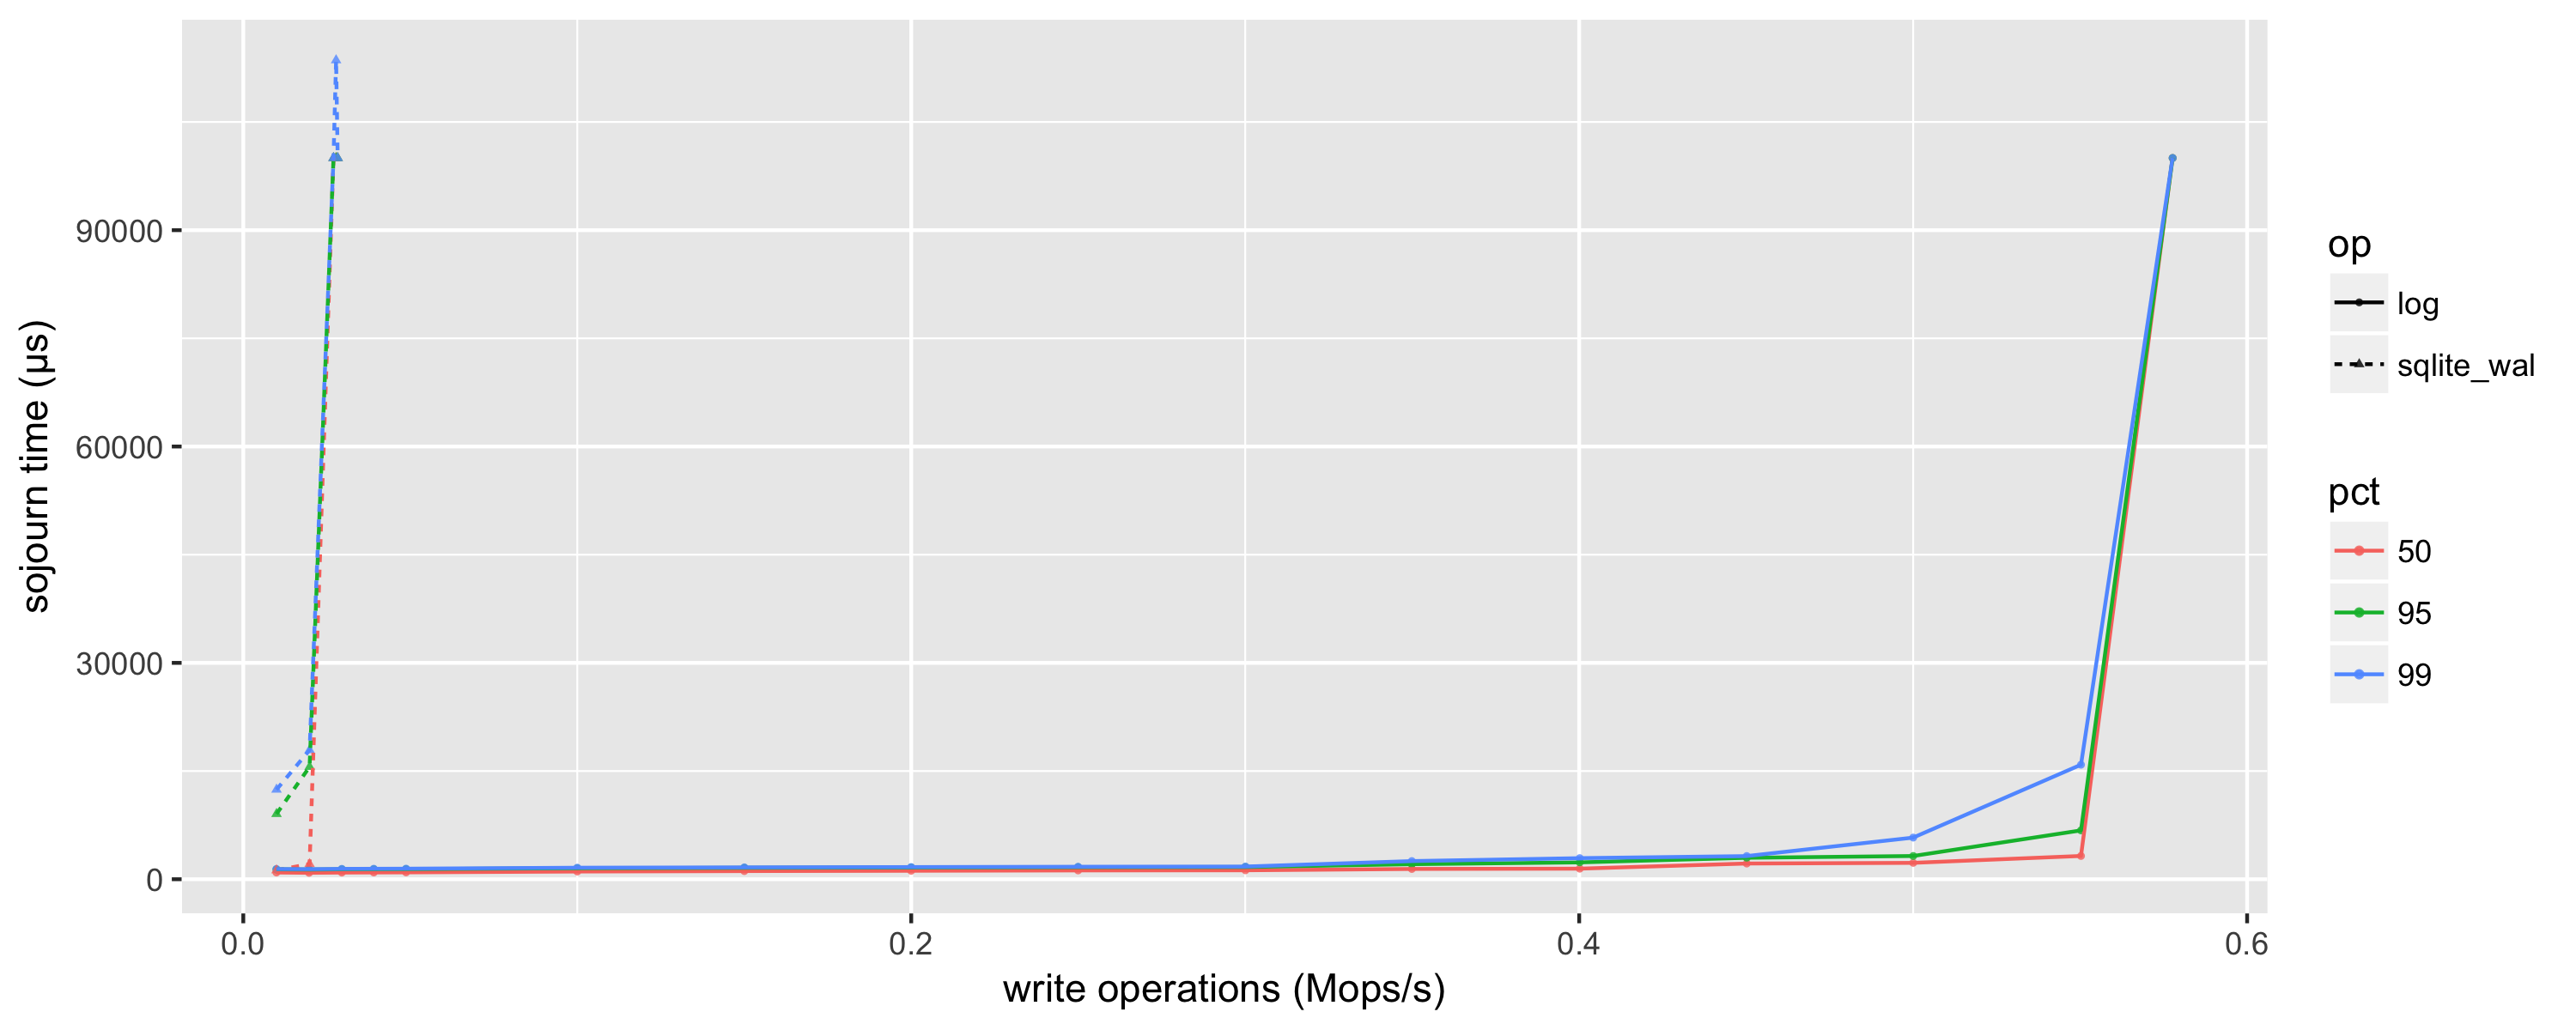
\includegraphics[width=\textwidth]{graphs/sqlite-wal-sjrn}
  \caption{\
    Write-only throughput measured using the \code{vote} benchmark. \code{log}
    relies on Soup's WAL for durability and stores base node state in-memory.
    \code{sqlite\_wal} uses SQLite for durability, storing all base node state
    on persistent storage.
  }\label{graph:sqlite-wal}
\end{figure}

Intuitively, one might expect writes to SQLite to be at least somewhat slower
than writes to Soup's regular write-ahead log, simply from the fact that the
latter needs to write less data to disk. At the same time, the WAL
implementation in SQLite is surely far more sophisticated than Soup's. SQLite's
WAL consists of a series of frames, allocated ahead of time to avoid unnecessary
resizing at every insertion. Soup's WAL is on the other hand purely an
ever-growing sequential file, where entries are appended to the end of the file
for each new packet. So why---as shown in figure~\ref{graph:sqlite-wal}---is
SQLite so much slower?

\subsubsection{Checkpointing}

With an arsenal of profiling tools at our disposal, guessing is unnecessary. A
flame graph built from profiling data recorded with \code{perf} quickly
highlights the two main culprits: checkpoints and B-tree updates. As mentioned
in section~\ref{sec:sqlite-checkpoints}, SQLite automatically transfers data
from the WAL to its main database file once the WAL exceeds a certain threshold.
Checkpointing---similar to everything else in SQLite---is a synchronous
operation, incurring a significant latency penalty once it happens. Regardless,
checkpointing is a necessary evil. Up until the point of a checkpoint, reads
have to refer to both the content in the WAL and the content in the main
database. Delaying the automatic checkpoint operation does not make much of a
difference either, as it results in more content to copy over when the
checkpoint finally occurs.

\begin{figure}[H]
  \centering
  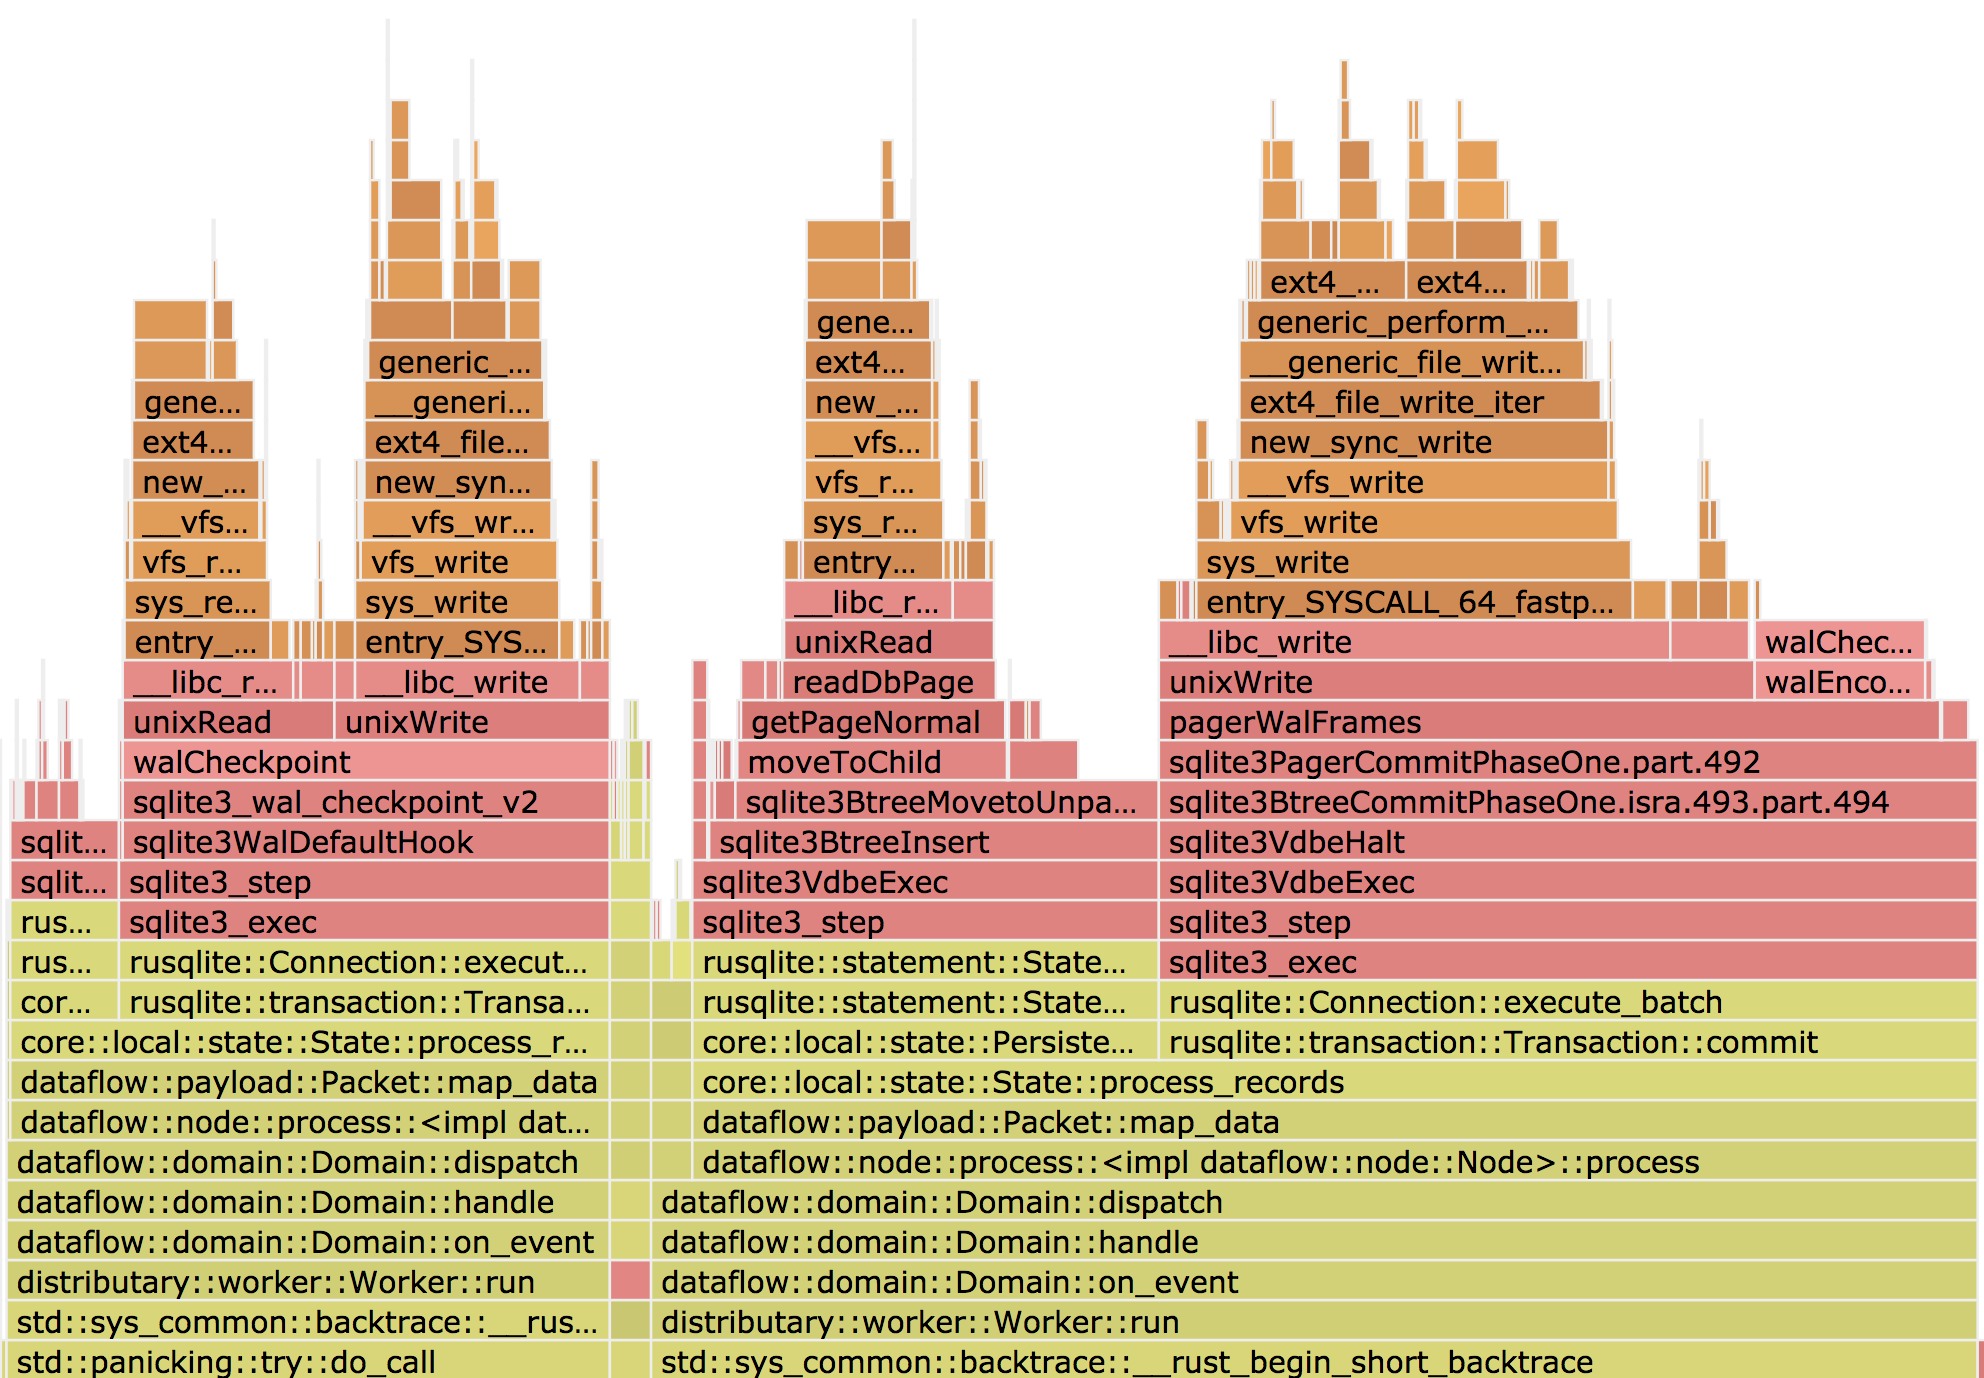
\includegraphics[width=\textwidth]{sqlite-wal-flame}
  \caption{A flame graph highlighting time consuming functions in
  \code{PersistentState}.}\label{fig:sqlite-wal}
\end{figure}

Does checkpoints have to happen synchronously, before a write acknowledgment is
sent to a client? In reality, they do not: taking a checkpoint does not make any
difference in terms of durability. Instead, \code{PersistentState} can issue a
checkpoint manually after a certain amount of time, but \textit{after}
acknowledging any outstanding writes. This had a minor effect on throughput,
taking it from a measly 27k ops/s, to at least 42k ops/s---still far too slow.
The checkpoints still happen synchronously, pausing processing at that specific
\code{PersistentState} instance for a significant amount of time instance for a
significant amount of time.

That leads to the question of whether checkpoints have to happen in the same
thread as regular processing altogether. The SQLite manual mentions the
possibility of taking checkpoints in a separate thread, by incurring manual
checkpoints using the \\ \code{sqlite3\_wal\_checkpoint\_v2} API.\@ While this
sounds promising, it only helps if regular processing can continue while the
checkpoint is being taken. SQLite describes four different checkpoint
modes\furl{https://www.sqlite.org/c3ref/wal_checkpoint_v2.html}:

\begin{itemize}
  \item \code{SQLITE\_CHECKPOINT\_PASSIVE}: Checkpoints as many frames as
    possible without taking any locks.
  \item \code{SQLITE\_CHECKPOINT\_FULL}: Wait until any current database
    operations are finished, then hold an exclusive write-lock while
    checkpointing.
  \item \code{SQLITE\_CHECKPOINT\_RESTART}: Similar to the previous mode, but
    waits with finishing the checkpoint until all readers are accessing the
    main database file---and not the WAL---forcing any new writers to restart
    the WAL.\@
  \item \code{SQLITE\_CHECKPOINT\_TRUNCATE}: Same as the \code{RESTART} mode,
    except it also truncates the log file before restarting.
\end{itemize}

While the last three checkpoint modes hold write locks throughout the duration
of the checkpoint, effectively resulting in the same operation as a synchronous
checkpoint, the \code{PASSIVE} mode does not. It also has the possibility of not
checkpointing any frames whatsoever either though, which is not very helpful.
This makes it heavily workload dependent, as it requires a low enough throughput
to allow ``breaks'' in the write processing where a checkpoint can happen. Without
that being the case the WAL will simply continue to grow.

\subsubsection{Updating indices}

The other issue highlighted in the flame graph in
figure~\ref{fig:sqlite-wal} is index updates. While writing to a
write-ahead log is purely sequential, updating B-trees is not. This is a
significant difference from Soup's write-ahead log, where writes to the log only
require sequential writes, instead of the random reads \textbf{and} writes
caused by inserting into a B-tree. Even if maintaining SQLite's B-tree indices
could be postponed to the checkpoint stage (which would likely degrade read
performance), this would simply lead to a longer checkpoint, which, as the
previous section points out, still results in pauses in regular write
processing.

\subsection{Relaxing SQLite's durability guarantees}

To ensure durability, SQLite waits until writes have been fully persisted to
durable storage before returning. Depending on the underlying storage medium,
this might come with a quite hefty latency penalty, as the previous sections
have shown. Let us now move to the other end of the spectrum, and investigate
how SQLite fares with minimal durability guarantees. Instead, we will rely on
Soup's regular write-ahead log for durability, and only use SQLite to avoid
having to store base node state in memory.

\subsubsection{Synchronization}

Whereas the previous experiments ran with SQLite's \code{synchronous} option set
to \code{FULL}---which ensures that all writes are safely persisted before
returning---we will now make use of \code{synchronous = OFF} instead, which
should significantly decrease write latency to SQLite.

\subsubsection{Foregoing atomicity}

SQLite provides two main options to ensure atomicity: a rollback journal
(section~\ref{sec:sqlite-locks}) and a write-ahead log
(section~\ref{sec:sqlite-wal}). Whereas the previous section made use of the
latter, we will now try a third option: no journal at all. Similar to
\code{synchronous = OFF} this is far from safe in the event of crashing, but
is altogether a more useful comparison while relying on Soup's WAL for
durability. If this is still too slow, then chances are it is going to be hard
to achieve our predefined requirements using SQLite no matter what.

\subsubsection{Results}

Whereas our SQLite WAL experiment only reached about 40k writes/s, the current
setup is at least able to push past 110k writes/s. While an improvement, this
is still far slower than Soup's regular write-ahead log.

\begin{figure}[H]
  \centering
  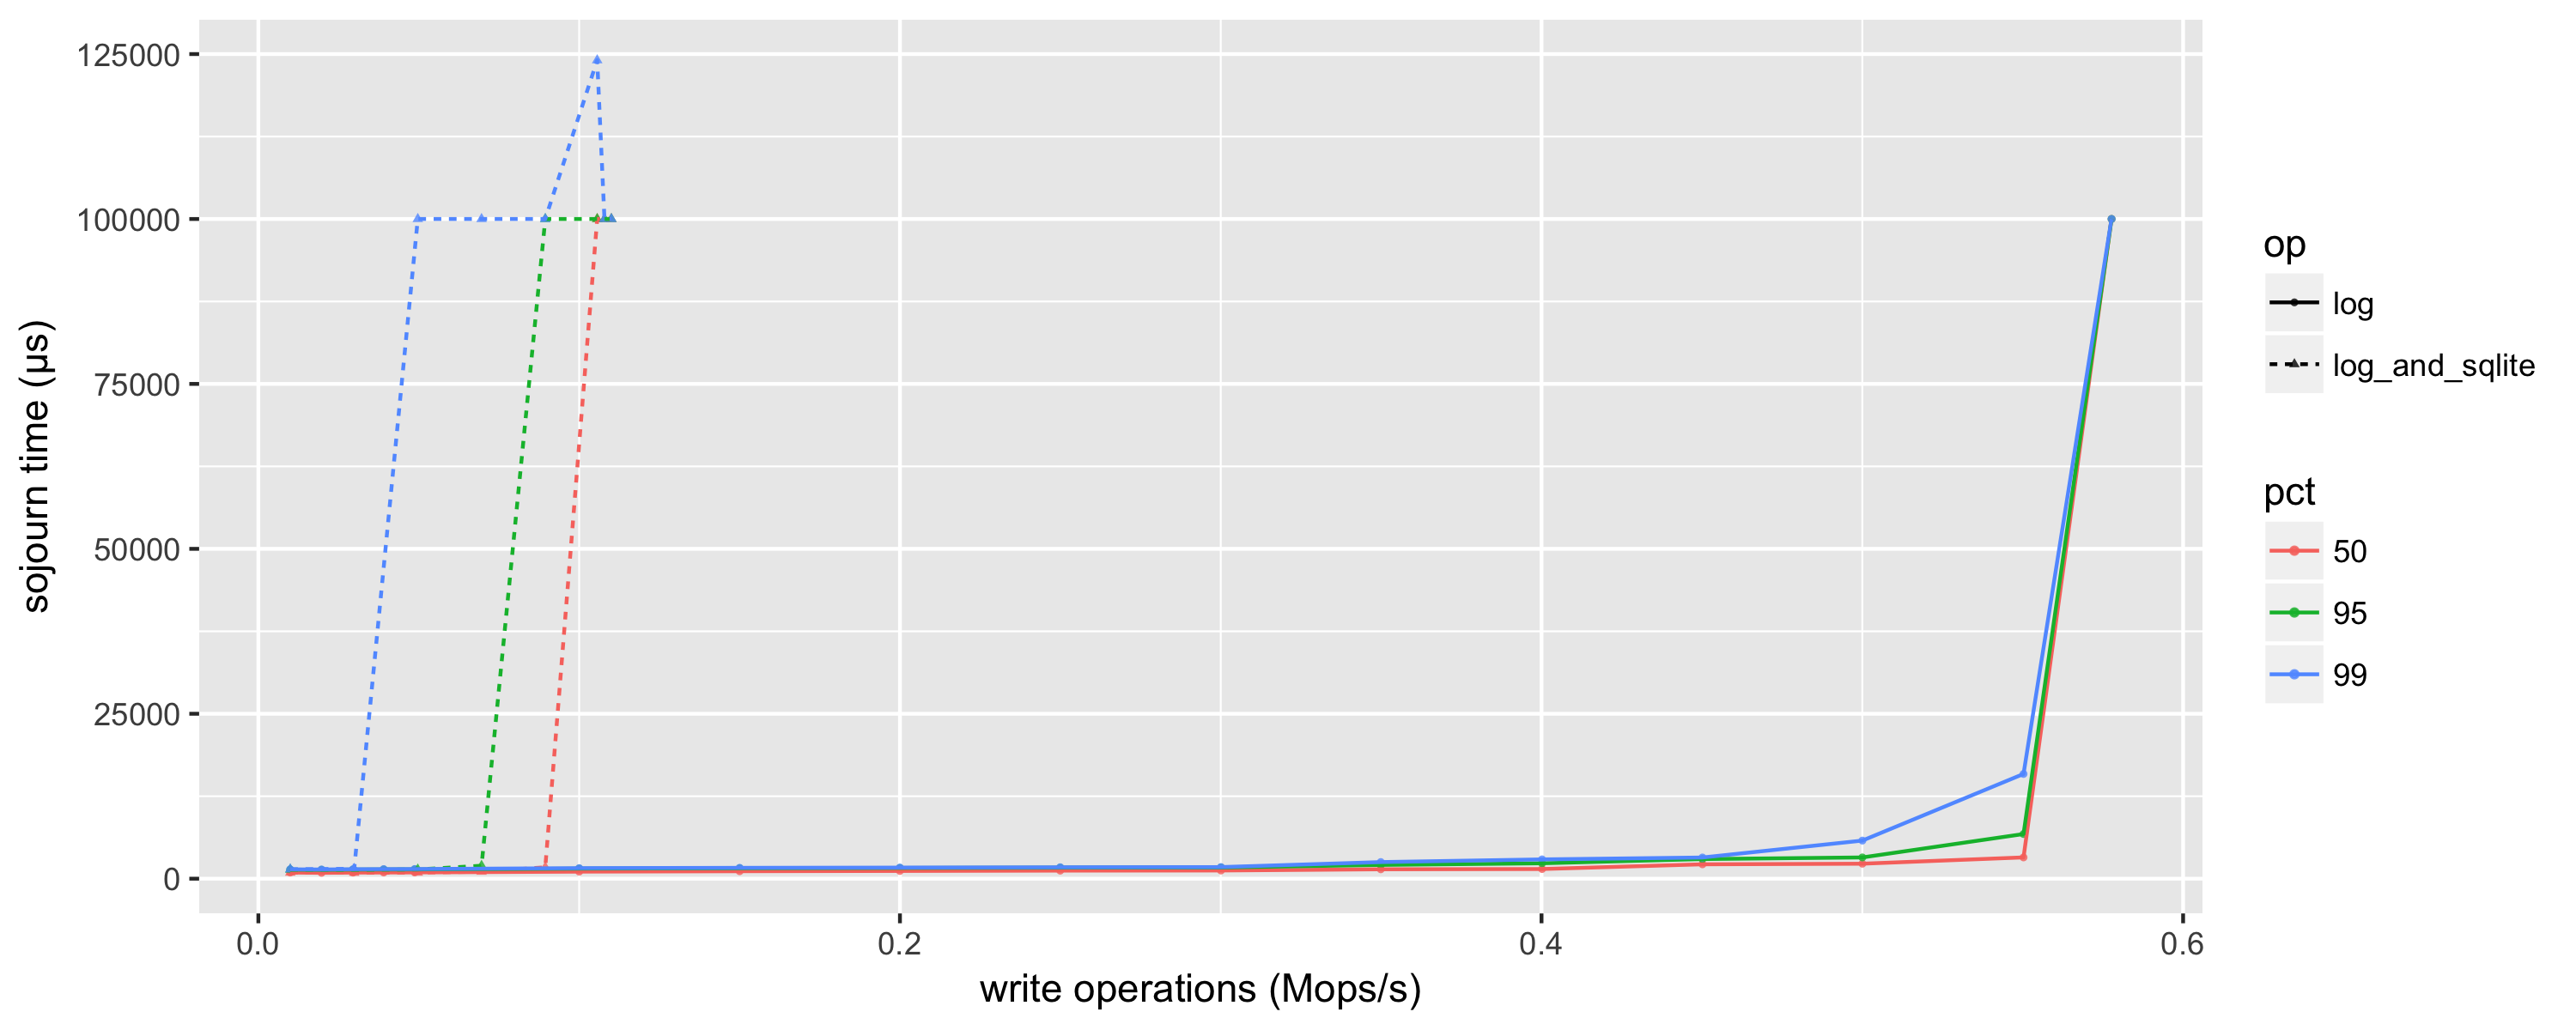
\includegraphics[width=\textwidth]{graphs/sqlite-soup-log}
  \caption{\
    Write-only throughput measured using the \code{vote} benchmark, comparing
    in-memory base nodes to persistent base nodes using SQLite---both examples
    use Soup's WAL for durability.
  }\label{graph:sqlite-soup-log}
\end{figure}

\todo{could write about the (failed) attempt of batching more writes together}

\subsubsection{Closing remarks}

The fact that SQLite works well out of the box without a lot of tuning is
definitely one of its strengths. Regardless, there are a few options that can be
tweaked, both ahead of compilation and at runtime. While disabling SQLite
features not needed for \code{PersistentState} and removing all mutex code had a
slight positive impact, the improvements were far from significant enough to
make a solid dent in the total throughput.

Maintaining SQLite indices---and thus randomly reading from and writing to
disk---on the main path is simply too slow. Does this imply that directly
maintaining B-tree on-disk index structures built specifically for Soup would
perform poorly as well? Possibly. While SQLite does have a lot of overhead
needed to support a wide range of features, and an even wider array of systems,
profiling clearly shows that the bulk of processing time is spent interacting
with durable storage as a result of B-tree maintenance.

\section{Persistent state with RocksDB}

How do we improve upon SQLite's low write throughput? One option would be to
only write to durable storage from background threads, avoiding the hit in
latency that comes with writing to and reading from disk. Instead, writes to
\code{PersistentState} could fill up an in-memory queue structure, which would
then later be flushed to persistent storage by background threads. Read
operations could then retrieve data from both the in-memory queue and the
slower---but persistent---SQLite. This might sound familiar, as it is
effectively a naive sketch of the log-structured merge-tree data structure
described in section~\ref{sec:rocksdb}, where writes are initially kept in an
in-memory buffer and later flushed to disk by background workers. That leaves us
with a good next step: embedding a storage engine that makes use of LSM-trees
internally, RocksDB.\@

While RocksDB and its LSM-trees should improve \code{PersistentState}'s write
throughput, it could at the same time introduce a further penalty to read
latency. This might not be too problematic though, as reads from
\code{PersistentState} should be more of a rare occurrence than writes: every
update Soup sees needs to be persisted to durable storage, whereas only a subset
of reads need to access \code{PersistentState} at all---most results should be
served by partial nodes further down the data-flow graph.

\subsection{Secondary index scheme}

Whereas SQLite includes support for a large subset of SQL features, RocksDB's
API is on a lower abstraction level. Limited to the functions necessary to
maintain a sorted key-value store, implementing support for secondary indices is
more of a challenge than with SQLite, where support for both primary and
secondary indices is built in. Building higher level abstractions on top of
key-value stores is becoming more and more common however, with plenty of
inspiration to be found in existing projects. Both CockroachDB~\cite{cockroach}
and MyRocks~\cite{myrocks} implement SQL-like functionality on top of RocksDB,
with sturdy indexing schemes at the core.

Prior to describing the final implementation, let us first iterate our way
towards a working index scheme. The next few sections describe separate,
working, implementations, where each step improves upon the last.

\subsubsection{Collection of rows}

Representing unique indices using a key-value store is fairly straight forward,
as each key maps to a single value. With secondary indices, this is no longer
the case, and a single key would need to represent multiple values. With
key-value stores where subsequent insertions are still retrievable with a single
read operation this would require no further abstractions. In RocksDB however,
each insertion effectively overwrites any existing values that might exist for
that key. So how do we emulate an API mapping a single key to multiple values
with the tools we have at hand? For a start, we could do exactly that, and store
multiple values in an array below each key. Insertions would then retrieve the
array of existing values, append the given value to that array, and write it
back to the same key---as shown in listing~\ref{lst:collection-secondary}.

\begin{listing}[H]
  \begin{minted}[frame=lines]{python}
Lookup(key):
  raw_values = Get(key)
  deserialize(raw_values) or []

Insert(key, value):
  # Retrieve and deserialize existing values:
  raw_values = Get(key)
  values = deserialize(raw_values) or []

  # Append our new value, serialize the collection and put it back:
  values += value
  Put(key, serialize(values))
  \end{minted}

  \caption{A naive secondary index implementation, where each key contains a
  collection of values.}\label{lst:collection-secondary}
\end{listing}

Unfortunately, this comes with the same write performance penalty as SQLite's
B-tree index structures: each write now has to first perform a random read
\textit{before} the new value can be written. This completely removes any
performance benefits we might gain from RocksDB's write-friendly LSM-tree
structure.

\subsubsection{Merge operator}

In addition to the more common \code{Get} and \code{Put} operations, RocksDB
supports an atomic read-modify-write operation through the \code{Merge}
method\furl{https://github.com/facebook/rocksdb/wiki/Merge-Operator}.
This leads to the same result as in our previous implementation---with each key
mapping to a collection of values---without any random reads while writing.
Instead, RocksDB considers calls on the form \code{Merge(key, value)} as an
\textit{intent} to merge the values, and persists it as such. These intents can
then be processed later, during background compactions (see
section~\ref{sec:compactions}) and read operations.

\begin{listing}[H]
  \begin{minted}[frame=lines]{python}
Lookup(key):
  raw_values = Get(key)
  deserialize(raw_values) or []

MergeOperator(key, existing, operations):
  # Retrieve and deserialize existing values:
  values = deserialize(existing) or []

  # Then, append all Merge(key, value) operations:
  for op in operations
    values += deserialize(op)

  # Finally, serialize and return the new list:
  serialize(values)
  \end{minted}

  \caption{A RocksDB merge operator, appending any given values to an array.}\label{lst:merge-fn}
\end{listing}

This moves some of the work from writing to reading, as a read operation now has
to find all merge operands and process them before returning. Unfortunately,
this also introduces an unnecessary amount of serialization. RocksDB does not
know how to deal with anything but byte streams, and so both the input and
output to the merge operator has to be serialized, regardless of the fact that
the final result will have to be deserialized again when read by the caller.
This could potentially be improved through a smarter serialization scheme, where
values could be appended to the serialized array without deserialization, but
let us first consider an alternative without the merge operator altogether.

\subsubsection{Iteration}

Up until now we have considered options where each index value takes up a single
key, through various methods of making the value portion of a key-value pair
plural. This has shown to be quite sub-par, and it would certainly be an
improvement if we could avoid storing a collection below each key. This is
possible through \textit{iteration}. By varying keys slightly to ensure
uniqueness, while still making sure keys corresponding to the same index value
are placed next to each other, we can \textit{seek} to the first key for a
specific index value, and continue to iterate through its subsequent siblings
until we reach a separate key altogether. Retaining uniqueness among keys is not
completely straight forward, and while we will consider this in further detail
in section~\ref{sec:ensuring-uniqueness}, we we will for now make do with a
monotonically increasing sequence number, where each subsequent insertion
increments the sequence number and appends it to the original key.

Consider an example table with three columns and two indices: \code{(id, name,
country)}, with a primary index on \code{id} and a secondary index on
\code{country}. Table~\ref{table:iteration} shows how the structured schema is
converted to a flattened key-value space by inserting additional rows for each
index. Notice that the keys for the primary index do not need any additional
suffixes to ensure uniqueness---its keys are already considered unique among
each other.

\begin{table}[H]
  \centering
  \begin{tabular}{l l l}
    \toprule
    \textbf{id} & \textbf{name} & \textbf{country} \\ \midrule
    1 & ola & norway \\ \midrule
    2 & kari & norway \\ \bottomrule
  \end{tabular}
  \quad
  \begin{tabular}{l l}
    \toprule
    \textbf{key} & \textbf{value} \\ \midrule
    1 & (1, ola, norway) \\ \midrule
    2 & (2, kari, norway) \\ \midrule
    norway-1 & (1, ola, norway) \\ \midrule
    norway-2 & (2, kari, norway) \\ \bottomrule
  \end{tabular}

  \caption{\
    Flattening a structured table with multiple index into a key-value scheme.
  }\label{table:iteration}
\end{table}

\begin{listing}[H]
  \begin{minted}[frame=lines]{python}
Lookup(key):
  values = []
  iterator = Iterator()
  iterator.seek(key)
  while iterator.valid():
    (next_key, next_value) = deserialize(iterator.next())
    if not next_key.starts_with(key):
      break

    values += next_value

  values

Insert(key, value):
  seq++
  new_key = serialize(key + seq)
  Put(new_key, serialize(value))
  \end{minted}

  \caption{Implementing an indexing scheme using iteration.}\label{lst:iteration-example}
\end{listing}


\subsection{Prefix Iteration}\label{sec:prefix-iteration}

While iteration is a promising concept, the performance guarantees it provides
are potentially sub-par. Consider how an LSM-tree organizes its data: whereas
each SS-table is sorted, separate files often overlap. This implies that an
iterator has to consider every available file in its tree while iterating. To
improve upon this, we can provide RocksDB with a way of partitioning out the
areas that we want to iterate within, through use of \textit{prefix
extractors}. In our case, these partitions are separate index keys, such as
\code{norway} in the example shown in table~\ref{table:iteration}.

After defining a way of extracting these prefixes, RocksDB is free to organize
its data to optimize for prefix iteration. While previously guaranteeing a total
order among all keys, RocksDB now only does so within a prefix. Bloom filters
(see section~\ref{sec:bloom}) can then be defined on prefixes instead of
individual keys, greatly reducing the amount of SS-tables that have to be
considered when iterating. Additionally, developers can choose to replace
RocksDB's fundamental LSM-tree structures with data structures optimized for
prefix iteration, such as hash tables where each prefix is a key.

\subsubsection{Extracting a prefix}

What signifies a prefix varies wildly between different applications. Instead of
attempting a generalization, RocksDB leaves the extraction up to developers,
through what is referred to as a \textit{slice transform}: a function on the
form of $ S \rightarrow S' $, where $ S $ is a slice and $ S' $ is a potentially
modified version of $ S $. For \code{PersistentState}, $ S' $ corresponds to the
original key, with any appended suffixes stripped away, as shown in
table~\ref{table:prefix}.

\begin{table}[H]
  \centering
  \begin{tabular}{l l l}
    \toprule
    \textbf{key} & \textbf{prefix} & \textbf{value} \\ \midrule
    1 & 1 & (1, ola, norway) \\ \midrule
    2 & 1 & (2, kari, norway) \\ \midrule
    norway-1 & norway & (1, ola, norway) \\ \midrule
    norway-2 & norway & (2, kari, norway) \\ \midrule
  \end{tabular}

  \caption{\
    The extracted prefixes strip away the previously appended key suffixes.
  }\label{table:prefix}
\end{table}

This gives us the ability to iterate purely within a prefix. Instead of having
to manually check whether our next iteration step reaches a sibling key, we can
now seek directly to the prefix and RocksDB will ensure that all given keys
stays within that prefix. At the same time, we do not have to take care to make
sure that the first key---\eg \code{norway-1}---is ordered before any other
keys: RocksDB ensures that our prefix iterator steps through all keys within
that prefix. To define a correct prefix extractor, RocksDB defines four
boolean properties that need to hold:

\begin{enumerate}
  \item $ key.starts\_with(prefix(key)) $
  \item $ Compare(prefix(key), key) \leq 0 $
  \item $ Compare(k1, k2) \leq 0 \Longrightarrow Compare(prefix(k1), prefix(k2)) < 0 $
  \item $ prefix(prefix(key)) \equiv prefix(key) $
\end{enumerate}

Every key has to go through a defined slice transform at some point, so an
efficient implementation is crucial. This is not completely trivial though, as
both the prefix transform's input and output are byte streams. How do we
separate out the index part of a key from a byte stream? A naive way to do so
would be to first deserialize the key, extract the index values, before finally
serializing and returning the prefix in byte form (shown in
listing~\ref{lst:naive-prefix}).

\begin{listing}[H]
  \begin{minted}[frame=lines]{python}
PrefixTransform(raw_key):
  try:
    key, suffix = deserialize(raw_key)
  catch:
    # raw_key might already have gone through a prefix transform (property 4):
    return raw_key

  serialize(key)
  \end{minted}

  \caption{A naive implementation of a prefix transform.}\label{lst:naive-prefix}
\end{listing}

Deserializing the \textit{entire} key just to strip off the suffix requires an
unnecessary amount of allocations. In the current example the suffix is an
integer sequence number, which we always know the byte size off, giving us the
alternative of slicing away the last $ X $ bytes from the key to build a prefix.
This would help maintain the three first prefix transformation properties, while
failing the last: how do we ensure that we only slice away the last bytes once
when performing $ prefix(prefix(key)) $? Additionally, as we will see in later
sections, there are cases where we would like the suffix to have a variable byte
size.

This leaves us with a requirement for a more generic solution, which we will
solve by slightly worsening the space complexity of our key scheme, through the
introduction of a \textit{size} segment. Consider a 64-bit integer primary key $
X $, which bincode (see section~\ref{sec:bincode}) uses 12 bytes to serialize.
By prefixing the key with the serialized size, 12, the slice transform knows how
many bytes correspond to the index value of the key, which it can then use to
remove any suffix values.

\begin{listing}[H]
  \begin{minted}[frame=lines]{python}
PrefixTransform(raw_key):
  # bincode uses 8 bytes to encode
  # the size value itself, a 64-bit integer:
  size_offset = 8
  key_size = deserialize(raw_key[..size_offset])
  prefix_length = size_offset + key_size
  # Finally, strip away the suffix:
  raw_key[..prefix_length]
  \end{minted}

  \caption{\
    With the byte size of the relevant portion of the key included,
    \code{PrefixTransform} only needs to deserialize a single integer to be able
    to slice away the suffix.
  }\label{lst:better-prefix}
\end{listing}


\subsection{Separating indices}

The index scheme described so far has glossed over the potential for conflicts
between indices covering the same amount of columns, with the same types.
Consider a table with two integer columns---\code{(a, b)}---and an index on each
column. How do you separate values pointed to by the index on \code{a} from
values pointed to by the index on \code{b}? In the example shown in
table~\ref{table:colliding} this would lead to a conflict: both index \code{a}
and index \code{b} have at least one key with the same value.

\begin{table}[H]
  \centering
  \begin{tabular}{l l}
    \toprule
    \textbf{a} & \textbf{b} \\ \midrule
    1 & 2 \\ \midrule
    2 & 2 \\ \midrule
  \end{tabular}

  \caption{Two indices with the same number and type of columns would collide
  under a flat key-value space.}\label{table:colliding}
\end{table}

Both CockroachDB~\cite{cockroach-encoding} and MyRocks~\cite{myrocks-encoding}
solve this by including a unique index ID in the key (shown in
table~\ref{table:index-id}). This is an elegant solution with low overhead---a
small integer value would be enough to cover a large amount of indices. Another
option would be to put each index in a separate column family---the RocksDB
equivalent of a table. Whereas a secondary index might have a large amount of
values prefix, a unique index can have only one. With the option of opening each
column family with different options, indices can be tuned differently based on
similar patterns. Keeping a separate column family per index also simplifies the
rare case where all rows in the system have to be iterated through---all the
values can be retrieved from the first index.

\begin{table}[H]
  \centering
  \begin{tabular}{l l}
    \toprule
    \textbf{key} & \textbf{value} \\ \midrule
    0-1 & (1, 2) \\ \midrule
    0-2 & (2, 2) \\ \midrule
    1-2 & (1, 2) \\ \midrule
    1-2-\dots & (2, 2) \\ \midrule
  \end{tabular}

  \caption{\
    Keys in CockroachDB and MyRocks are prefixed with unique index IDs to
    prevent collisions.
  }\label{table:index-id}
\end{table}

\subsection{Ensuring unique keys for secondary indices}

Up until now the secondary index keys have been suffixed with a monotonically
increasing sequence number. While this works well as an example, it has a few
issues. For one, how does \code{PersistentState} know what sequence number to
start at after recovering? Recording the latest sequence number after each write
would significantly degrade write throughput, while figuring out the last
sequence number used upon recovering would increase the time it takes to
recover.

Instead, \code{PersistentState} includes an \textit{epoch} with the sequence
number, which it increments and persists upon recovering. This ensures that the
sequence number can start counting from zero after recovery, without any chance
of collision. In short, the pair \code{(epoch, sequence number)} is always
unique for a single index.

Maintaining a \code{(epoch, sequence number)} pair for each index in every case
is also unnecessary. As long as keys are unique for the initial index---the
primary index---the secondary indices can make use of the primary key as a
suffix to ensure uniqueness. This is shown in table~\ref{table:unique-suffix},
where the secondary index on country includes the primary key as a suffix, to
avoid collision. This also greatly speeds up the speed of removals: since
secondary index keys can now be derived using the row and the primary key value,
no retrievals are needed to remove rows.

\begin{table}[H]
  \centering
  \begin{tabular}{l l}
    \toprule
    \textbf{key} & \textbf{value} \\ \midrule
    10 & (10, bob, norway) \\ \midrule
    20 & (20, anne, norway) \\ \midrule
    norway-10 & (10, bob, norway) \\ \midrule
    norway-20 & (20, anne, norway) \\ \midrule
  \end{tabular}

  \caption{\
    The primary key---ID---is used as a suffix for the secondary index on
    country to ensure that separate keys are unique.
  }\label{table:unique-suffix}
\end{table}

This is also how CockroachDB~\cite{cockroach-encoding} and
MyRocks~\cite{myrocks-encoding} handle secondary index keys. What happens when
the primary index does not have unique keys? While CockroachDB and MyRocks
recommend against it, it is supported by using an automatically generated ID.
This is where our previously mentioned \code{(epoch, sequence number)} pair
comes in, by functioning as an automatically generated suffix to ensure
uniqueness among keys in the initial index. With the exception of the extra
storage required for the keys, this is completely free: unlike an incremented
identification number, no extra writes or reads are incurred for our sequence
number, as it is reset when recovering.

\begin{table}[H]
  \centering
  \begin{tabular}{l l}
    \toprule
    \textbf{key} & \textbf{value} \\ \midrule
    bob-0-0 & (bob, norway) \\ \midrule
    anne-0-1 & (anne, norway) \\ \midrule
    norway-bob-0-0 & (bob, norway) \\ \midrule
    norway-anne-0-1 & (anne, norway) \\ \midrule
  \end{tabular}

  \caption{\
    In this example the table has no unique primary key, and instead uses the
    potentially duplicate \code{name} column for an initial index. Since
    \code{name} is not guaranteed to be unique, it is suffixed by a
    \code{(epoch, sequence number)} suffix.
    Secondary index keys are still suffixed with the entire key from the initial
    index to ensure uniqueness.
  }\label{table:duplicate-suffix}
\end{table}

\begin{listing}[H]
  \begin{minted}[frame=lines]{python}
Recover:
  epoch = ReadEpoch()
  epoch++
  PersistEpoch(epoch)
  \end{minted}

  \caption{The epoch is retrieved, incremented, and persisted again when
  \code{PersistentState} recovers.}\label{lst:epoch}
\end{listing}

\subsection{Following index pointers: space versus performance}

Having covered the contents of the key portion of secondary index rows, let us
now consider the value. In MyRocks, retrieval of secondary index values require
a subsequent lookup of the primary key row, to avoid having to store the value
multiple times. This opens for a completely empty value portion: the key
already includes everything needed to retrieve the full row.

A subsequent read for every secondary index lookup has the potential to be quite
costly for large indices. With \code{PersistentState}'s iteration scheme, rows
covered by the same index are co-located, opening for efficient caching behavior
when a single secondary index key points to a large amount of rows. This is less
of an improvement if each of the retrievals result in a second, and completely
random, read. The second lookup has no such property and the values might be
located anywhere. Other database systems often utilize a covering index: when
all the columns needed exist in either the key portion of the primary or
secondary index, no further reads are required. This is not possible for Soup,
where nodes further down the query graph always require the full row
representation.

\begin{table}[H]
  \centering
  \begin{tabular}{l l l}
    \toprule
    \textbf{key} & \textbf{value} \\ \midrule
    1 & (1, ola, norway) \\ \midrule
    2 & (2, kari, norway) \\ \midrule
    norway-1 & \code{NULL} \\ \midrule
    norway-2 & \code{NULL} \\ \midrule
  \end{tabular}
  \quad
  \begin{tabular}{l l}
    \toprule
    \textbf{key} & \textbf{value} \\ \midrule
    1 & (1, ola, norway) \\ \midrule
    2 & (2, kari, norway) \\ \midrule
    norway-1 & (1, ola, norway) \\ \midrule
    norway-2 & (2, kari, norway) \\ \midrule
  \end{tabular}

  \caption{\
    The leftmost table stores nothing for secondary indices and require an
    additional lookup for each row. The rightmost includes the entire row for
    each index and does not.
  }\label{table:follow-pointers}
\end{table}

Instead \code{PersistentState} trades write amplification and space usage for
read performance, by storing the whole row for each index. Insertions now have
to write the whole row for every index, increasing the total storage size, but
with the great advantage of never having to read more than once to read from a
secondary index.

\subsection{Operations}

\subsubsection{Retrieval}

The action needed to retrieve rows for a key depends on what kind of index the
key represents. For unique primary key indices each key maps to a single row,
where the row can be retrieved using a RocksDB \code{Get} operation. Other
indices need to use a prefix iterator, as described in
section~\ref{sec:prefix-iteration}, to ensure that all of the corresponding
values are retrieved.

\begin{listing}[H]
  \begin{minted}[frame=lines]{python}
Lookup(columns, key):
  index = index_for(columns)
  prefix = serialize_prefix(key)
  if index.is_unique:
    raw_row = Get(prefix)
    deserialize(raw_row) or []
  else:
    prefix_iterator(prefix).map(value -> deserialize(value))
  \end{minted}

  \caption{Retrieving one or more rows from \code{PersistentState} backed by
  RocksDB.}\label{lst:rocksdb-lookup}
\end{listing}

\subsubsection{Insertion}

The different parts of our key-value scheme comes together when inserting rows.
A unique primary key is built up, with an incremented sequence number suffix
included if its values are not unique by themselves. Then, a RocksDB \code{Put}
operation is performed once for each index, with the same value: the serialized
representation of the row.

\begin{listing}[H]
  \begin{minted}[frame=lines]{python}
Insert(row):
  # Extract the key portion of the row:
  primary_key = build_primary_key(row)
  if has_unique_index:
    # The first index is unique, so no sequence number or epoch needed:
    serialized_key = serialize_prefix(primary_key)
  else:
    # Otherwise, increment the sequence number and use that in the key:
    sequence++
    serialized_key = serialize_key(primary_key, epoch, sequence)

  serialized_row = serialize(row)
  # First write the primary key row:
  Put(serialized_key, serialized_row)

  # Then insert a row for each secondary index:
  for index in secondary_indices:
    key = build_key(row, index)
    serialized_key = serialize_key(key, serialized_key)
    Put(serialized_key, serialized_row)
  \end{minted}

  \caption{Insertions write one row per index.}\label{lst:rocksdb-insert}
\end{listing}

\subsubsection{Removal}

Removals undo the work done by an insertion operation, through cleaning up rows
for each index maintained by a \code{PersistentState} instance. Note that a
removal in Soup is given the entire row, and not a key, with the expected out
come that it will delete a \textit{single} value. This means that we need to
take care to only remove that exact value---and any references to it---for
non-unique indices.

\begin{listing}[H]
  \begin{minted}[frame=lines]{python}
PerformRemove(row, primary_key):
  # Delete the primary index row first:
  Delete(primary_key)

  # Then delete any secondary index references:
  for index in secondary_indices:
    key = build_key(row, index)
    serialized_key = serialize_key(key, primary_key)
    Delete(serialized_key)

Remove(row):
  primary_key = build_primary_key(row)
  prefix = serialize_prefix(primary_key)
  if has_unique_index:
    PerformRemove(row, prefix)
  else:
    for (key, value) in prefix_iterator(prefix):
      if deserialize(value) == row:
        PerformRemove(row, key)
  \end{minted}

  \caption{Removals clean up all the index references pointing to the given row,
  after removing the row itself.}\label{lst:rocksdb-remove}
\end{listing}

\subsubsection{Counting rows}

RocksDB, being a key-value store, does not have an equivalent of the
\textit{COUNT} operator in SQLite. To retrieve an exact count of all rows, one
would need to either maintain a separate variable (which would then need to be
persisted potentially on every write), or iterate through the entire collection
of rows---a potentially costly operation. RocksDB does on the other hand have an
estimated internal property, \code{rocksdb.etimate-num-keys} which can be
retrieved trivially. At the moment, a total row count is only needed for
debugging and statistical purposes in Soup, making an estimated count
sufficient.

\subsection{Replacing the Soup write-ahead log}

Section~\ref{sec:sqlite-vs-soup} attempted to replace Soup's write-ahead log
with SQLite's, ensuring insertions and removals were safely persisted to SQLite
prior to sending out any write acknowledgments. This turned out to be too slow:
in addition to writing records to the WAL,\@ SQLite also had to update its B-tree
indices before returning. This is not the case with RocksDB, where data is first
written to an in-memory buffer and only later flushed to disk by background
threads. While this greatly reduces the gap between \code{PersistentState} and
regular Soup, RocksDB still has to potentially write $ N  $ times more data to
disk than Soup's regular WAL, where $ N $ is the amount of indices
\code{PersistentState} maintains.

To prevent synchronizing to durable storage more than what is necessary to
retain Soup's durability guarantees, the records from a single packet result in
a single \code{WriteBatch} (see section~\ref{sec:rocksdb-wal})---persisted once
towards the end of \code{PersistentState::process\_records}.

\subsection{Building new indices}

Indices added after rows have already been inserted into \code{PersistentState}
need to be \textit{built}, to ensure that they start serving reads for
existing rows right away. This is done by iterating through all of the existing
rows and inserting index pointers for each of them into the newly created column
family. Finally, meta information about the index itself is persisted to RocksDB
\textit{after} building the index, preventing recovery from trying to rebuild
the index in the future.

\begin{listing}[H]
  \begin{minted}[frame=lines]{python}
AddKey(columns):
  if columns in existing_indices:
    return

  index_id = length(existing_indices)
  column_family = create_column_family(index_id)

  if index_id > 0:
    for (primary_key, value) in all_rows():
      row = deserialize(value)
      key = build_key(row, columns)
      serialized_key = serialize_key(key, primary_key)
      Put(column_family, serialized_key, value)

  existing_indices += columns
  PersistMeta()
  \end{minted}

  \caption{\
    Adding a new index to \code{PersistentState} builds the index using any
    existing rows, before finally persisting the index to RocksDB.
  }\label{lst:add-key}
\end{listing}

It might be tempting to wrap the entire index construction in an atomic
\code{WriteBatch} for multiple reasons:

\begin{itemize}
  \item The index would either be completely built or not built at all.
  \item The WAL would only have to be synchronized once---when committing the
    \code{WriteBatch}.
\end{itemize}

Unfortunately---at least for this particular case---a \code{WriteBatch} keeps
all updates in memory until it is committed. This raises a potential issue: an
index could only be built if all existing rows fit in memory. On the other end
of the spectrum, committing every row to disk incrementally (as in
listing~\ref{lst:add-key}) would be incredibly slow. Instead, we will reach for
a compromise and create a new \code{WriteBatch} every $ N $ rows, where $ N *
RowSize < MemorySize $.

Separating the index building into multiple batches voids the guarantee of
atomic index construction. Consider the case where \code{AddKey} crashes while
trying to build a new index, after having created a new column family for it. If
\code{PersistentState} continued to use this partially built index after
recovering, its returned results would be faulty. This is where
\code{PersistMeta()} comes in. By only writing metadata about the index
\textit{after} it has been built, we ensure that any future recovery processes
know how to differentiate a partially built index from a complete one. During
recovery we can then check whether the index count corresponds to the column
family count, and if it does not, simply drop the entire column family and
rebuild the index again later.

\subsection{Background Threads}

With the exception of its write-ahead log, RocksDB first buffers writes to an
in-memory MemTable before persisting data to durable storage. This comes with
performance benefits, by avoiding the latency penalty that often comes from
writing to disk. MemTables have to be flushed to durable storage at some point
however, which is handled by \textit{background threads}. These are also
responsible for compacting on-disk SS-tables (see
section~\ref{sec:compactions}).

RocksDB's background threads are shared across RocksDB instances within the same
process. This is helpful for Soup, where a single Soup instance might contain a
multitude of sharded base nodes, leading to a core-constrained system if all
nodes were given a background thread each. RocksDB divides its background
threads into two priority partitions, where \code{HIGH} is reserved for flushing
memtables and \code{LOW} is assigned for compactions. The amount of threads in
both is configurable, with different hardware and varying workloads requiring
different thread numbers. Soup---like RocksDB---defaults to a single background
thread per process, with a recommendation of increasing it left to its
end-users.

\chapter{Recovery}

\section{Logs}

\section{Persistent Base Nodes}

RocksDB recovers content that resided in its in-memory MemTables at the time of
a crash by replaying entries from its write-ahead log. This is a stark
improvement from recovery using Soup's regular write-ahead log, where every
entry from the beginning of time has to be replayed. Data that is already
persisted to durable SS-tables at the time of a crash require no extra work---
they can be read in the same manner after crashing as before.

% What happens to Soup's partially materialized nodes? Similar to a regular
% caching solution, they start out completely empty after recovering. Subsequent
% requests gradually restore the nodes to a state resembling the one they were in
% before crashing. Fully materialized nodes require a complete view of the state
% at all times and need to be sent a full copy of the state when recovering. Both
% this, and the fact that partially materialized nodes start out empty, lead to
% reduced initial performance---a target of improvement addressed in the next
% section.

\section{Snapshotting}\label{sec:snapshotting}

The introduction of \code{PersistentState} in the last chapter greatly improves
the recovery situation for base nodes: instead of having to replay all log
entries from the beginning of time to get back to the state they had prior to
crashing, only a small subset of entries have to be reapplied. Unfortunately,
faster recovery of base nodes does not improve the situation for materialized
nodes further down the graph. Partial nodes have to trigger a large amount of
replays to refill their state early on, while fully materialized nodes need a
complete copy of the state altogether before serving any reads at all.

\code{PersistentState} lets base nodes instantly recover to a recent point in
time, capping recovery to the time it takes to go through recent updates. A
similar solution for all materialized state would let nodes recover to a recent
checkpoint, followed by re-application of log entries to become fully
up-to-date. In short, we need to be able to consistently \textit{snapshot} the
materialized nodes at any given point.

The implementation in the rest of this section is based on an earlier version of
this thesis, submitted as a part of ``TDT4501 Computer Science, Specialization
Project''.

\todo{should this cite my project thesis?}

\subsection{Challenges}

Main memory systems like VoltDB leverage checkpointing by persisting the
transactional state of committed transactions, using log sequence numbers to be
able to track which updates have been reflected on disk~\cite{voltdb-recovery}.
In Soup, state is materialized at a variety of nodes throughout the query graph,
and updates have no timestamps or sequence numbers attached to them. Updates
propagate through the graph asynchronously, and a specific update is likely to
reach different points in the graph at separate times. Taking a global snapshot
of the entire graph simultaneously would mean capturing nodes at different
logical points, as an update might be in the process of propagating throughout
the graph at the time that the snapshot is initiated.

Soup's way of asynchronously propagating updates through its query-graph
resembles the communication done in a distributed system. Being able to observe
the global state in a distributed system---where access to a common clock is
rare---is an immensely useful property, crucial to resolving a certain category
of problems, such as deadlock detection.

Chandy and Lamport first introduced the problem of acquiring a distributed
snapshot in~\cite{chandy-lamport}, which has since been the source of
inspiration for a wide variety of work within the field. Chandy and Lamport
presented a solution aimed at distributed systems using first-in first-out
channels, with preserved message ordering, by solving two main issues: deciding
when to take a snapshot, and which messages should be part of said snapshot.

The key insight in~\cite{chandy-lamport} was to introduce a marker message, used
as a separator between messages that should be included in the snapshot, and
messages that should not. Processes that receive a snapshot marker should
immediately take a snapshot of all messages received prior to the marker, and
forward the resulting state to a process capable of assembling all its received
local snapshots to a global view of the system. The channels' FIFO property
ensures the exclusion of messages arriving after the marker. The resulting
algorithm requires $ O(e) $ messages to initiate a snapshot, where $ e $
is the amount of edges in the graph. The messages can be sent out in parallel,
resulting in a $ O(d) $ guarantee to complete the snapshot, where $ d $ is the
diameter of the graph.

Lai and Yang~\cite{lai-yang} later extended this scheme with support for
non-FIFO channels with a solution that also removed the need for explicit
control messages, piggy-backing the required snapshot information onto existing
packets.

\subsection{Algorithm}

Taking a snapshot of a running Soup instance requires persisting the content of
each materialized node in the current data-flow graph. This needs to happen at
the same logical point in time---ensuring that every in-flight update is either
propagated to \textit{all} nodes in the query graph---or none of them, leading
to a consistent state after recovering from a failure. At the same time, taking
a snapshot should not incur a too heavy performance cost on the running system,
and should definitely not stop the system from processing updates
completely---for any period of time. This lets us derive a few base rules for
our snapshotting algorithm:

\begin{enumerate}
  \item Snapshots need to include exactly the same updates across the graph.
  \item Snapshotting should not significantly degrade the system's throughput.
  \item Snapshots should complete in a reasonable amount of time.
\end{enumerate}

We can then use these rules to build a snapshotting algorithm in incremental
steps, starting from an example that fails to meet the defined criteria.
Figure~\ref{fig:bad-example} shows an update propagating through the Soup query
graph. What would be the outcome if both of the partially materialized
nodes---shown in a blue color---would snapshot their state at the exact moment
shown in the graph? Whereas the leftmost domain has had time to process update
\code{A}, the rightmost one has not. The two domains are at different
\textit{logical} points in time, and the snapshots would fail our first rule.

What if the system as a whole instead waited for the update to completely
propagate through the graph before initiating the snapshot? This would
successfully follow the first rule, but fail the second: no new updates could be
served until the snapshot has completed across the graph, halting
the system's throughput.

\begin{figure}[H]
  \centering
  \includesvg[width=0.6\textwidth]{bad-example}
  \caption{\
    An update \texttt{A} propagates through the domains in the query graph in an
    asynchronous manner. Domains 2 and 3 contain at least one materialized node,
    and should be snapshotted.
  }\label{fig:bad-example}
\end{figure}

\subsubsection{Synchronous snapshotting}

Soup's query graph forwards updates over ordered FIFO channels, making it
possible to rely on Chandy-Lamport's marker technique to determine which updates
should be considered a part of a snapshot. Domains that receive the
marker initiate the snapshot process right away, without any further processing
of updates. This results in a global snapshot taken at the same \textit{logical}
point in time, even if the actual snapshots were instantiated at different
\textit{physical points}.

\chapter{Evaluation}\label{chap:evaluation}

Neither persistent base nodes nor snapshotting lead to direct performance
benefits for Soup. Instead, they both come with a wide range of features and
improvements in other areas, helping Soup make a significant leap towards being
a production-ready database system. Moving the base node state to durable
storage lets Soup operate on datasets larger than its memory size, while
reducing the overall memory usage of the system. It improves the system's
overall recovery capabilities---a necessity if Soup is ever going to be usable
for long running applications. Snapshotting takes this a step further, and
removes the performance penalty Soup sees while its partial states are brought
back to the state they were prior to a fatal failure.

Regardless, Soup's performance when faced with a large amount of concurrent
requests is still one of its main contributions. While a certain reduction in
throughput and latency might be inevitable, it is crucial that this penalty
remains as insignificant as possible. This chapter first investigates the
effects \code{PersistentState} has on performance, followed by a look at the
recovery benefits from both \code{PersistentState} and snapshotting.

\newpage

\section{Write-performance}

Only a small subset of reads propagate all the way to the base nodes. Instead,
they are served by partially materialized nodes further down the graph, avoiding
the need for expensive computations on each read. This is not the case with
writes. Every update that reaches Soup needs to be fully persisted to durable
storage before a write acknowledgment can be sent. With persistent base nodes,
that involves materializing the updates into \code{PersistentState}. With
packets being processed synchronously at each domain, even the smallest increase
in write latency at the base nodes could have disastrous effects for the overall
write throughput of the system.

The \code{vote} benchmark described in section~\ref{sec:vote} is used to measure
write-performance. While it is normally a mixed-load benchmark where clients
both write new votes and read the existing vote counts of articles, we will run
\code{vote} with a pure write-load, removing reads altogether. Since we are
measuring the impact of writing to durable storage, Soup will run without
sharding, resulting in a single domain writing new votes to
\code{PersistentState}. The database is pre-populated with 100K articles and the
inserted votes are uniformly distributed across the existing articles.

Soup can be run both in a local and distributed fashion, and \code{vote}
supports both. Writing to durable storage is a penalty fixed per machine
however, and benchmarking the horizontal scalability makes little sense.
Instead, we will use the \textit{local} \code{vote} benchmark, where both the
clients and the Soup workers run on the same machine.

\begin{figure}[H]
  \centering
  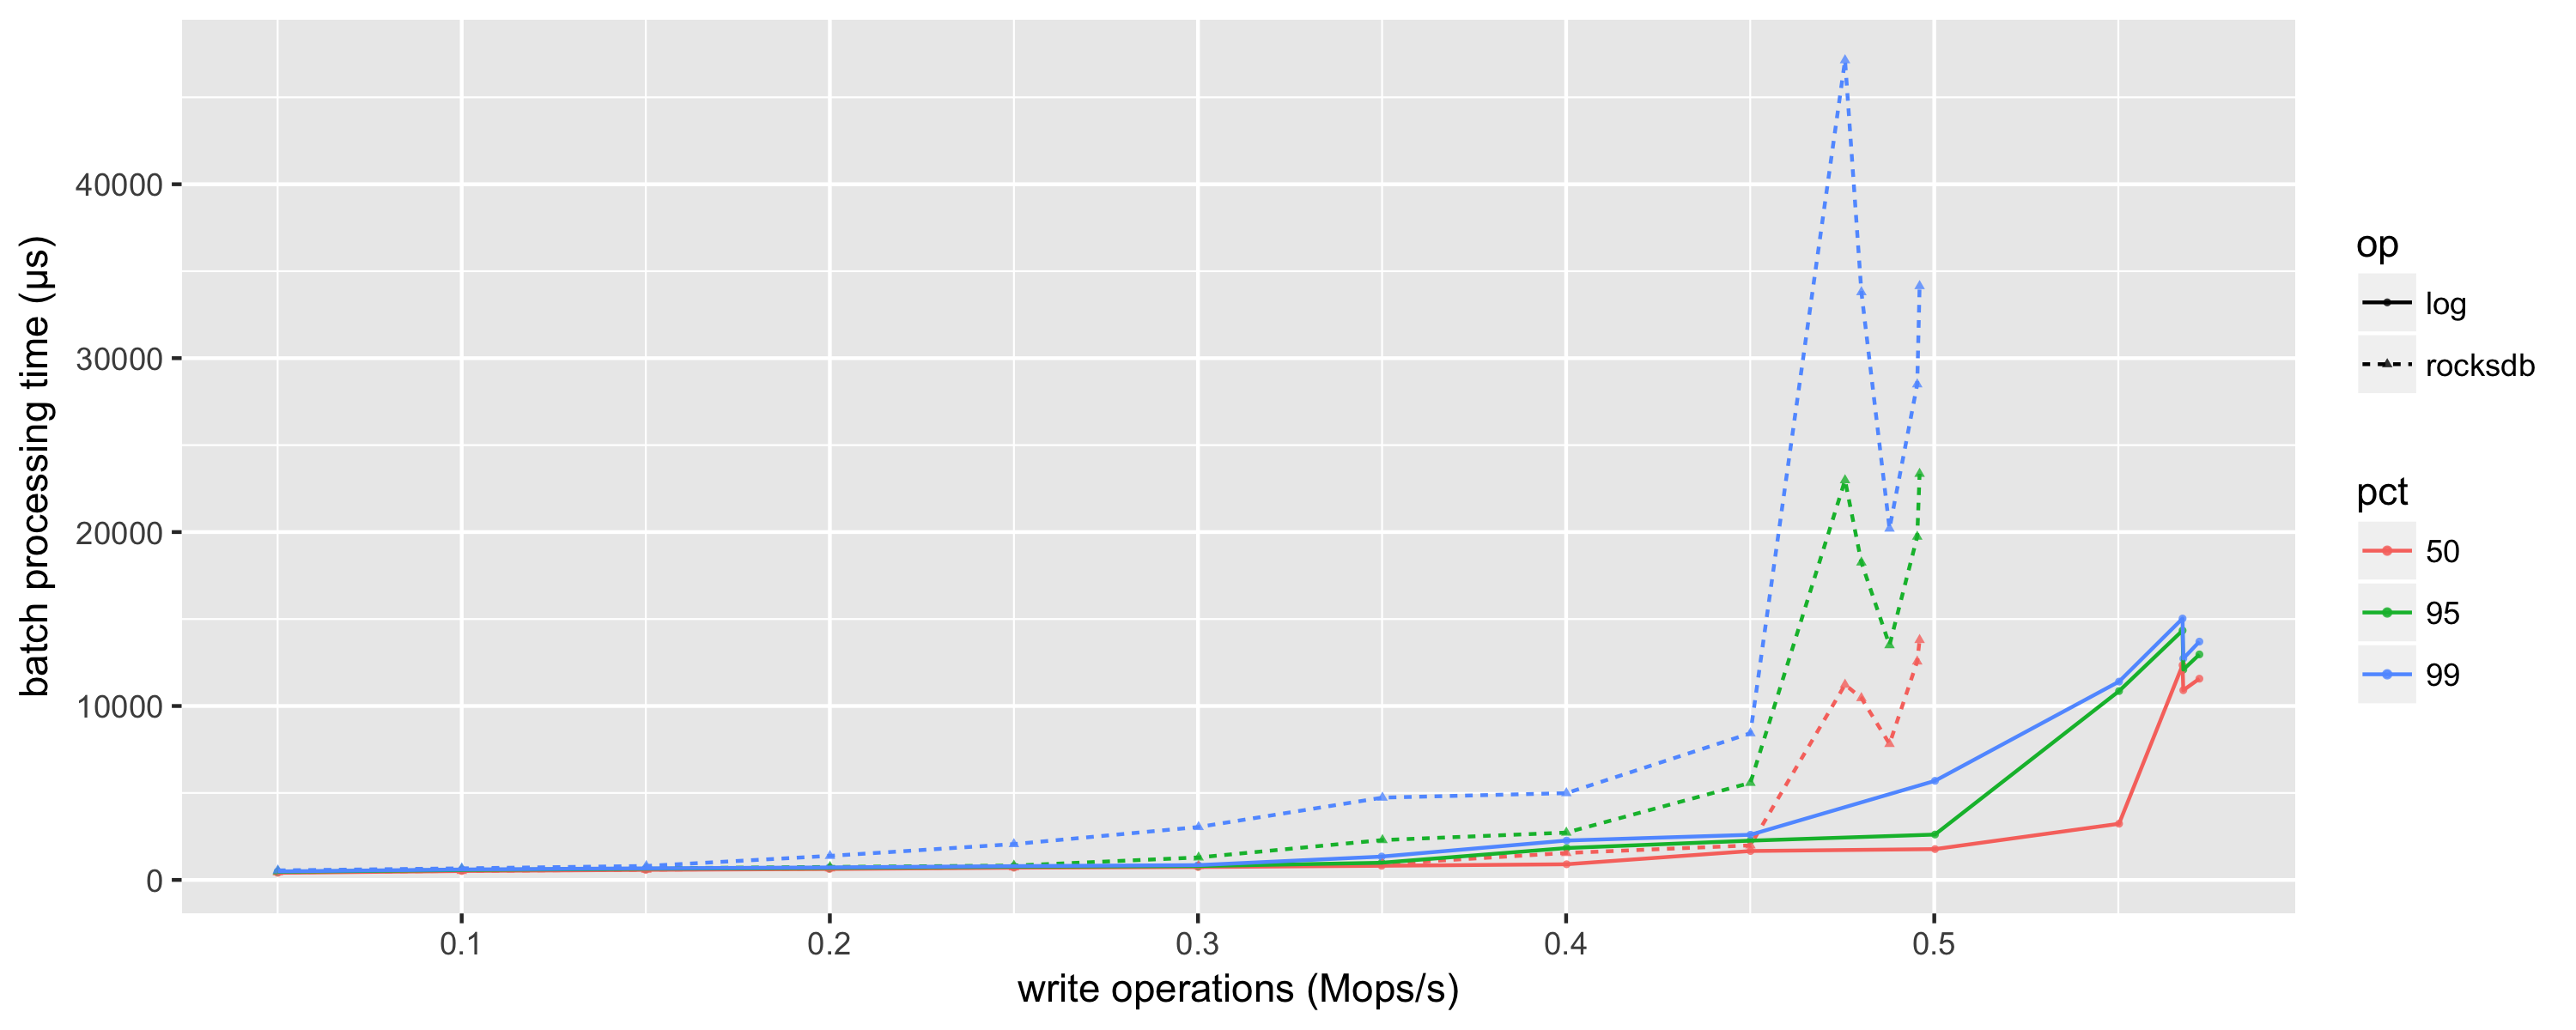
\includegraphics[width=\textwidth]{graphs/write-batch}
  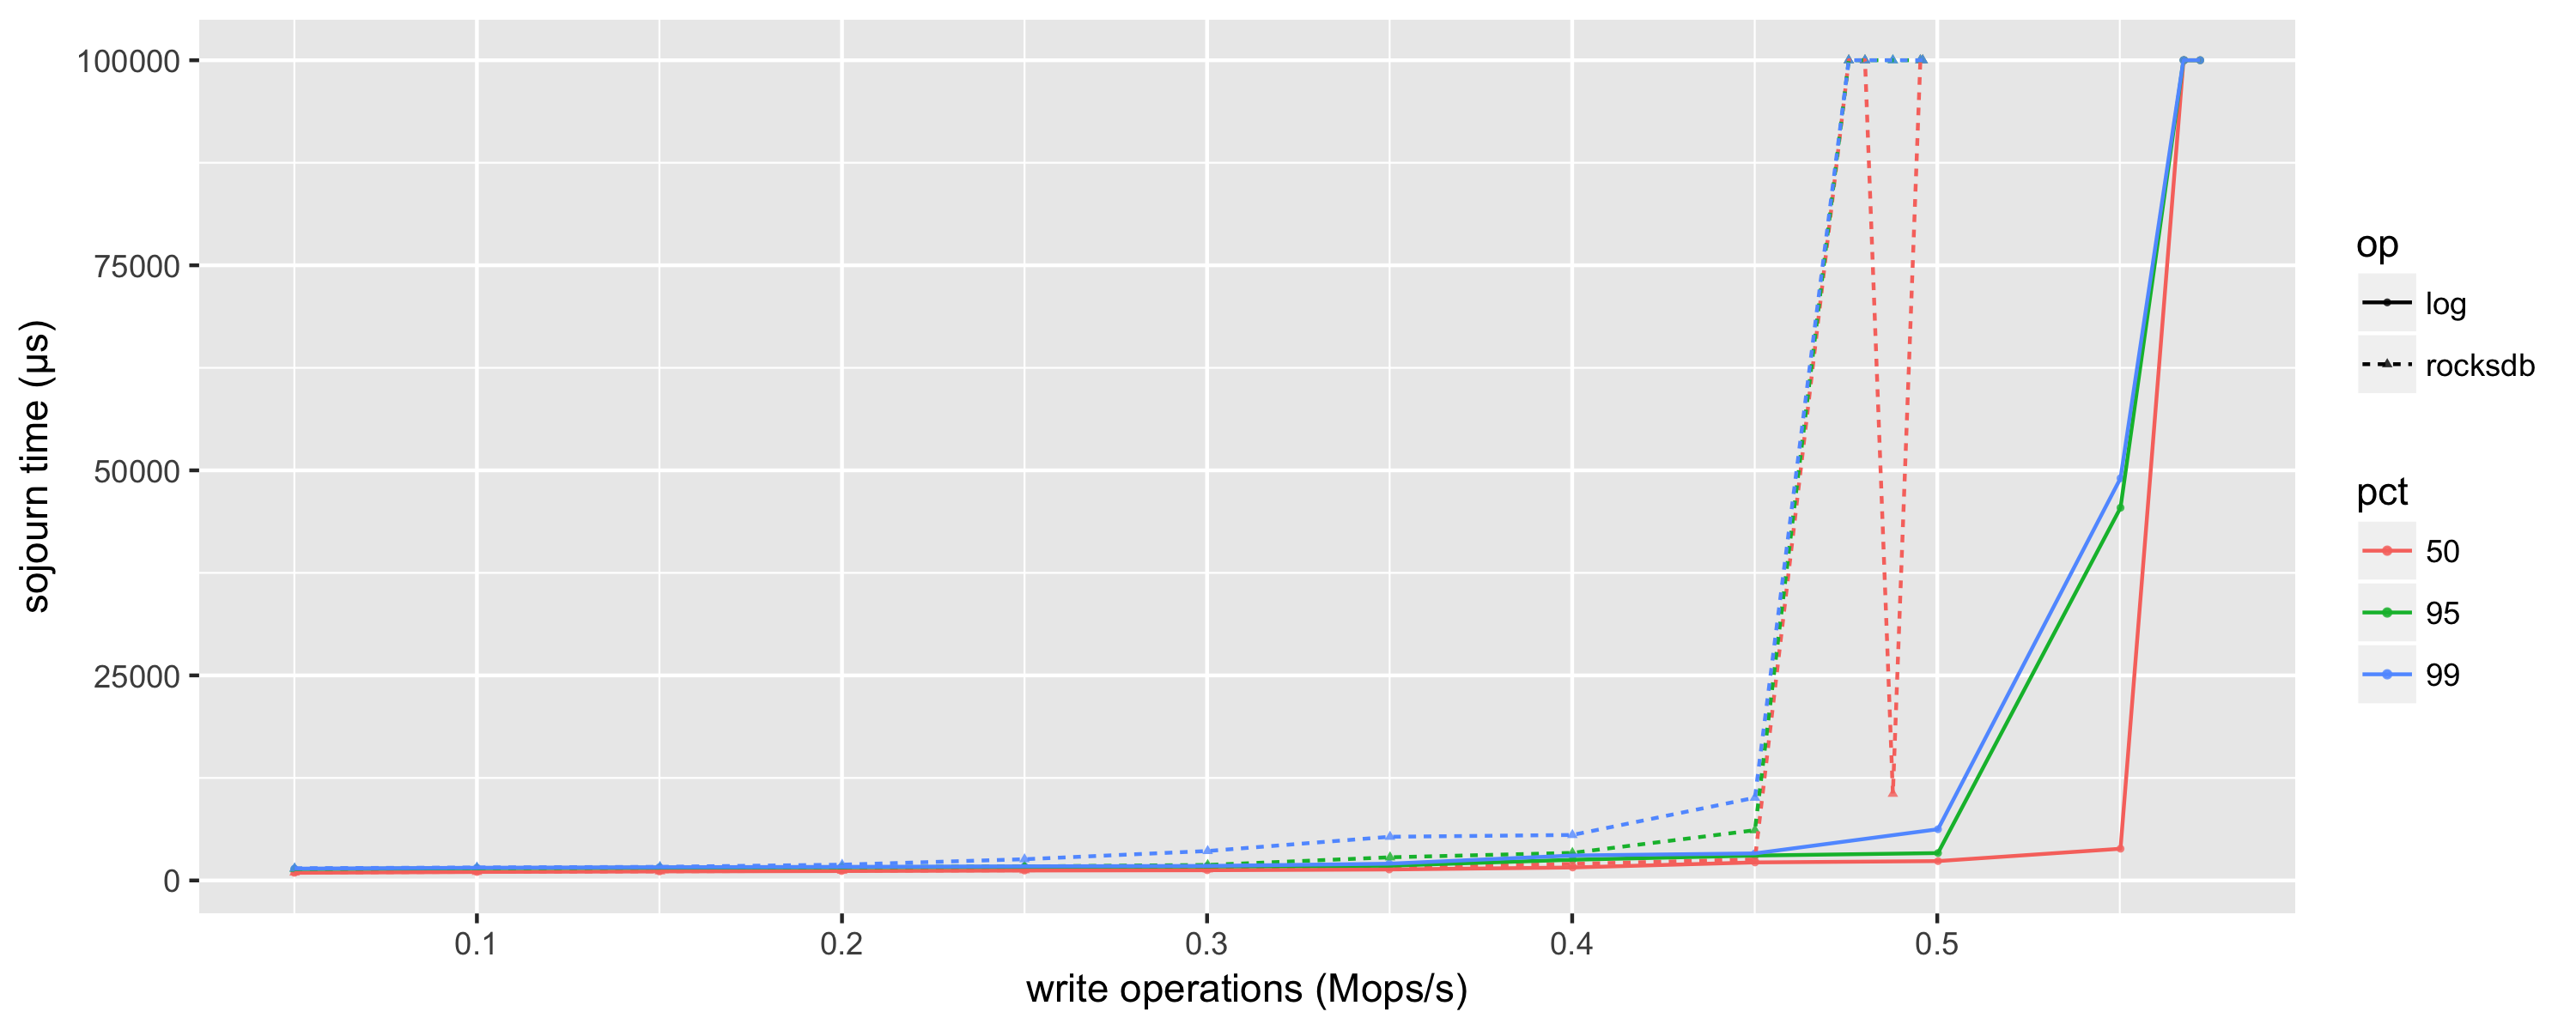
\includegraphics[width=\textwidth]{graphs/write-sjrn}
  \caption{\
    Write-only comparison of Soup's regular write-ahead log and RocksDB.\@ The
    topmost figure shows the latency from when the request was initiated, while
    the bottommost includes the time from the request was generated by the
    open-loop benchmark (see section~\ref{sec:vote-open-loop}).
  }\label{fig:graph-write}
\end{figure}

Materializing base node state to durable storage introduces a slight
write-latency penalty under load. This eventually translates to about a 10\%
decrease in maximum write-throughput, compared to the naive Soup log. Even
though the RocksDB write-ahead log is written to a different disk than its
SS-tables, the amount of data that has to be written to the RocksDB WAL with
\code{PersistentState} is still multiples more than with the Soup log. The
former has to include entries for every index a base node maintains, while the
latter only needs one entry for the update itself.

Additionally, writing to RocksDB's in-memory buffers is not a negligible cost,
especially considering serialization. Whereas the Soup log only needed to
serialize the update once, \code{PersistentState} needs to do so, in-part, once
for each index.

\todo{show a graph comparing memtable implementation speed?}

\section{Read-performance}

When measuring the overall read-performance of Soup as a system, a read heavy
\code{vote} benchmark is a good indicator. To analyze the impact of persisting
state to durable storage at the base nodes we want to ensure that we are
actually measuring the read performance of the \textit{base nodes} however, and
not the partial nodes further down the graph. Instead, we will make use of the
replay benchmark described in section~\ref{sec:bench-replay}, where each row is
read at most once, resulting in a full replay from the base nodes.

The database is pre-populated with 10 million rows, after which a small random
subset of the rows are read once. With \code{PersistentState}, Soup recovers
existing data between each test run, after flushing the disk caches.

\begin{figure}[H]
  \centering
  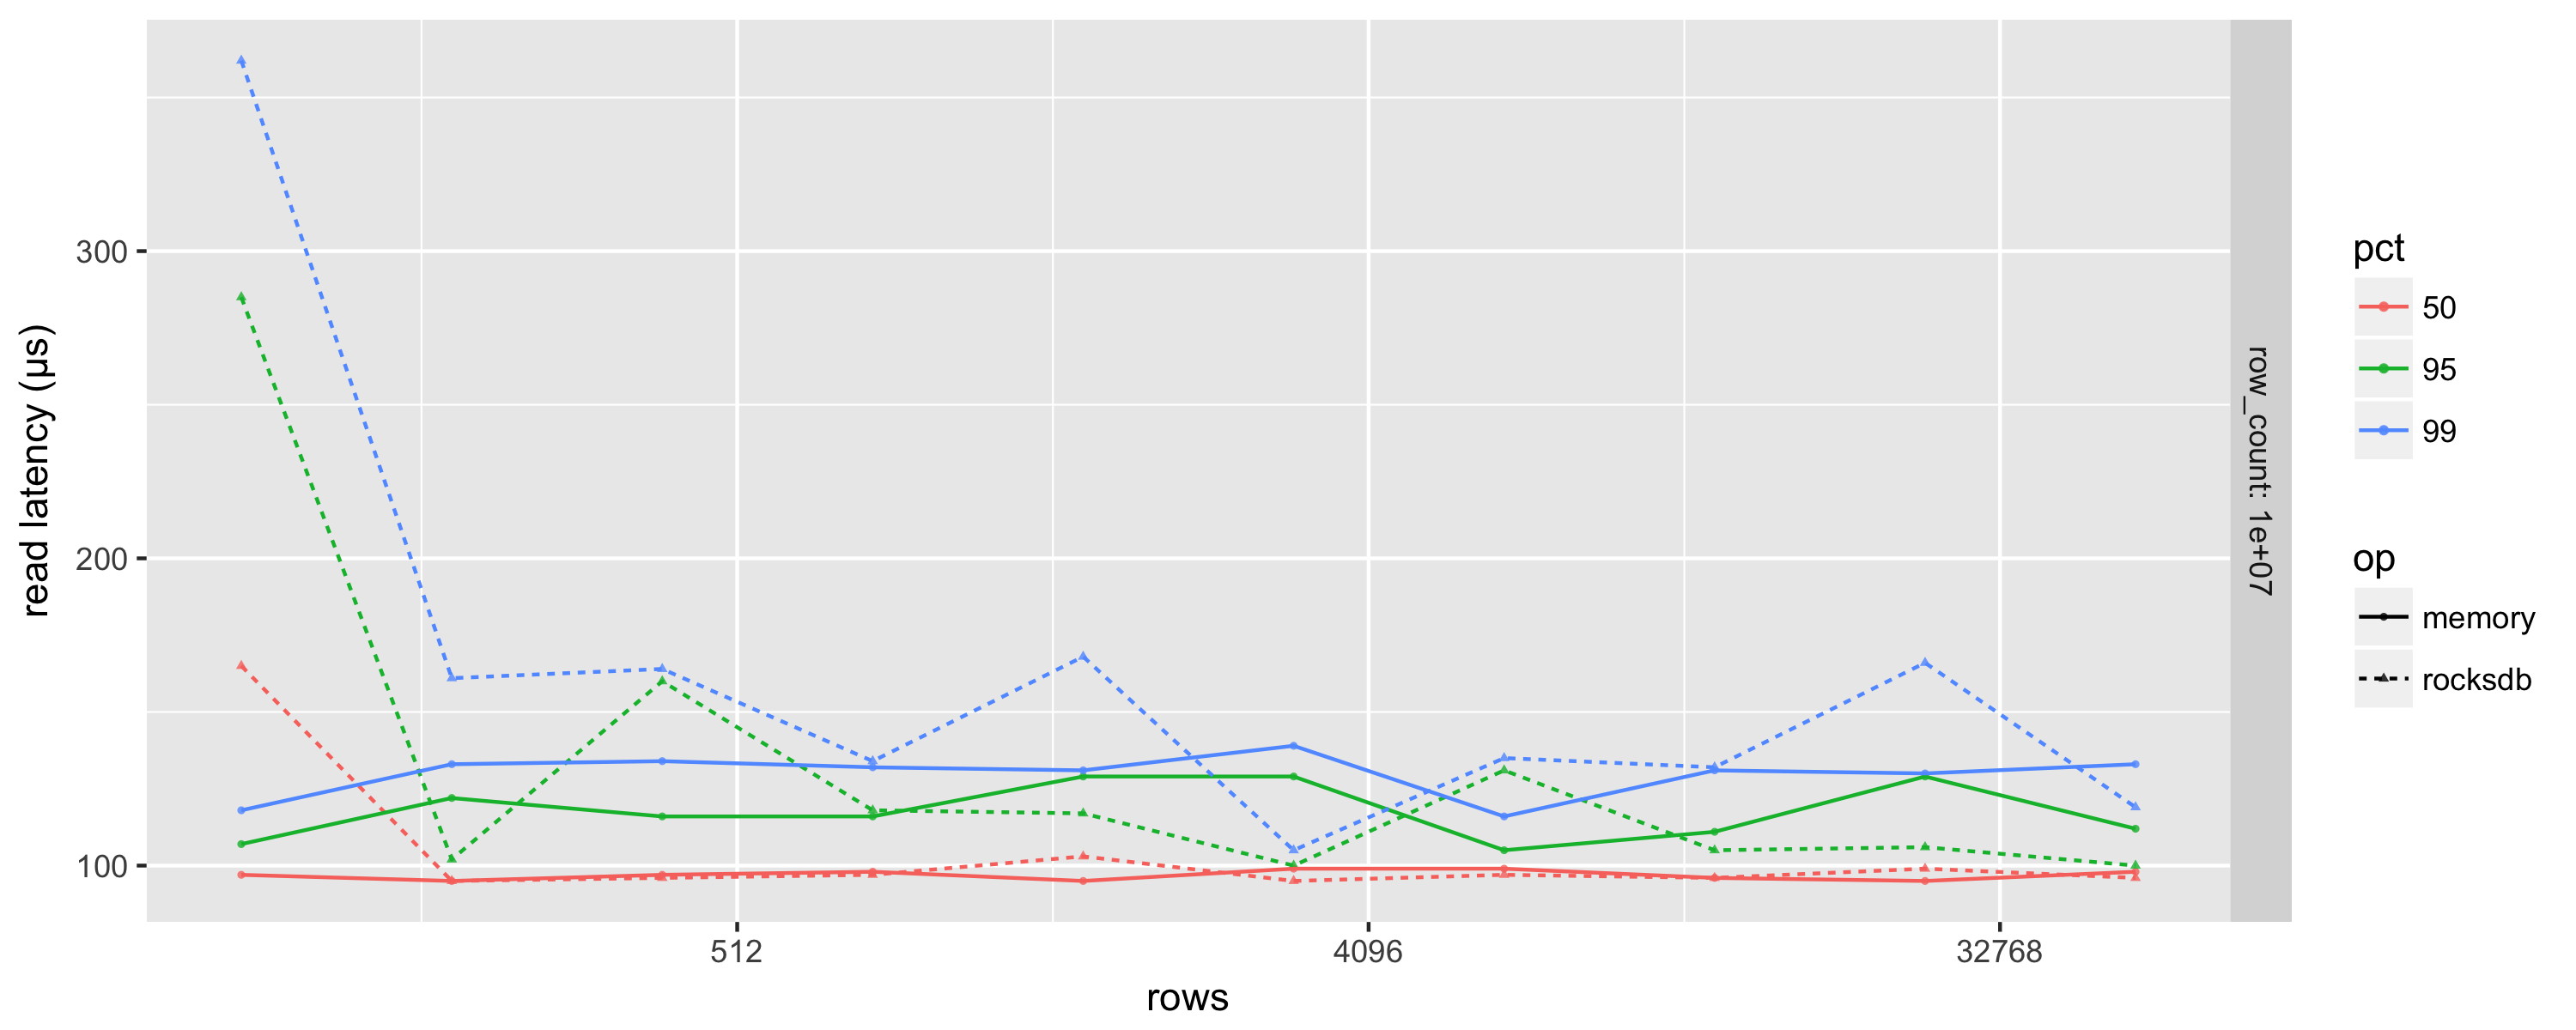
\includegraphics[width=\textwidth]{graphs/replay}
  \caption{\
    The replay performance of in-memory Soup compared to Soup with RocksDB.\@
  }\label{fig:graph-replay}
\end{figure}

\subsection{SS-table format}

RocksDB provides two separate SS-table implementations, \code{BlockBasedTable}
and \code{PlainTable}.

\todo{write more!}

\begin{figure}[H]
  \centering
  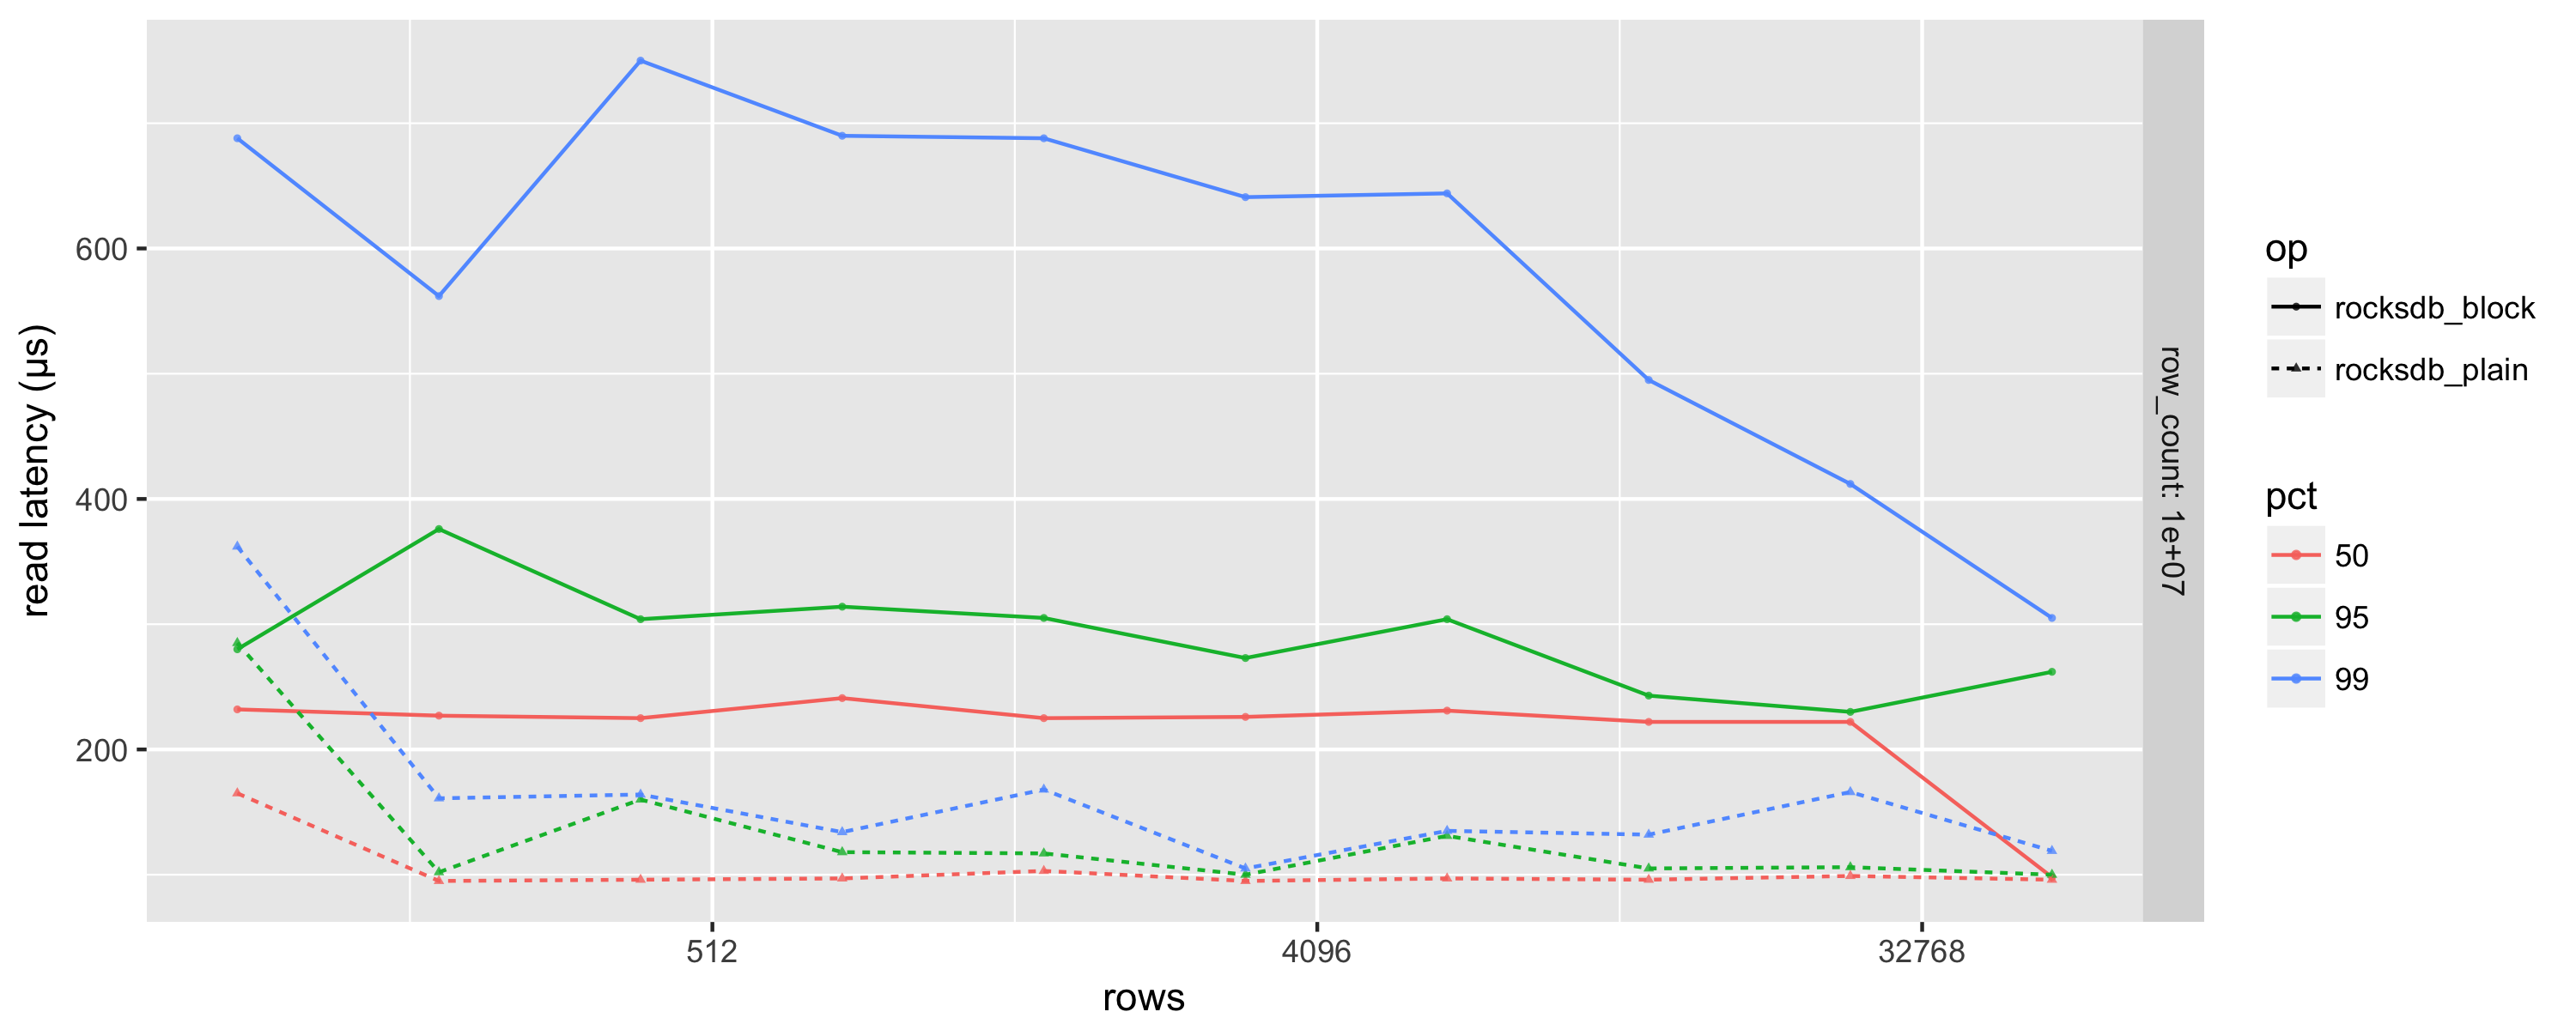
\includegraphics[width=\textwidth]{graphs/replay-table}
  \caption{\
    Soup replay performance comparison between \code{BlockBasedTable} and
    \code{PlainTable}.
  }\label{fig:graph-replay-table}
\end{figure}

\section{Mixed workload}

\section{Recovery}

The recovery benchmark introduced in section~\ref{sec:bench-recovery} helps us
compare the impact different durability strategies have on the time it takes to
recover after a failure. For every data point, the database is populated with
10K articles and a varying amount of votes divided evenly between the articles.
After population, Soup is restarted, while the time it takes to recover is
measured. The state is considered recovered when the total sum of votes returned from
reading all articles equal the actual amount of votes in the system---signified
as \textit{total} in figure~\ref{fig:graph-recovery}.

Unlike the other durability methods, recovering with durable base nodes does not
affect the partial nodes further down the graph---they remain empty until future
read operations trigger ancestor queries to the base nodes. Snapshotting, on the
other hand, brings all materialized nodes in the graph back to the state they
were in prior to crashing. This is the case for log-recovery as well, as updates
from the WAL propagate through the entire graph when recovering. To highlight
this divide, the time it takes to read a single key after recovering from a
durable base node application is measured as well, denoted as \textit{initial}
in figure~\ref{fig:graph-recovery}.

\begin{figure}[H]
  \centering
  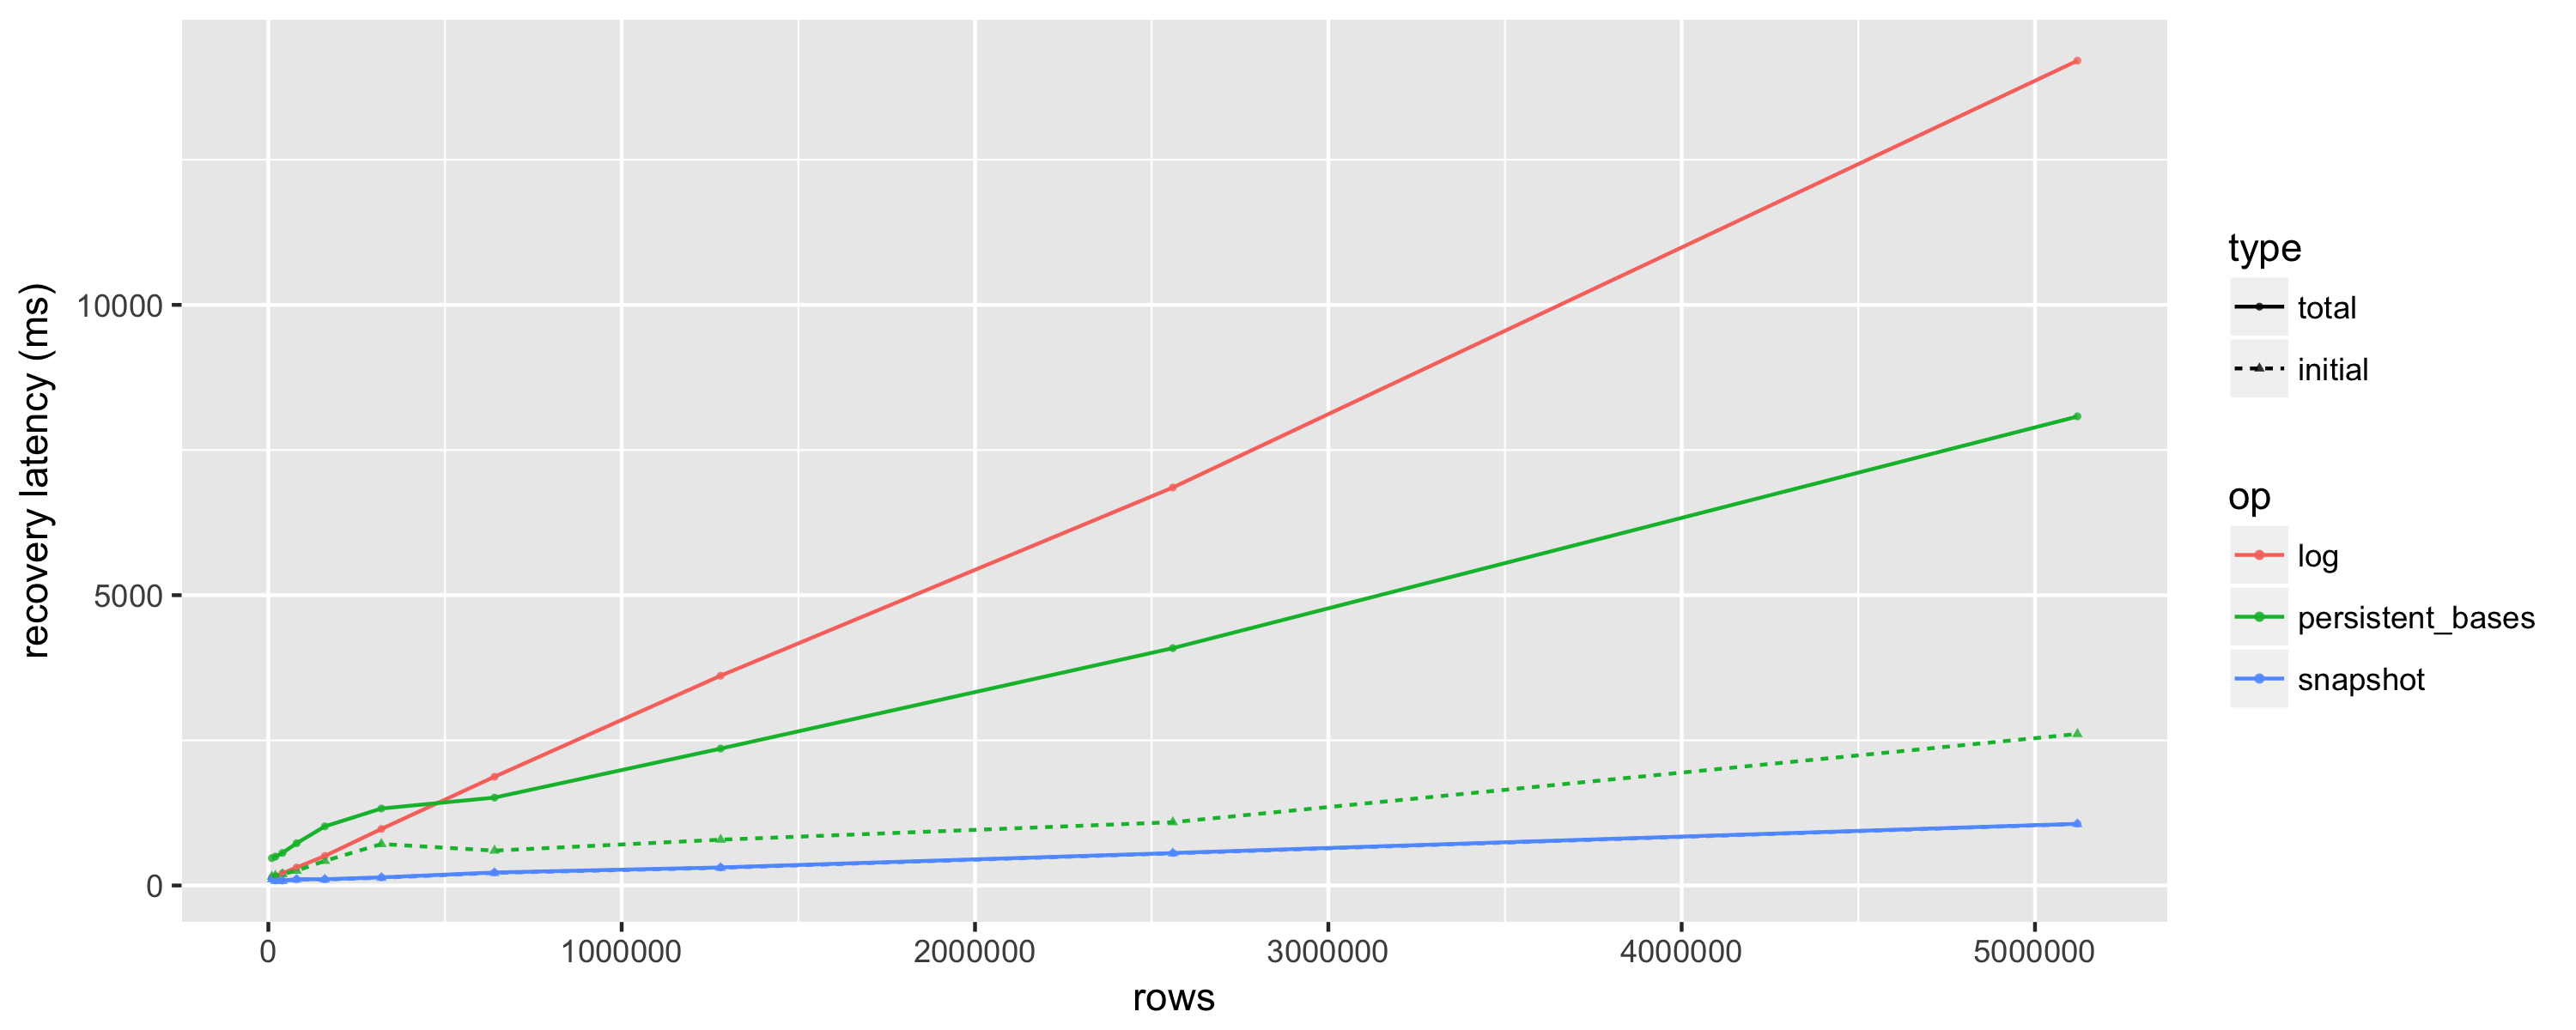
\includegraphics[width=\textwidth]{graphs/recovery}
  \caption{\
    The recovery benchmark measures the time it takes to recover after
    a failure. The \textit{initial} metric highlights the latency of reading a
    single key, while \textit{total} requires all reads to return the same
    result as prior to crashing.
  }\label{fig:graph-recovery}
\end{figure}

The results are pretty much as expected. Snapshotting returns all the
materialized nodes in the graph to their correct state, avoiding the need to
replay any state after recovering. The time it takes to recover still increases
after a while, with more data to read from disk. Log-based recovery needs to go
through \textit{all} updates since the beginning of time before it is considered
ready, resulting in poor performance. With durable base nodes, each read
requires a full replay from the bases---a significant latency penalty when the
row count goes up.

With \code{PersistentState}, the base nodes do not have to process any updates
at all when recovering. Restoring \code{PersistentState} to the correct state is
left to RocksDB, which puts a cap on recovery time by ensuring that its
write-ahead logs never grow beyond a given size. Recovering the actual database
files, the SS-tables, is ``free''---no data needs to be read into memory.

\subsection{Compressing Snapshots}

\todo{re-run benchmarks with compression}

\subsection{Write-performance with Snapshotting}

Snapshotting is a significant improvement to Soup's recovery situation, and a
step in the right direction for Soup as a production-ready system. Regardless,
it is only useful if Soup manages to maintain much of the same write-throughput
while performing regular snapshots.

To measure the performance penalty of snapshotting, we make use of the vote
benchmark described in section~\ref{sec:vote} and earlier in this chapter. The
benchmark compares the batch write latency at increasing throughput targets,
first without snapshotting and then with. The benchmark runs for 60 seconds,
performing a snapshot every 10 seconds.

\begin{figure}[H]
  \centering
  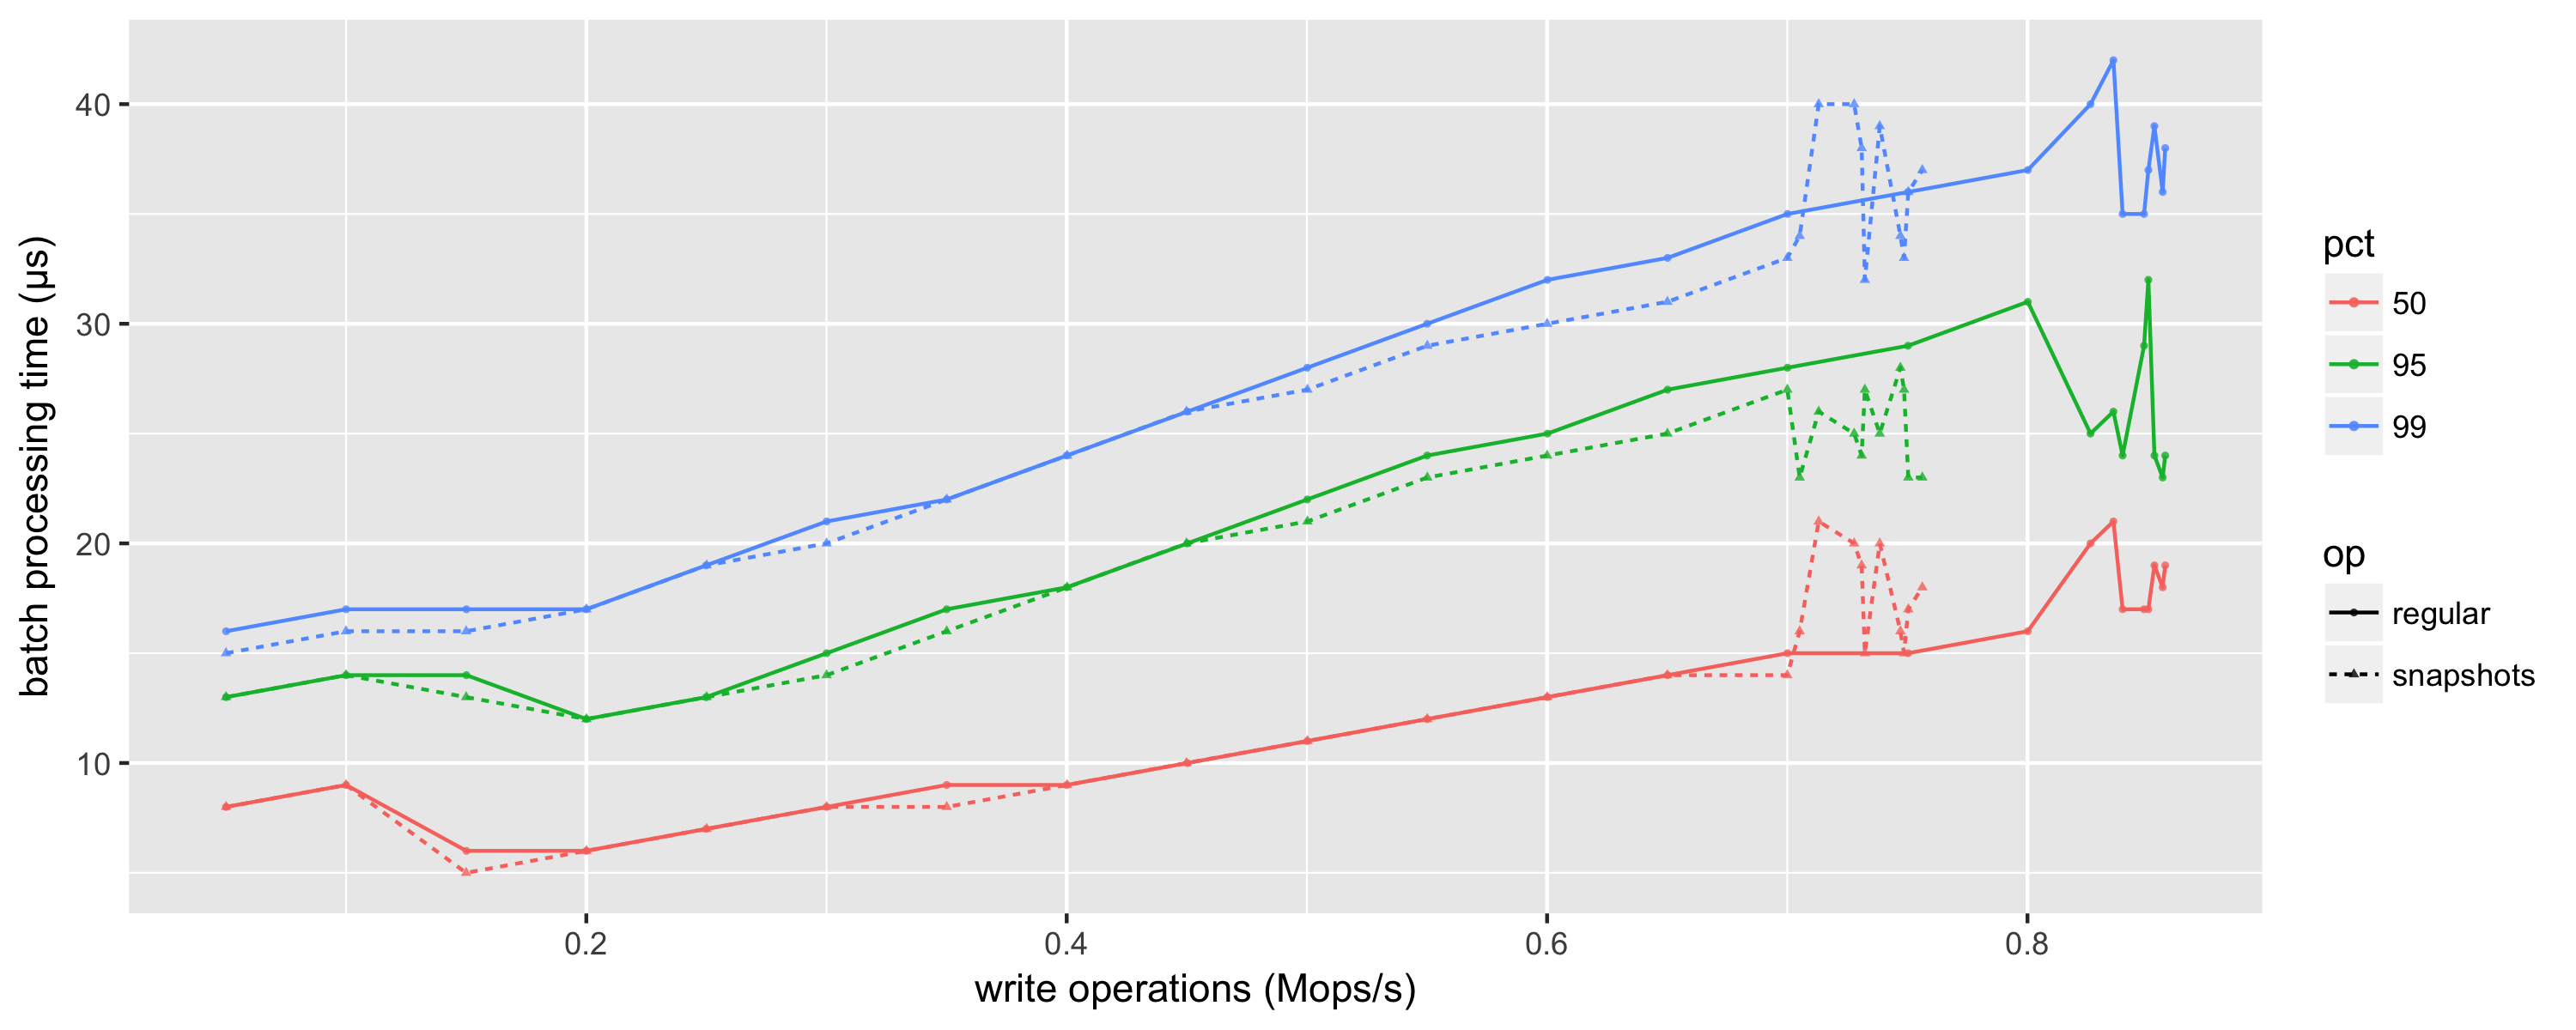
\includegraphics[width=\textwidth]{graphs/write-snapshot-batch}
  \caption{\
    Write-latency comparison with and without snapshotting (with a snapshot
    timeout of 10 seconds). Both use Soup's regular write-ahead log.
  }\label{fig:graph-snapshot}
\end{figure}

Most of the snapshotting work is performed in standalone snapshot workers,
running in threads separate from Soup's packet processing. Without this, the
throughput penalty would without doubt be much more significant than the 10\%
observed in figure~\ref{fig:graph-snapshot}. The penalty is a result of the full
state clone incurred at each materialized node during a snapshot.

\begin{figure}[H]
  \centering
  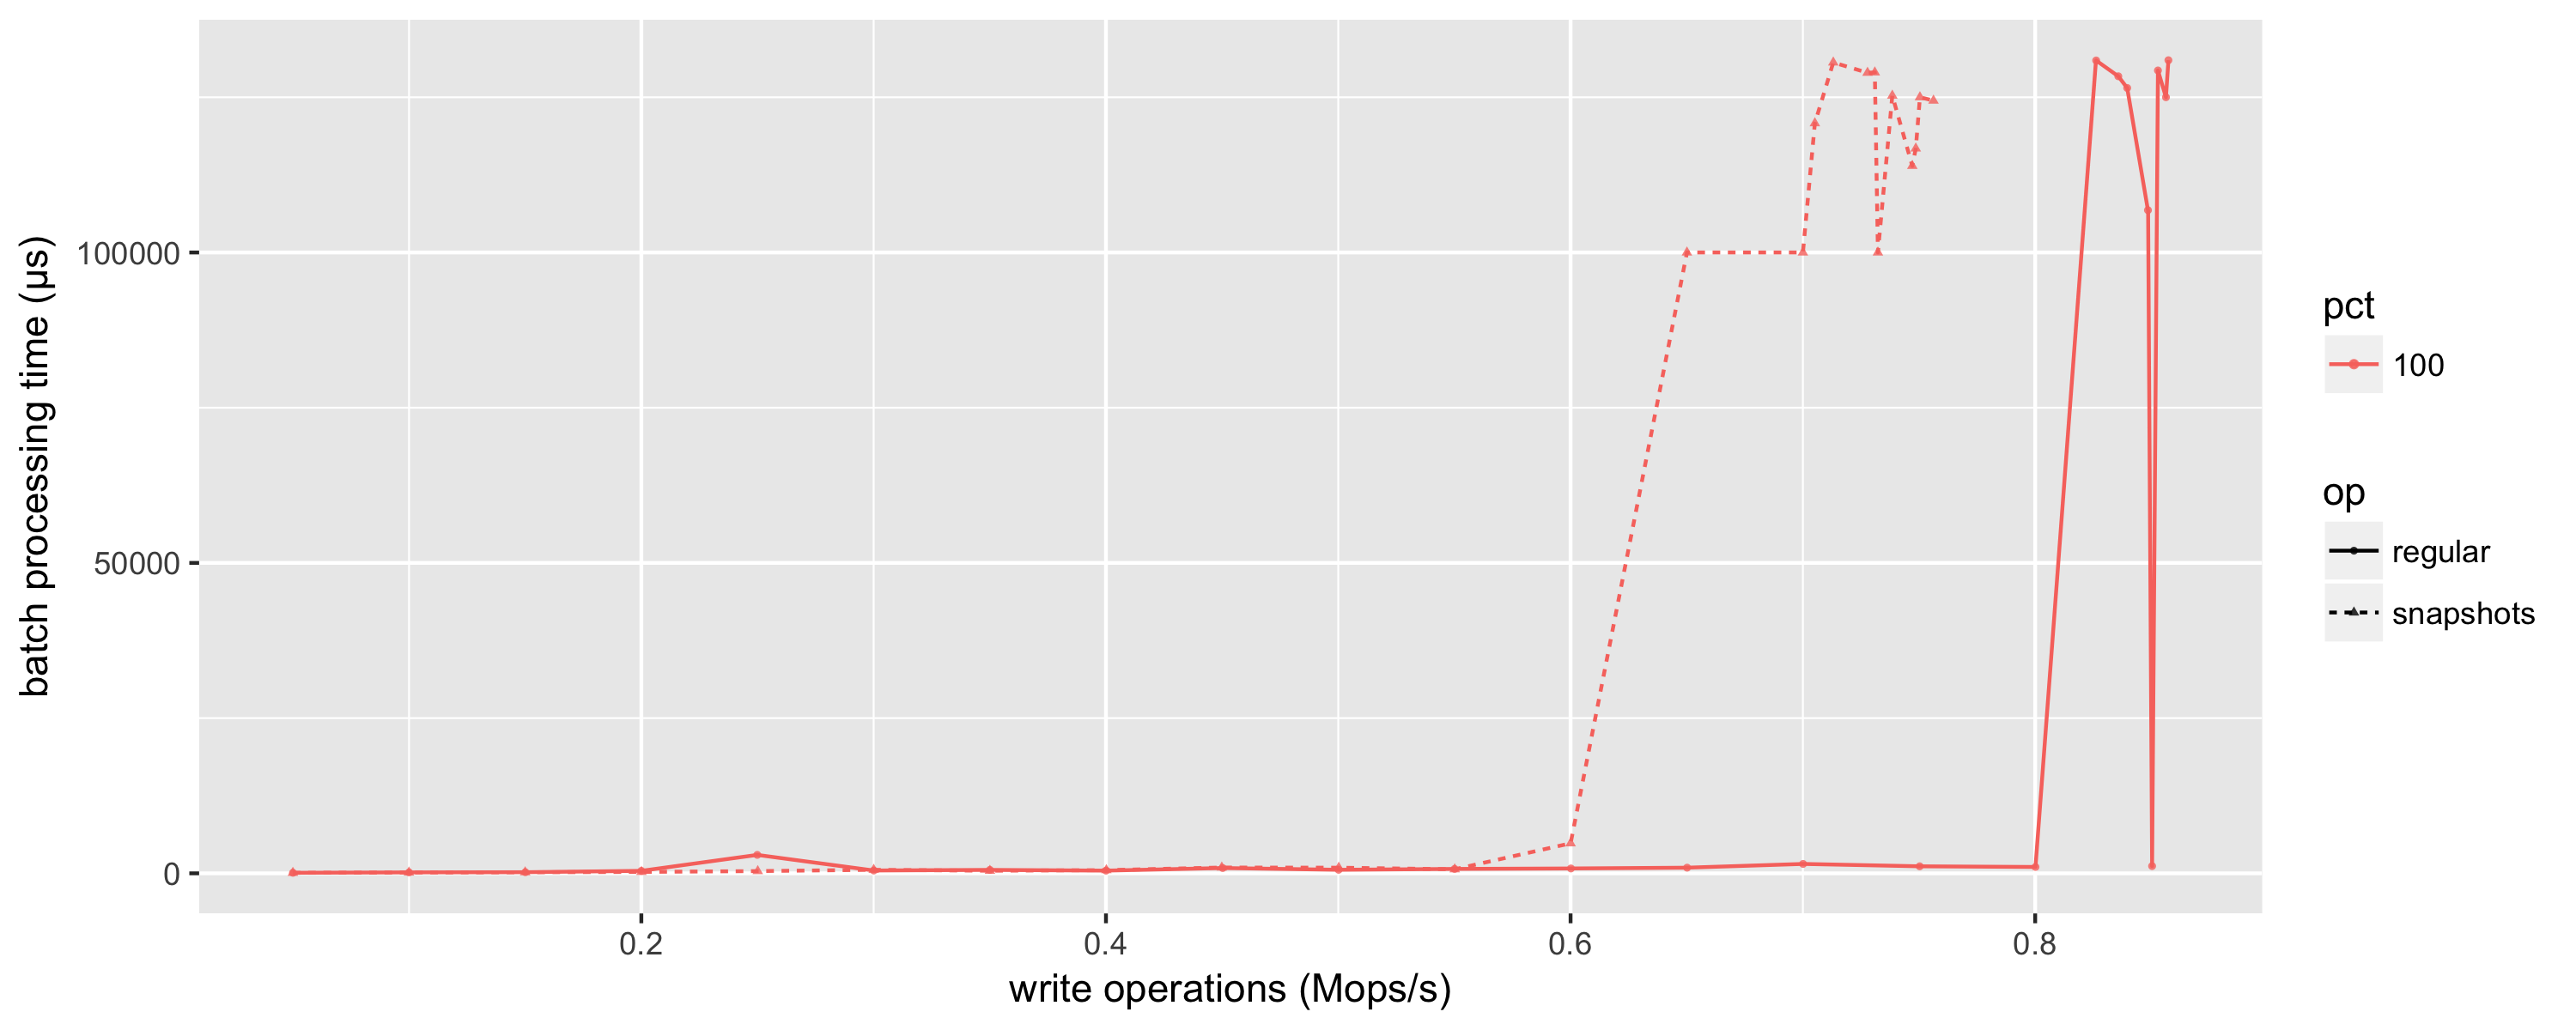
\includegraphics[width=\textwidth]{graphs/write-snapshot-100-batch}
  \caption{\
    100th percentile comparison, with and without snapshotting.
  }\label{fig:graph-snapshot-100}
\end{figure}

The first snapshot graph shows no increase in latency. With a snapshot timeout
of 10 seconds and a benchmark runtime of 60 seconds, snapshot occurrences are
probably too rare for it to show up in the 95th percentile. Looking at the 100th
percentile on the other hand, we can see the latency spiking at a lower
throughput than normal. At this point the state size is reasonably large,
resulting in non-trivial clone operations.

\chapter{Future Work}\label{chap:future-work}

\chapter{Conclusion}\label{chap:conclusion}

\section{Conclusion}


\section{Future Work}\label{sec:future-work}

\subsection{Snapshotting and Persistent Bases}

The \code{PersistentState} implementation described
in~\ref{chap:persistent-bases} removes the regular Soup write-ahead log in favor
of relying on RocksDB for durability. RocksDB maintains its own WAL,
which---unlike Soup's---is discarded when its updates are safely flushed to
durable storage. This is far better for recovery purposes, as it avoids the need
to go through a seemingly endless stream of updates to restore Soup back to a
pre-failure state. It does, on the other hand, complicate matters for
snapshotting.

Snapshotting relies on Soup's write-ahead log to recover updates that occur
after a snapshot is taken, prior to a failure. During recovery, the latest
snapshot is first restored, followed by log-based recovery for any remaining log
entries. Together they make sure that Soup recovers quickly, without degrading
its durability guarantees. With persistent bases the write-ahead log is
maintained internally by RocksDB, together with the decision of when to
eventually discard prior log files. Without the ability to replay log entries,
recovering using snapshotting would leave all other nodes than the base nodes in
an older state than before the crash.

Recovery using persistent bases leaves the partial nodes further down the graph
empty. This works fine because of Soup's replay system: any missing reads will
propagate all the way to the base nodes, resulting in the partial nodes
eventually reaching a similar state to the one they were in prior to crashing.
With snapshotting, the partial nodes would end up in an \textit{old} state,
instead of empty. This would prevent Soup from issuing base node replays,
effectively discarding the updates that happened after the last snapshot was
taken.

That leaves the question of how to replay any updates that happened after the
last snapshot was taken, while still relying on RocksDB's write-ahead log for
persistence. The first step would be to ensure that RocksDB never discards WAL
files until all its updates are included in a snapshot. Secondly, Soup's
recovery procedure would need to retrieve updates that happened after the last
snapshot was taken, directly from the RocksDB write-ahead logs. By including the
current snapshot identifier in all persisted updates, the recovery process would
be able to discern between updates that happened before and after the last
persisted snapshot.

\subsection{\code{PersistentState} serialization}

Both the keys and values persisted to RocksDB are serialized using
bincode (see section~\ref{sec:bincode}). While bincode performs well
compared to other serialization libraries,

\subsection{Uncoordinated snapshots}

Coordinating a global snapshot across the entire data-flow graph requires
unnecessary communication between the workers and the controller. Instead, the
question of finding the last valid snapshot could be left to the recovery
process, \eg by finding $ Min(epoch) $ across the nodes, or by following schemes
such as~\cite{falkirk}.

\subsection{Incremental snapshots}

The write-performance benchmark in section~\ref{sec:snapshot-write} showed a
10\% decrease in overall write throughput after introducing snapshotting. The
majority of the work is performed in separate snapshotting threads, leaving the
state clone operation as the culprit. To avoid cloning altogether, snapshots
would need to be maintained gradually, which could be achieved by maintaining a
buffer of changes between snapshots, which could then be forwarded to the
snapshotting worker and applied there. While this would avoid the need to clone
the entire state, snapshot workers would now need to keep an entirely duplicate
clone of the snapshot state in memory, effectively doubling Soup's memory usage.

Instead, snapshots could be maintained incrementally directly on durable
storage. This could make use of the same \code{PersistentState} implementation
used by persistent base nodes, either by having the snapshotting workers apply
received updates to RocksDB, or by doing so directly from each domain. This
would significantly reduce the write-amplification required to persist a
snapshot, by avoiding the need to write duplicate data to disk again and again.
By doing so, it would also minimize the risk of filling up the snapshot workers'
queues, which could now happen if the time it takes to serialize and persist a
single, possibly large, snapshot grows beyond the predefined snapshot interval.


\appendix
\chapter{Contributions}\label{chap:contributions}

The implementations described throughout this thesis have resulted in a series
of contributions to various open-source projects. This appendix lists a selected
subset of the \textit{pull requests} contributed to these projects, where a pull
request is simply a proposed unit of changes.

\newpage

\section{\code{distributary}}

\code{distributary} is the prototype implementation of Soup, written in Rust.

\begin{table}[H]
  \begin{tabular}{l l}
    \toprule
    \textbf{Title} & \textbf{Pull request}  \\ \midrule
    RocksDB Persistence & \url{https://git.io/vhf7w} (\#72) \\ \midrule
    SQLite Base Node Indices &
    \url{https://git.io/vhf7B} (\#58) \\ \midrule
    Initial Snapshotting Implementation & \url{https://git.io/vhf79} (\#54) \\ \midrule
    Recovery & \url{https://git.io/vhfbI} (\#37) \\ \midrule
    Arithmetic Expressions in Projections & \url{https://git.io/vhf7F} (\#35) \\ \midrule
    \code{AUTO\_INCREMENT} support & \url{https://git.io/vhf7b} (\#66) \\ \midrule
    Refactor \code{LookupResult} & \url{https://git.io/vhf5f} (\#76) \\ \midrule
    Remove generics from \code{State} & \url{https://git.io/vhf5k} (\#64) \\
    \midrule
    Materialization status in \code{graphviz} & \url{https://git.io/vhf5L}
    (\#51) \\ \midrule
    Use appropriate names for \\ literals and arithmetic expressions &
    \url{https://git.io/vhf5m} (\#45) \\ \midrule
    Add tests for \code{Extremum::MIN} & \url{https://git.io/vhf5G} (\#33) \\
    \bottomrule
  \end{tabular}

\end{table}

\section{\code{distributary-mysql}}

\code{distributary-mysql} is the MySQL protocol translation layer described in
section~\ref{sec:mysql-shim}.

\begin{table}[H]
  \begin{tabular}{l l}
    \toprule
    \textbf{Title} & \textbf{Pull request}  \\ \midrule
    \code{UPDATE} and \code{DELETE} support & \url{https://git.io/vhfdi} (\#12) \\
    \bottomrule
  \end{tabular}
\end{table}

\newpage

\section{\code{nom-sql}}

\code{nom-sql} is the SQL parser used by \code{distributary} and
\code{distributary-mysql}, written in Rust.

\begin{table}[H]
  \begin{tabular}{l l}
    \toprule
    \textbf{Title} & \textbf{Pull request}  \\ \midrule
    Add aliases to arithmetic expression & \url{https://git.io/vhf5D} (\#8) \\ \midrule
    Upgrade \code{nom} & \url{https://git.io/vhfdv} (\#13) \\ \midrule
    Move alias up to \code{FieldExpression} & \url{https://git.io/vhf5h} (\#15) \\ \midrule
    Attach the table name to keys \\ and columns in \code{CreateTableStatement} &
    \url{https://git.io/vhfdZ} (\#16) \\ \midrule
    Implement \code{fmt::Display} \\ for \code{ArithmeticExpression} & \url{https://git.io/vhf5F} (\#12) \\
    \bottomrule
  \end{tabular}
\end{table}

\section{\code{RocksDB}}

\code{RocksDB} is the key-value store described in section~\ref{sec:rocksdb},
which the durability layer in Soup is implemented on top of.

\begin{table}[H]
  \begin{tabular}{l l}
    \toprule
    \textbf{Title} & \textbf{Pull request}  \\ \midrule
    Add manual WAL flushing to the C API & \url{https://git.io/vhfb8} (\#3792) \\
    \bottomrule
  \end{tabular}
\end{table}

\newpage

\section{\code{rust-rocksdb}}

\code{rust-rocksdb} is a Rust wrapper library for \code{RocksDB}.

\begin{table}[H]
  \begin{tabular}{l l}
    \toprule
    \textbf{Title} & \textbf{Pull request}  \\ \midrule
    Add support for customizing \\ the memtable factory & \url{https://git.io/vhfAV} (\#180) \\ \midrule
    Support linking to other \\ compression libraries & \url{https://git.io/vhfAg} (\#185) \\ \midrule
    Add \code{set\_memtable\_prefix\_ratio} & \url{https://git.io/vhfAE} (\#181) \\ \midrule
    Make sure DB is dropped after all tests & \url{https://git.io/vhfAB} (\#183) \\ \midrule
    Add \code{index\_type} customization \\ to \code{BlockBasedOptions} & \url{https://git.io/vhfAl}
    (\#184) \\ \midrule
    Add \code{DBOptions.set\_wal\_dir} & \url{https://git.io/vhfN8} (\#186) \\
    \midrule
    Add \code{disable\_cache} method \\ to \code{BlockBasedOptions} & \url{https://git.io/vhfNC} (\#188) \\
    \bottomrule
  \end{tabular}
\end{table}


\printbibliography

\end{document}
